%%% LaTeX Template: Two column article
%%%
%%% Source: http://www.howtotex.com/
%%% Feel free to distribute this template, but please keep to referal to http://www.howtotex.com/ here.
%%% Date: February 2011

%%LINHA 37 \usepackage{indentfirst} % parágrafo / indentação
%%LINHA 38 \usepackage{setspace} espaço entre linhas

%%% Preamble
\documentclass[	DIV=calc,%
							paper=a4,%
							fontsize=12pt,%
							onecolumn]{scrartcl}	 					% KOMA-article class

\usepackage{lipsum}													% Package to create dummy text
\usepackage[brazil]{babel}										% English language/hyphenation
\usepackage[protrusion=true,expansion=true]{microtype}				% Better typography
\usepackage{amsmath,amsfonts,amsthm}					% Math packages
\usepackage[pdftex]{graphicx}									% Enable pdflatex
\usepackage[svgnames]{xcolor}									% Enabling colors by their 'svgnames'
\usepackage[hang, small,labelfont=bf,up,textfont=it,up]{caption}	% Custom captions under/above floats
\usepackage{epstopdf}												% Converts .eps to .pdf
\usepackage{subfig}													% Subfigures
\usepackage{booktabs}												% Nicer tables
\usepackage{fix-cm}													% Custom fontsizes
\usepackage[utf8]{inputenc}
\usepackage[top=3cm, bottom=2cm, left=3cm, right=2cm]{geometry}
\usepackage[ddmmyyyy]{datetime}
\usepackage{pdfpages}
\usepackage{hyperref}
\hypersetup{
	colorlinks,
	citecolor=blue,
	filecolor=blue,
	linkcolor=black,
	urlcolor=black
}
\addto\captionsenglish{%
	\renewcommand\tablename{Tabela}
	\renewcommand\figurename{Figura}
} 
 
%%% Custom sectioning (sectsty package)
\usepackage{sectsty}													% Custom sectioning (see below)
\usepackage{indentfirst} % parágrafo / indentação
\usepackage{setspace}

\allsectionsfont{%															% Change font of al section commands
	\usefont{OT1}{phv}{b}{n}%										% bch-b-n: CharterBT-Bold font
	}

\sectionfont{%																% Change font of \section command
	\usefont{OT1}{phv}{b}{n}%										% bch-b-n: CharterBT-Bold font
	}

%%% Headers and footers
\usepackage{fancyhdr}												% Needed to define custom headers/footers
	\pagestyle{fancy}														% Enabling the custom headers/footers
\usepackage{lastpage}	

% Header (empty)
\lhead{}
\chead{}
\rhead{}
% Footer (you may change this to your own needs)

%% ====================================
%% ====================================
%% mude o rodape  do projeto
%% ====================================
%% ====================================

\lfoot{\footnotesize \texttt{Cabeamento estruturado} \textbullet ~Instituto Ambiental do Paraná}
\cfoot{}
\rfoot{\footnotesize página \thepage\ de \pageref{LastPage}}	% "Page 1 of 2"
\renewcommand{\headrulewidth}{0.0pt}
\renewcommand{\footrulewidth}{0.4pt}

%%% Creating an initial of the very first character of the content
\usepackage{lettrine}
\newcommand{\initial}[1]{%
     \lettrine[lines=3,lhang=0.3,nindent=0em]{
     				\color{DarkGoldenrod}
     				{\textsf{#1}}}{}}

%%% Title, author and date metadata
\usepackage{titling}															% For custom titles

\newcommand{\HorRule}{\color{DarkGoldenrod}%			% Creating a horizontal rule
									  	\rule{\linewidth}{1pt}%
										}

\pretitle{\vspace{-30pt} \begin{flushleft} \HorRule 
				\fontsize{40}{40} \usefont{OT1}{phv}{b}{n} \color{DarkRed} \selectfont 
				}

%% ====================================
%% ====================================
%% mude o titulo  do projeto
%% ====================================
%% ====================================

\title{Projeto de cabeamento estruturado na Infraestrutura de Rede do Instituto Ambiental do Paraná}					% Title of your article goes here

%% ====================================
\posttitle{\par\end{flushleft}\vskip 0.5em}
\preauthor{\begin{flushleft}
					\large \lineskip 0.5em \usefont{OT1}{phv}{b}{sl} \color{DarkRed}}
\author{André Luis Finatto
	\\ Diogo Witt,
	\\ Jedielson de Souza,
	\\ Paulo Cesar Cardoso de Campos \vspace{1cm}}  	% Author name goes here


\postauthor{\footnotesize \usefont{OT1}{phv}{m}{sl} \color{Black} 
					\\Universidade Tecnológica Federal do Paraná - Câmpus Cornélio Procópio 								% Institution of author
					\par\end{flushleft}\HorRule}

\date{}																				% No date

%%% Begin document
\begin{document}
\maketitle
\thispagestyle{fancy} 	
\thispagestyle{empty}		% Enabling the custom headers/footers for the first page 
% The first character should be within \initial{}
%% ====================================
%% ====================================
%% mude o resumo  do projeto
%% ====================================
%% ====================================
\initial{O}\textbf{presente projeto visa apresentar uma reestruturação fictícia na infraestrutura baseada no ambiente real do Instituto Ambiental do Paraná. O Projeto aborda o levantamento da planta física, elaboração da planta lógica e equipamentos passivos da rede.}
%% ====================================

\begin{figure}
	\centering
	
\includegraphics{utfpr}
\end{figure}

\vspace{1,5cm}
\centerline{\textit{\textbf{\today}}}

\clearpage
\renewcommand*\listfigurename{Lista de figuras}
\listoffigures
\renewcommand*\listtablename{Lista de tabelas}
\listoftables

\clearpage
\renewcommand{\contentsname}{Sumário}
\tableofcontents
\clearpage
%% ====================================
%% ====================================
%% Inicio do texto
%% ====================================
%% ====================================
\section{Introdução}
\onehalfspacing % espaçamento 1,5 entre linhas
Este projeto tem como propósito levantar os requisitos e propor soluções no âmbito da rede de computadores do Instituto Ambiental do Paraná - Escritório Regional de Curitiba – IAP ERCBA, constituindo-se no órgão de pesquisa que dá embasamento tecnológico as políticas públicas de desenvolvimento rural do Estado do Paraná.\par
O ambiente do Instituto Ambiental do Paraná é formado por técnicos responsáveis por trabalhos e rotinas administrativas, além de emissão de licenças e análises ambientais.\par
Atualmente são utilizados 33 \textit{desktops}, além de 27 ramais telefônicos, duas impressoras e uma central telefônica.
O objetivo do presente projeto é definir requisitos, materiais e planos de execução para conectar os vários elementos computacionais, com intuito de se utilizar de maneira compartilhada e eficiente todos seus recursos disponíveis. \par
Assim sendo, o presente projeto constitui-se no primeiro item de documentação da rede a ser implantada.

\subsection{Benefícios}
Após a execução do projeto, a infraestrutura de redes e dados estará mais segura, proverá maior desempenho e estará menos suscetível a intercorrências que possam vir a causar sua paralisação. O suporte será mais simples e rápido, além de facilitar em possíveis mudanças de posições de equipamentos.

\subsection{Organizações Envolvidas}
%Coloque o nome de todas as organizações envolvidas. Se for um projeto real, identifique quais as responsabilidades de cada uma das organizações. É comum que em um projeto de redes (cabeamento), temos várias organizações, sendo que cada uma delas com uma determinada responsabilidade.
%Sugestão: crie uma tabela contento a relação delas.
\begin{table}[h!] % coloque h! para forcar a posicao
\onehalfspacing
\centering
\caption{Atividades e respectivos responsáveis}
\vspace{0.5cm}
\label{tab1}
\resizebox{\textwidth}{!}{%
	\begin{tabular}{|c|c|}
		\hline
		\textbf{Responsabilidade}                                           & \textbf{Organização}            \\ \hline
		Serviços de Internet 1                                              & Empresa Provedora de Internet 1 \\ \hline
		Serviços de Internet 2 – (Redundância)                              & Empresa Provedora de Internet 1 \\ \hline
		Levantamento de Requisitos                                          & Grupo                           \\ \hline
		Desenvolvimento do Projeto                                          & Grupo                           \\ \hline
		Orçamento dos ativos e passivos de rede                             & Grupo                           \\ \hline
		Aquisição dos ativos e passivos de rede                             & Setor Compras - Contratante     \\ \hline
		Instalação de eletrocalhas                                          & Contratante                     \\ \hline
		Instalações elétricas adequadas (tomadas, aterramento, para-raios)  & Contratante                     \\ \hline
		Instalação dos pontos de rede Ethernet (descritos na planta lógica) & Grupo                           \\ \hline
		Passagem do cabeamento (horizontal e backbone)                      & Grupo                           \\ \hline
		Instalação e configuração de todos ativos e passivos de rede        & Grupo                           \\ \hline
	\end{tabular}%
}

\end{table}

\section{Estado atual}
%Aprente o estado atual da rede. Caso não tenha rede, desconsiderar esta seção.
%Caso tenha rede, deixe claro:
%\begin{itemize}
%	\item  os passivos de rede atuais:path panels, cabos, etc..;
%	\item as principais reclamações dos usuários. Qual o principal motivo da reestruturação? Efetue uma pesquisa junto aos colaboradores para determinar quais problemas a rede apresenta.
%	\item Observações. Analise a rede e verifique se há estruturas que não se enquadram nas normas ou que indicam suspeita de problemas.
%\end{itemize}
Atualmente tanto a estrutura predial quanto o cabeamento do ambiente estão bastante deteriorados.\par
É possível identificar vazamentos e infiltrações no prédio que podem afetar a rede de dados e dispositivos, uma vez que o cabeamento não está devidamente acomodado dentro de canaletas e conduítes apropriados. Há ainda cabos expostos nas salas, que podem provocar acidentes, serem arrancados e arrebentados ou induzir pessoas a realizarem conexões indevidas.\par
Além do já mencionado, o cabeamento não é certificado. Não são usados \textit{patch cords} em todas as estações, existindo cabos fabricados a mão que podem não entregar o desempenho desejado e sofrer com interferências.\par
Nem todos os cabos estão identificados e a acomodação dos \textit{patch cords} dentro dos racks não foi realizada da maneira adequada, o que dificulta a resolução de falhas e a identificação dos elementos na rede.
\begin{figure}[h!]
	\centering
	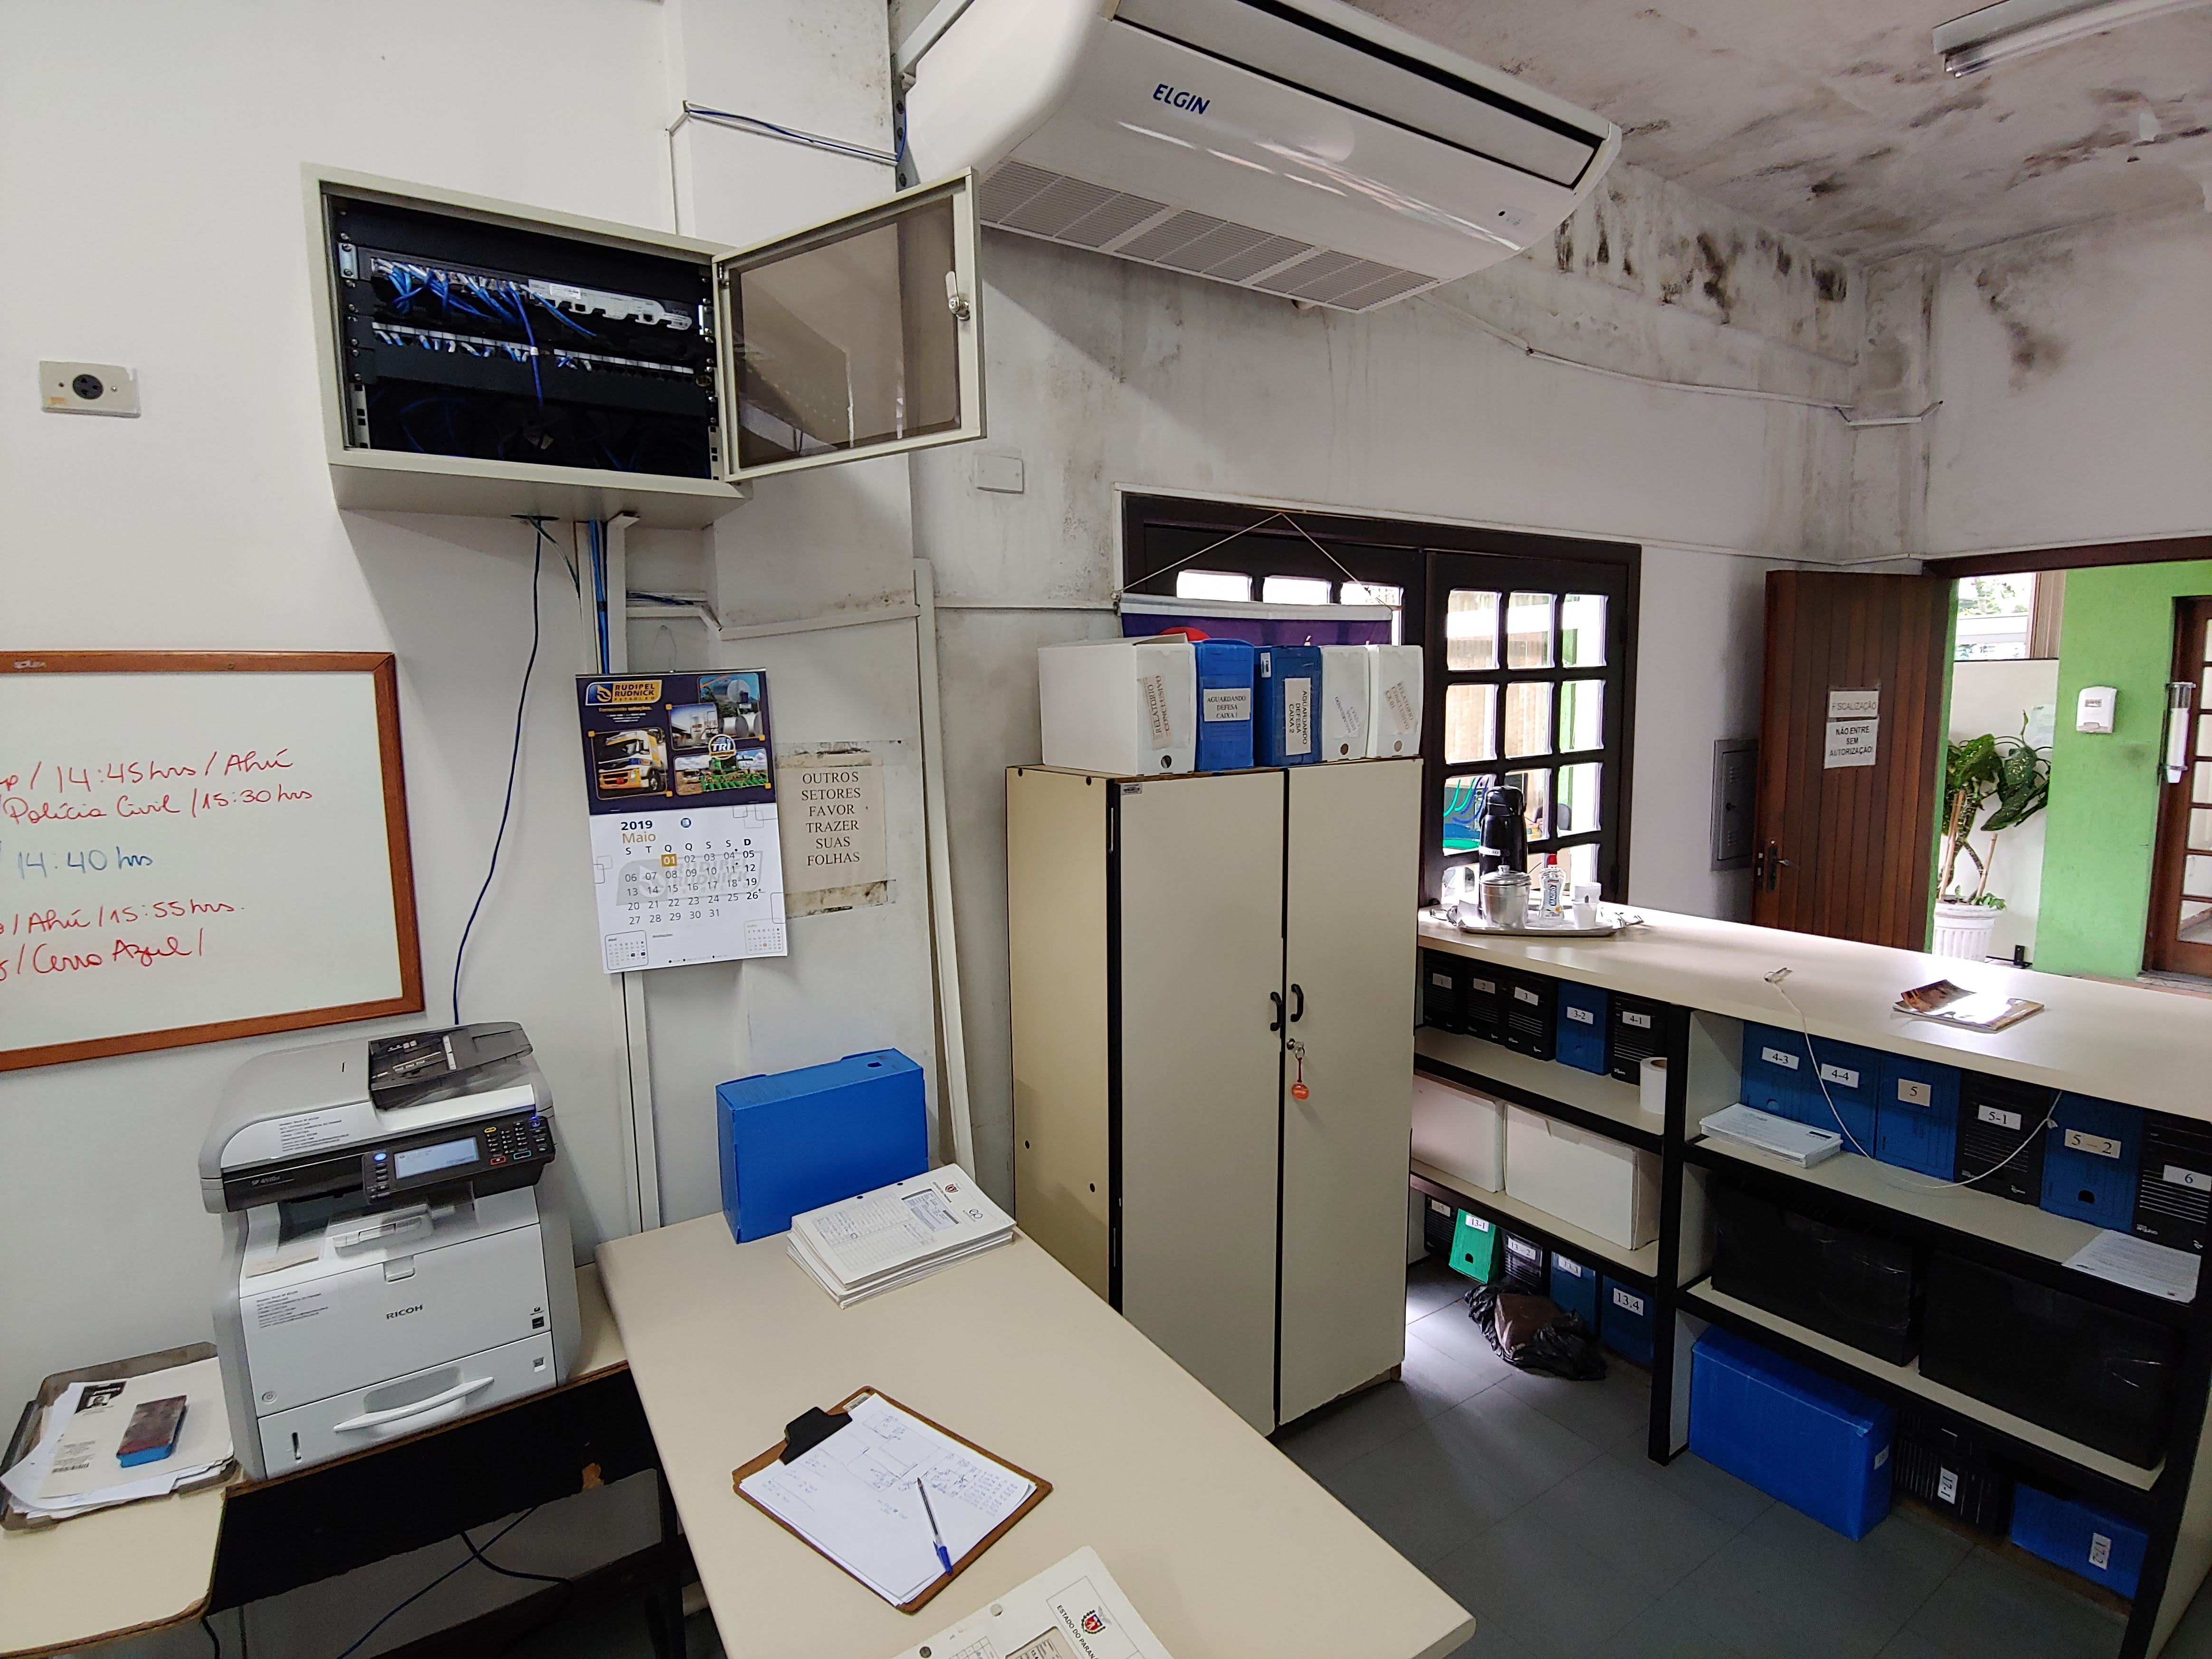
\includegraphics[width=0.8\textwidth]{figura10.jpg}
	\caption[Setor de Fiscalização]{Setor de Fiscalização}
	\label{figura10}
\end{figure}

\begin{figure}[h!]
	\centering
	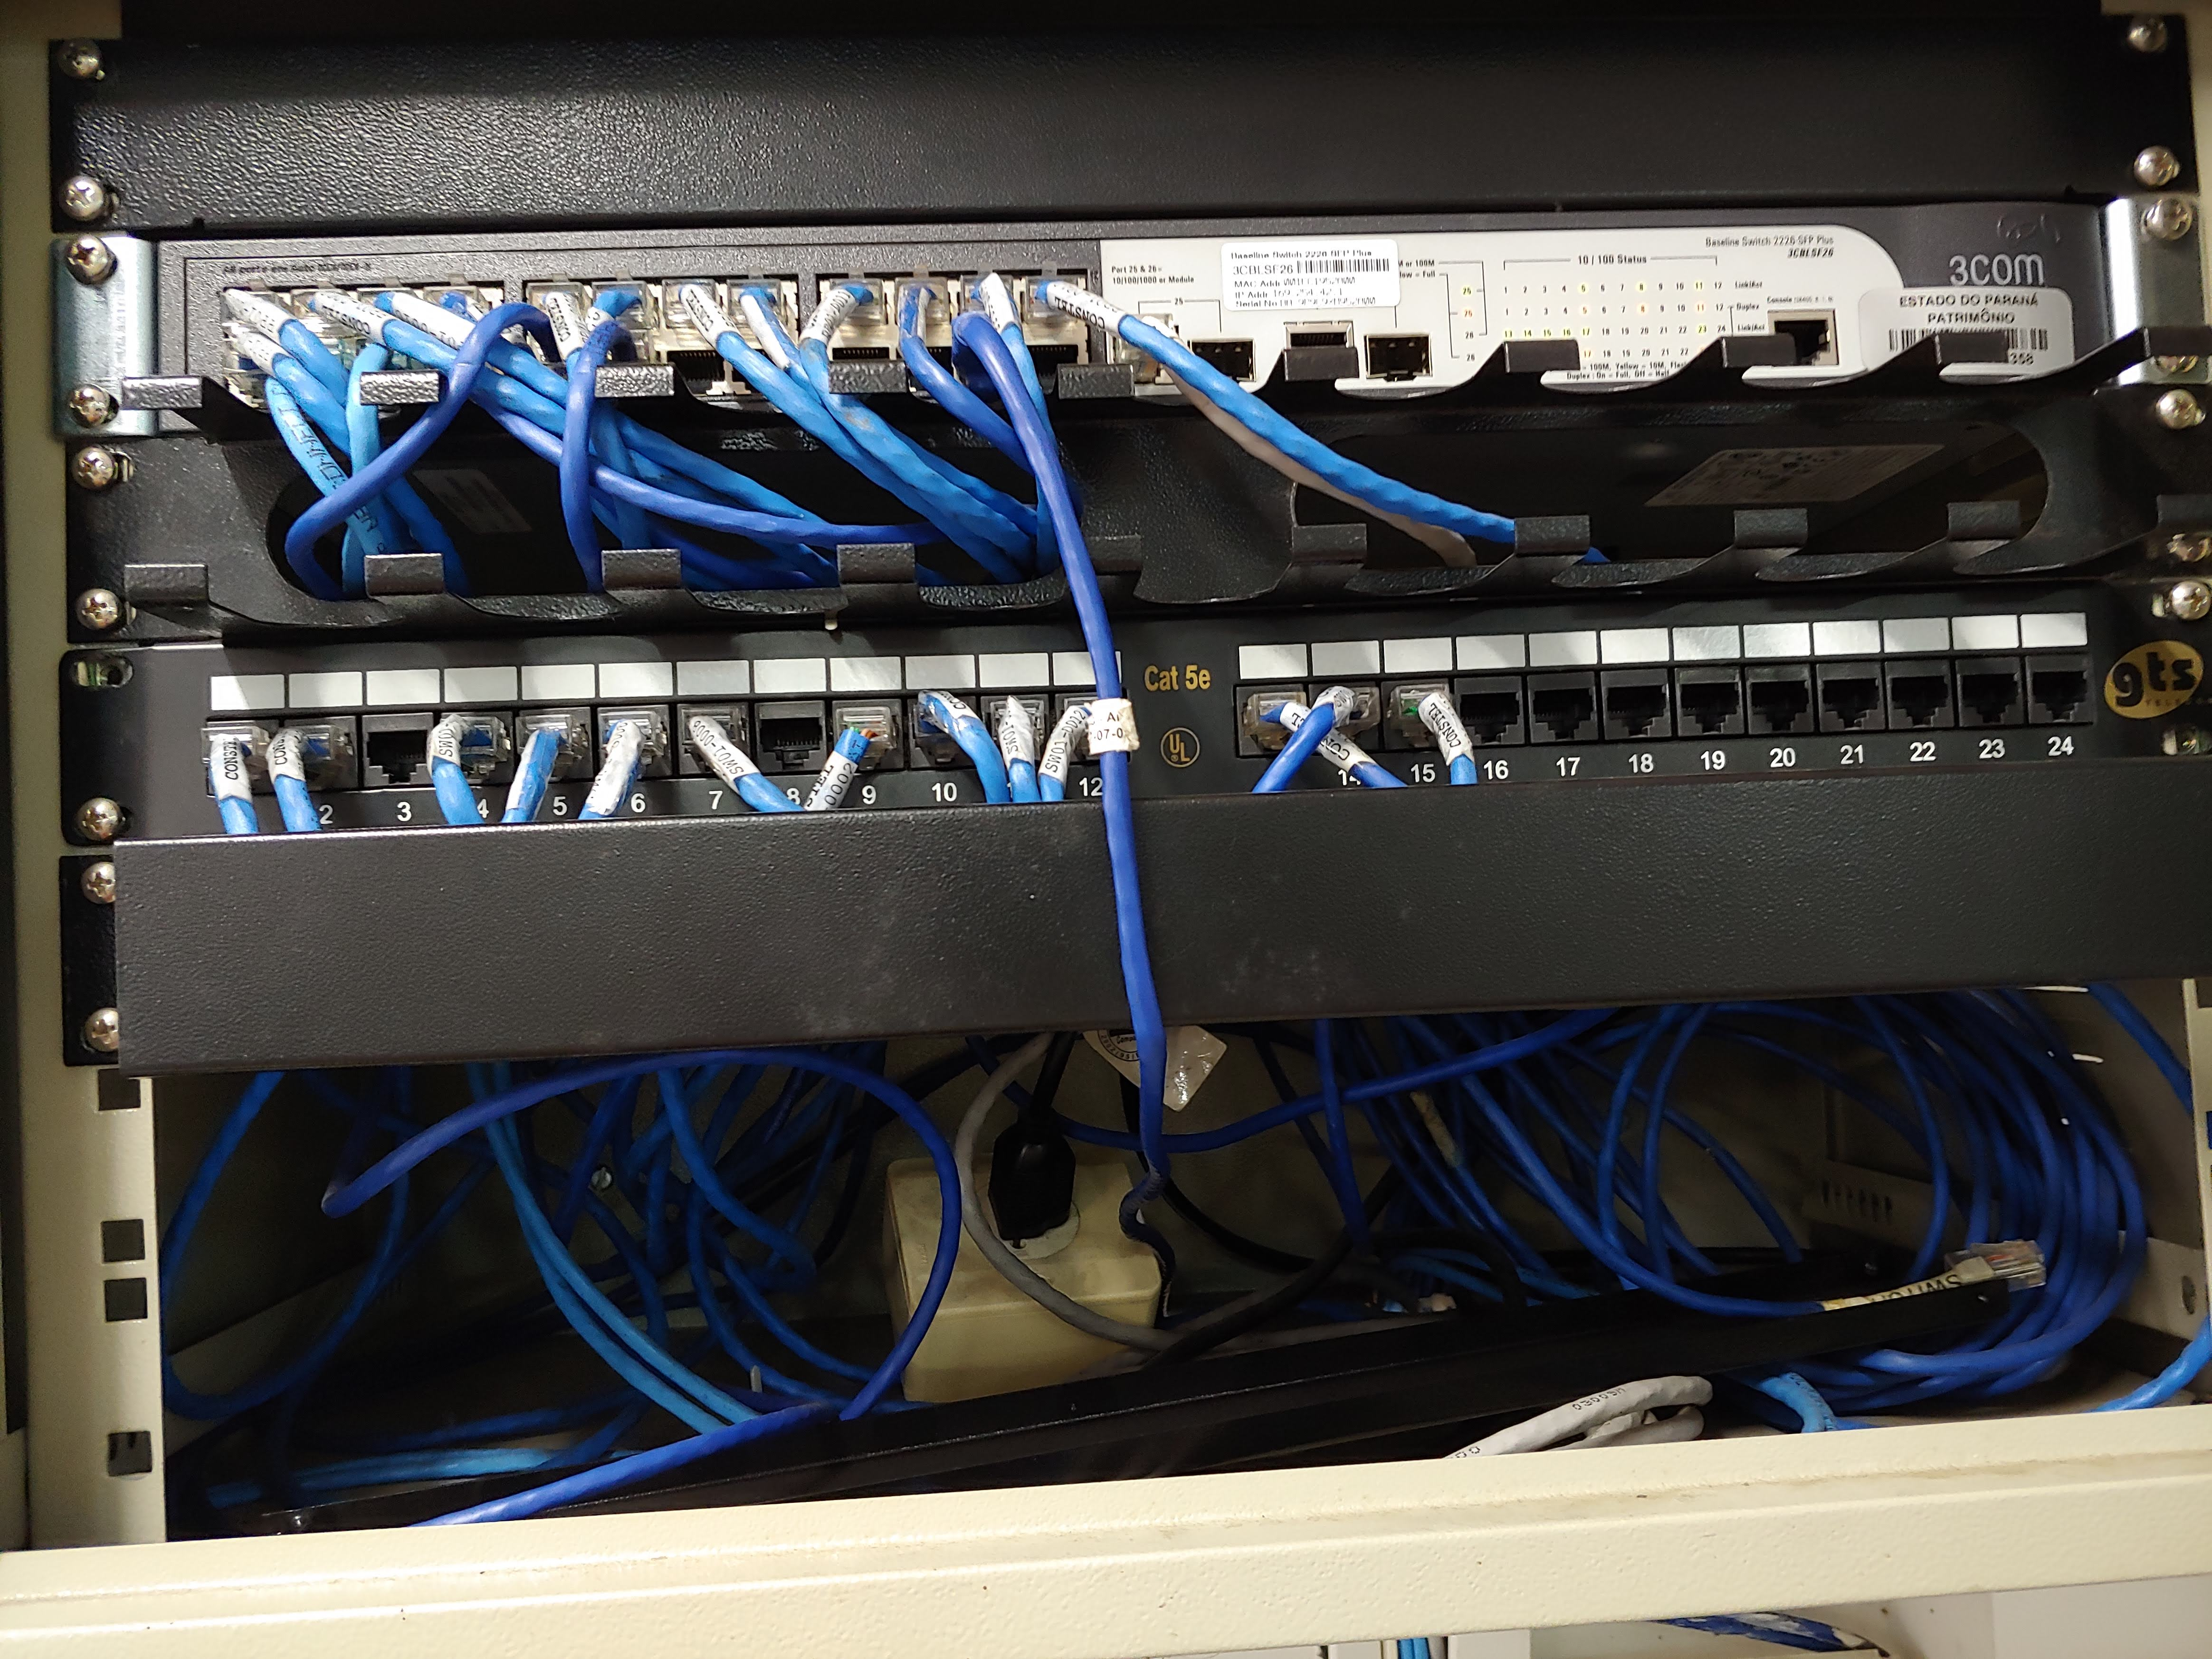
\includegraphics[width=0.7\textwidth]{figura11.jpg}
	\caption[Rack localizado no Setor de Fiscalização]{Rack localizado no Setor de Fiscalização}
	\label{figura11}
\end{figure}

\begin{figure}[h!]
	\centering
	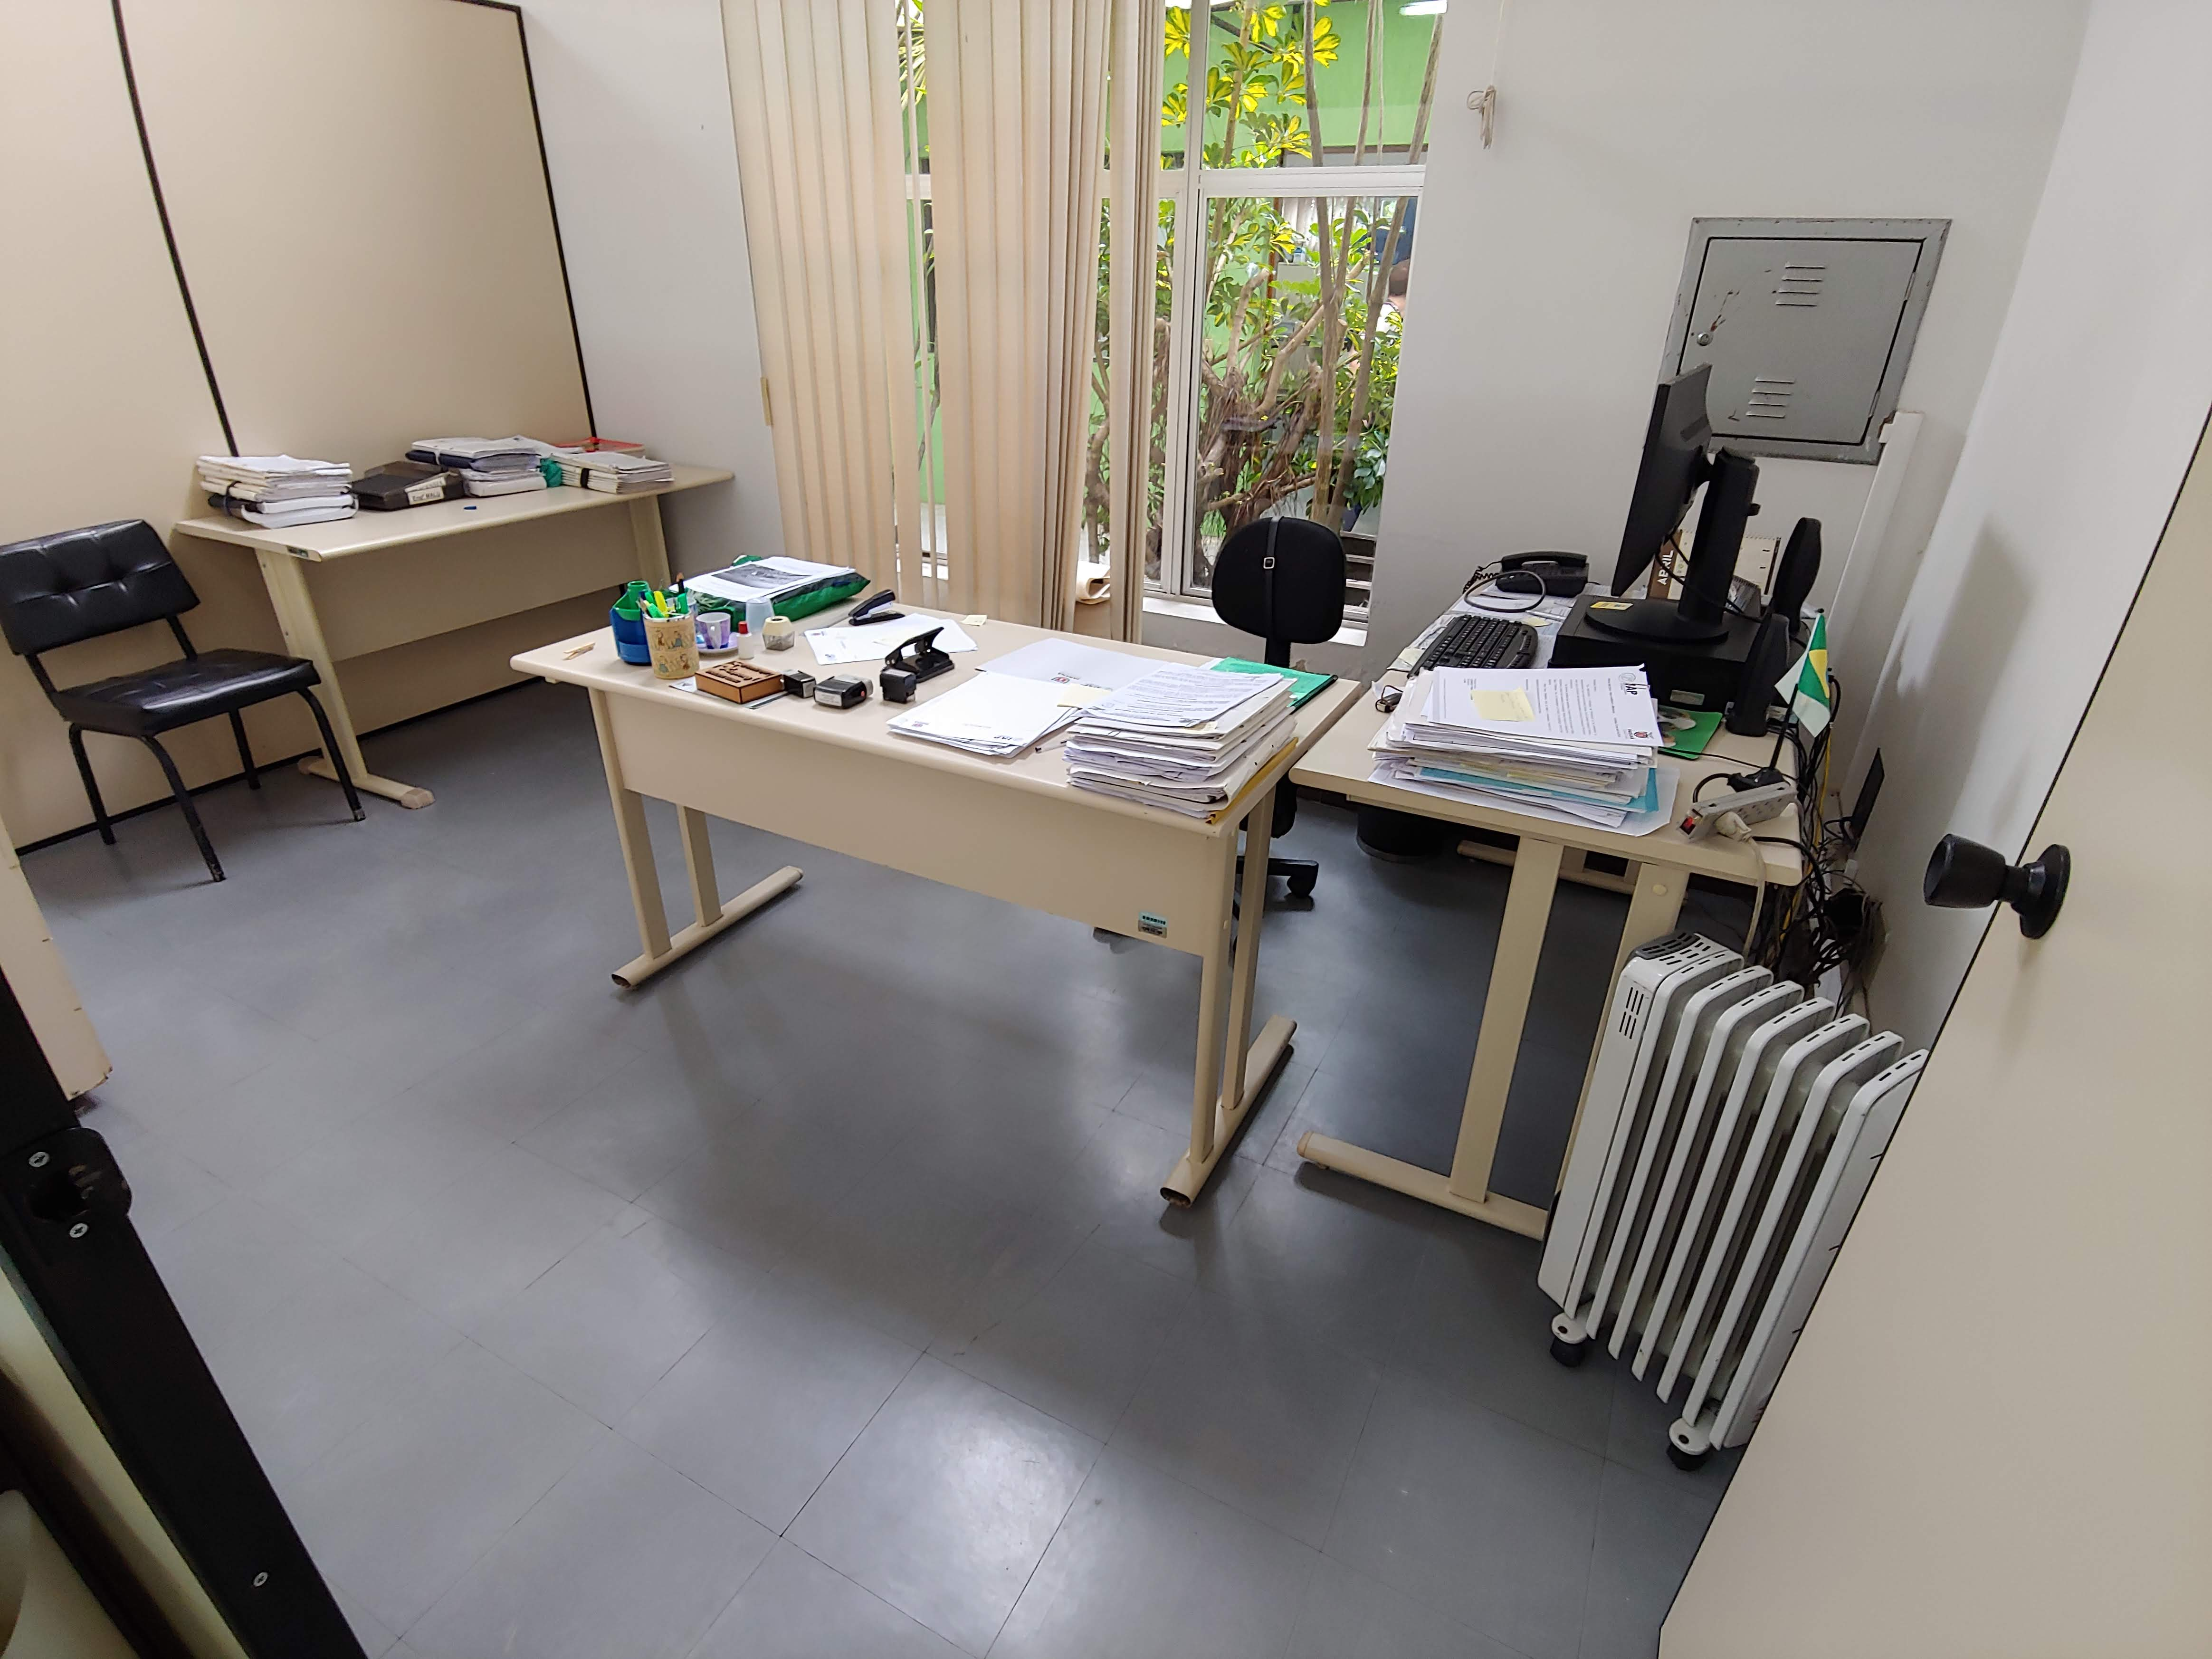
\includegraphics[width=0.7\textwidth]{figura12.jpg}
	\caption[Licenciamento Florestal]{Licenciamento Florestal}
	\label{figura12}
\end{figure}

\begin{figure}[h!]
	\centering
	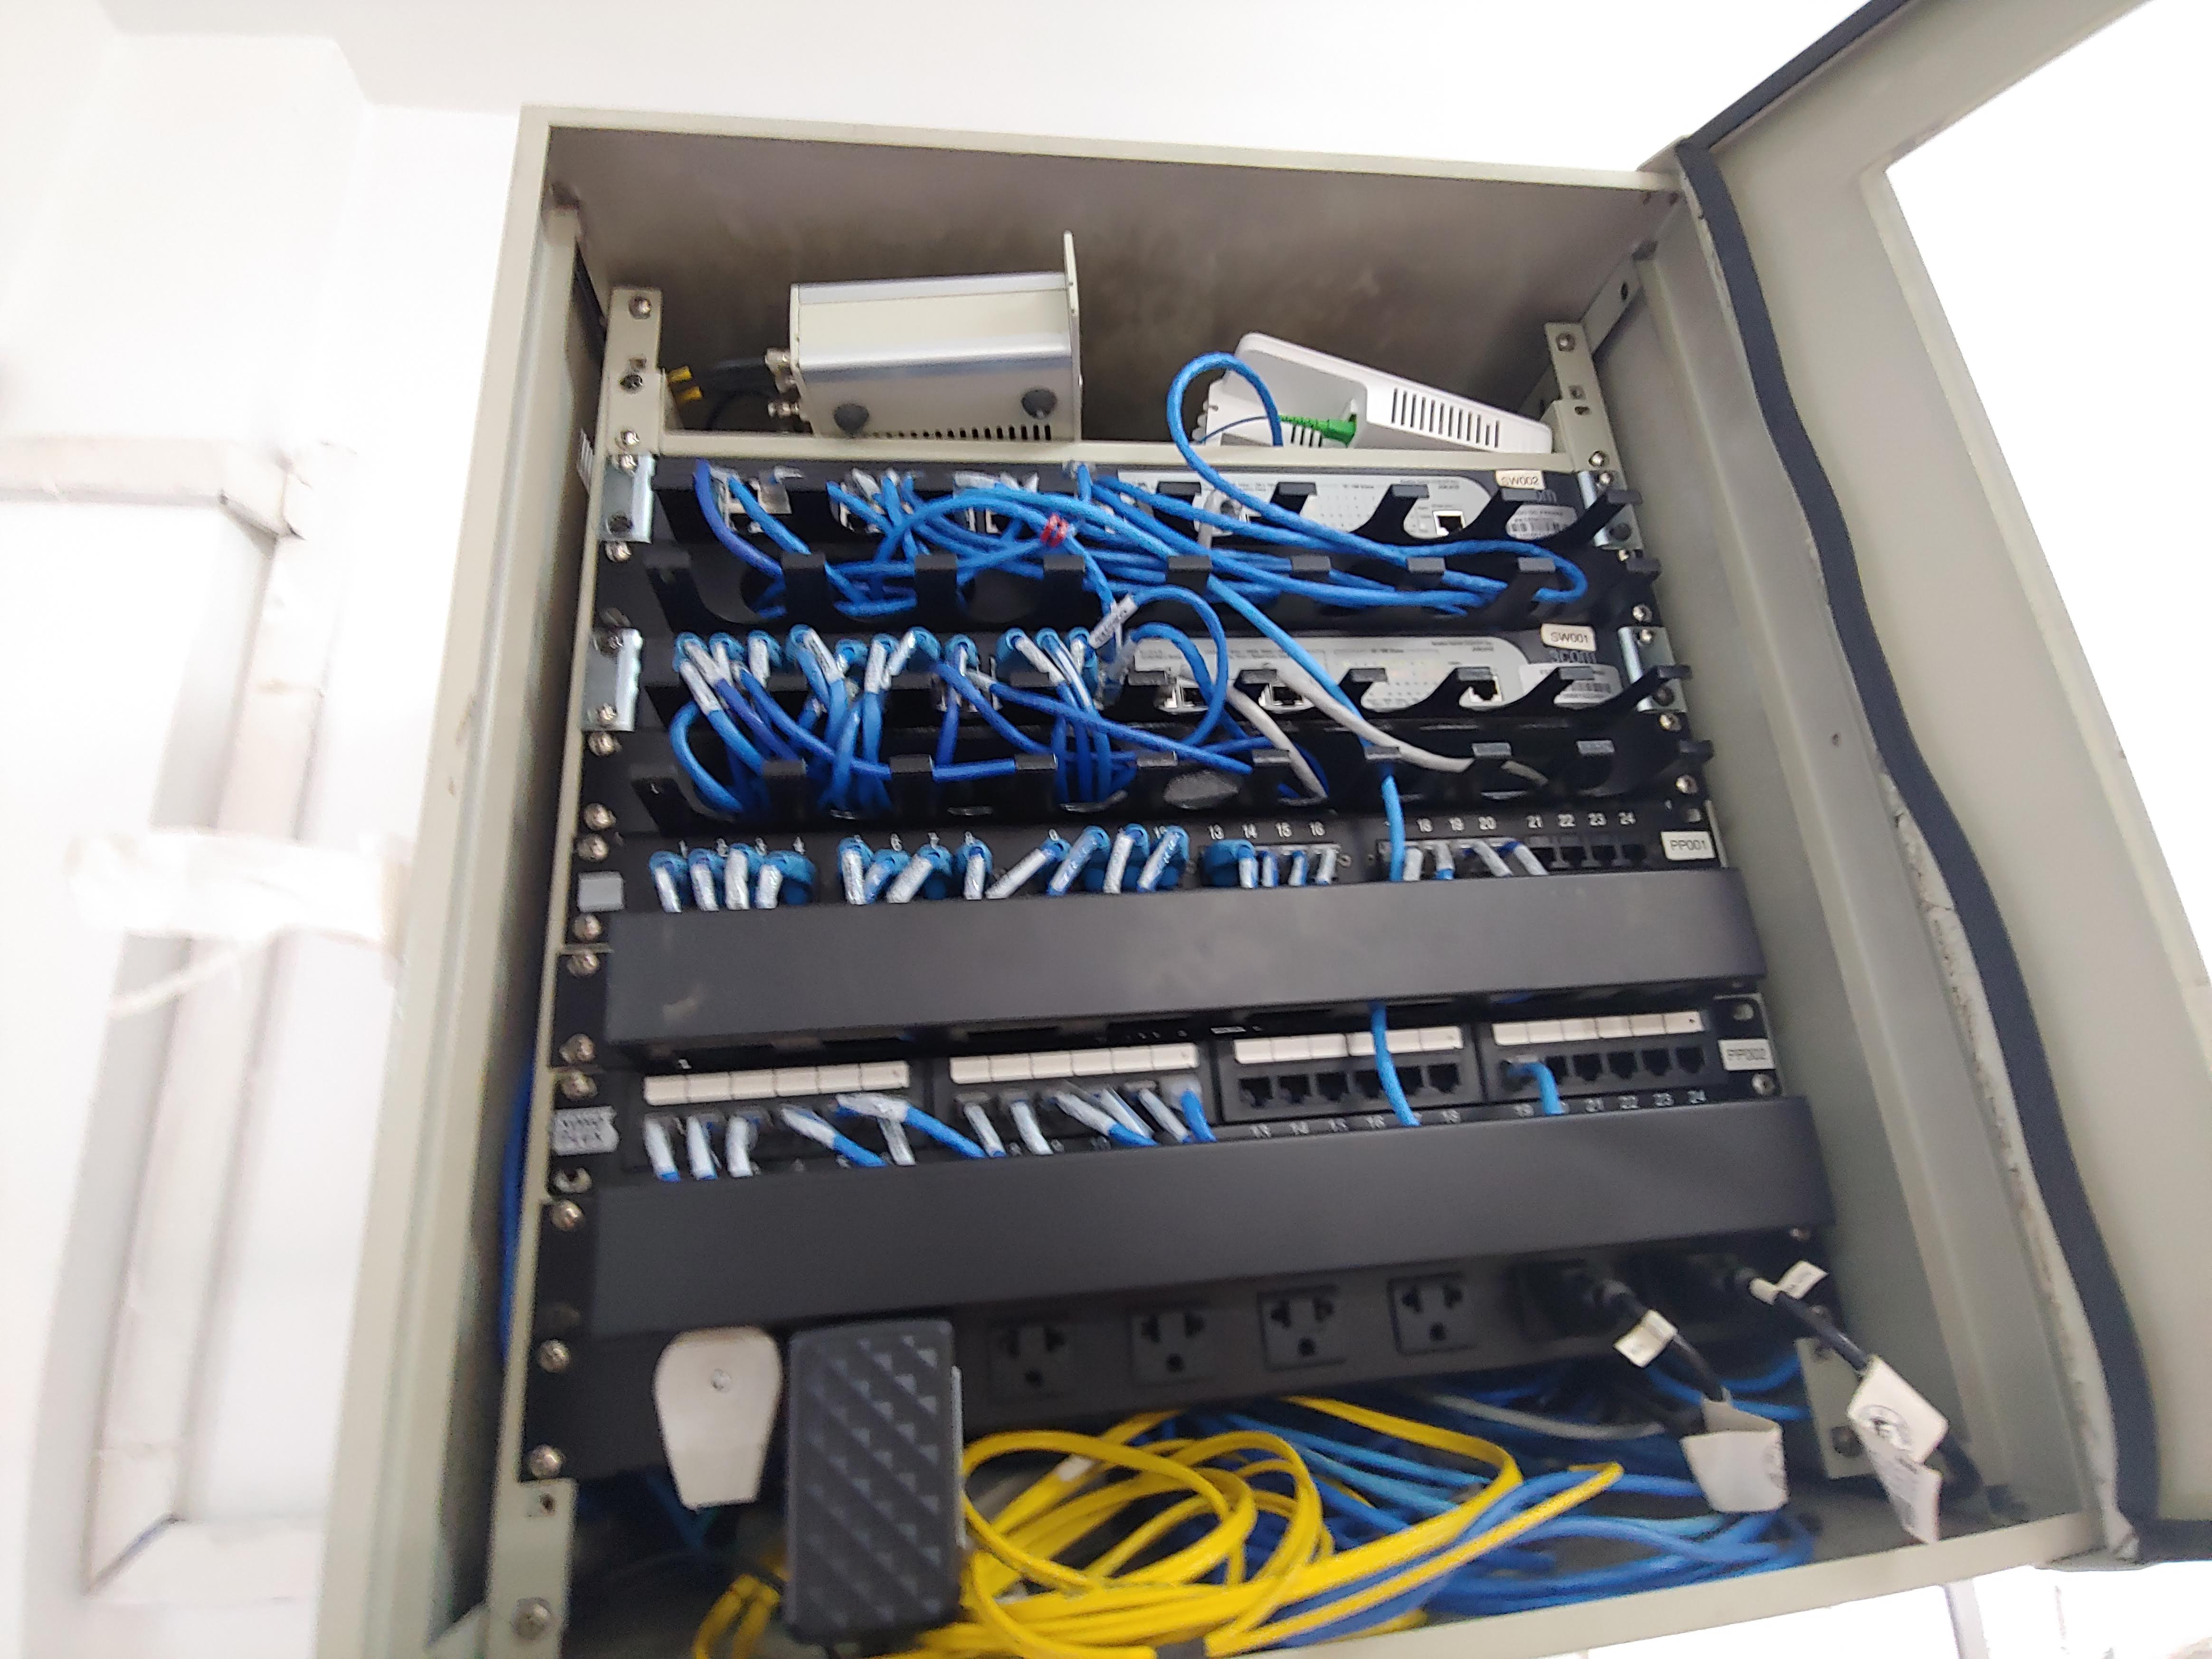
\includegraphics[width=0.7\textwidth]{figura14.jpg}
	\caption[Rack localizado no 1º Andar]{Rack localizado no 1º Andar}
	\label{figura14}
\end{figure}

\begin{figure}[h!]
	\centering
	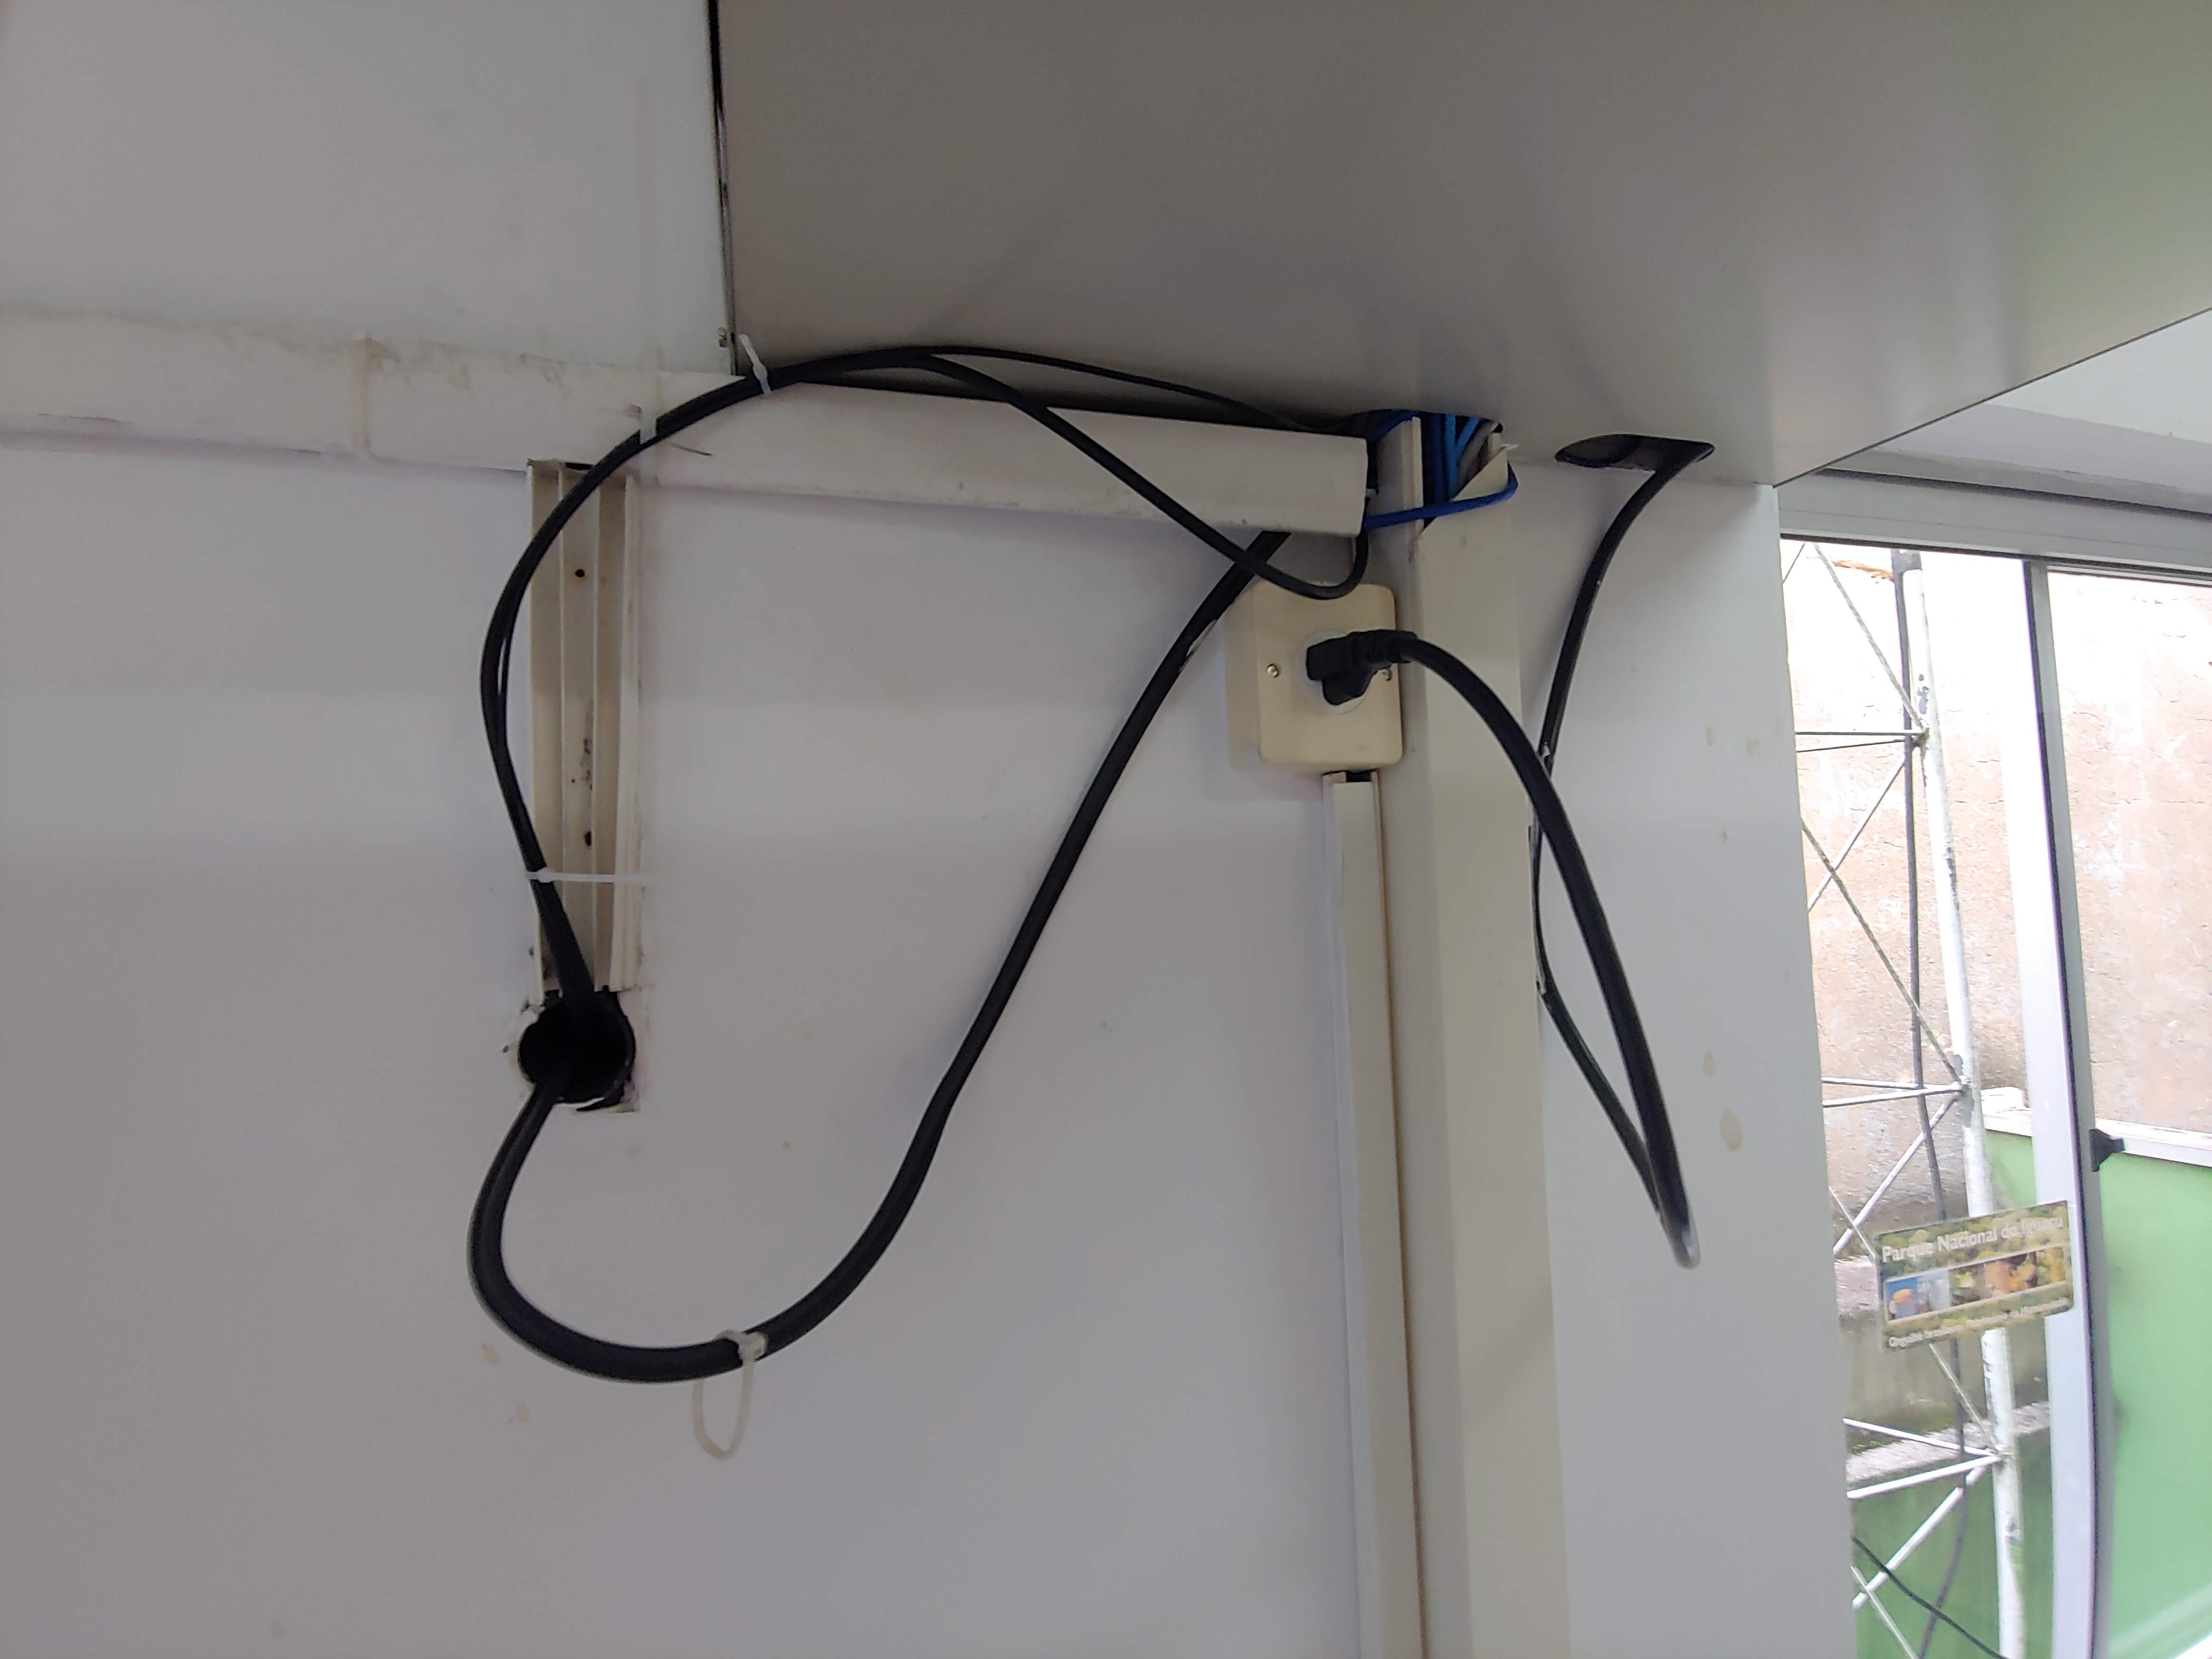
\includegraphics[width=0.7\textwidth]{figura13.jpg}
	\caption[Conexões elétricas do Rack]{Conexões elétricas do Rack}
	\label{figura13}
\end{figure}
\clearpage

\section{Requisitos}
\begin{itemize}
\item Rede escalável;
\item VLANs delimitando departamentos, bem como o tráfego de dados e voz;
\item Largura de banda capaz de atender demandas como: compartilhamentos de arquivos entre usuários, videoconferências, acesso remoto;
\item Servidor de arquivos;
\item Servidor de impressões;
\item Permitir que usuários de outras unidades possam se autenticar na rede local quando em trânsito;
\item Acesso e gerenciamento seguro de banco de dados;
\item Promover mecanismos que garanta a segurança da rede local;
\item Permitir o desenvolvimento e manutenção de serviços WEB, para permitir o acesso interno e externo às páginas e sistemas;
\item Analisar, avaliar, definir e adotar processos, técnicas e ferramentas para o desenvolvimento de software;
\item Administrar a infraestrutura de rede, diagnosticar problemas com seus componentes ou com o comportamento de computadores ligados à ela;
\item Instalação, configuração e manutenção dos sistemas computacionais (hardware e Software) da sede e das unidades descentralizadas, bem como prover treinamento, diagnosticar e resolver problemas inerentes aos sistemas computacionais.
\end{itemize}

\section{Usuários e Aplicativos}
O prédio é formado por dois andares. No térreo estão a Recepção, Licenciamento Florestal, Fiscalização, Arquivo e Combustível. No primeiro andar estão a Chefia, Arquivo, Licenciamento Industrial, Administrativo e Escritório Regional.\par
Por se tratar de um órgão público, ele depende de editais de seleção para aumento de seu quadro funcional, fato que não costuma ser constante.\par
Porém, devido a também possuir um caráter de instituto de pesquisa, atuando na área educacional, oferecendo curso de pós graduação stricto sensu (Mestrado em agricultura conservacionista), todo ano recebe cerca de 20 alunos novos.\par
Outro fator que pode refletir no aumento de usuários, são as contratações de consultores externos, mas que também são incluídos como usuários da rede.

\subsection{Usuários}
%Crie uma relação da quantidade, perfil de usuários de seu projeto.
\begin{table}[h!] % coloque h! para forcar a posicao
\onehalfspacing
\caption{Usuários e Aplicativos}
\vspace{0.5cm}
\centering
\label{tab2}
\resizebox{\textwidth}{!}{%
\begin{tabular}{|c|c|}
\hline
\textbf{Usuários}        & \textbf{Aplicativos}                                                 \\ \hline
Diretor                  & Microsoft Office, Videoconferência, Aplicações Web,                  \\ \hline
Recepcionista            & Microsoft Office, Controle de Acesso, Aplicações Web,                \\ \hline
Técnicos Administrativos & Microsoft Office, Videoconferência                                   \\ \hline
Pesquisadores            & Microsoft Office, Aplicações Web, Softwares de Análises Estatísticas \\ \hline
Alunos do Mestrado       & Microsoft Office, Aplicações Web, Softwares de Análises Estatísticas \\ \hline
\end{tabular}%
}

\end{table}

%\subsection{Aplicativos}
%Crie uma relação dos aplicativos e seus níveis críticos de uso.

\section{Estrutura predial existente}
A estrutura predial existente está demonstrada pelas plantas nas figuras \ref{figura1} e \ref{figura2}.
%\
%\textbf{A T E N Ç Ã O - A C H T U N G !}
%\\
%Daqui está faltando uma pequena explicação para "encher linguiça"... Digam aqui, literalmente, como está a estrutura predial existente. Época de construção, como está a conservação, de que alvenaria é feita, se é quebrável, se é fácil trabalhar com essa estrutura... 
%\
%Usem vertical space  para espaçar os parágrafos.
%\
%Enfim, explicar até o fim dessa página, textualmente, um pouco das duas plantas - em que software foi desenhado, as medidas maiores delas, etc.
%Explique aqui a planta física dos prédios
%Pode ser anexada, em escala ou não.

%Deve conter uma descrição geral, indicando a possível distância entre os pontos de rede e restrições de instalação.
A estrutura do IAP é dividida em duas plantas, sendo a Térreo e 1º Andar; no Térreo estão os setores: Recepção, Fiscalização, Licenciamento Florestal, SI, Arquivo e Combustível. No 1º Andar estão: Chefia, Arquivo, Licenciamento Industrial, Administrativo e Escritório Regional.\par
Construção aproximadamente de 550m². Alvenaria do tipo vedação, maior durabilidade, é oferecida uma flexibilidade e versatilidade maior, seus materiais de construção são mais baratos, é mais aceitável por ser mais comum, o custo-benefício em relação a todos os materiais disponíveis para vedação é melhor, acessível à futuras reformas.A construção inicial não era designada ao instituto que posteriormente foi comprada para a atual instalação, tanto que compartilha alguns ambientes com outro órgão governamental, logo, os ambientes são irregulares, as divisões dos setores são por \textit{drywall}, adaptados o cabeamento lógico e elétrico, portanto, se necessário é possível e fácil a alteração do layout dos ambientes.\par
As plantas baixas foram desenvolvidas pelo \href{http://www.sweethome3d.com/pt/}{Sweet Home 3D} - SH3D, as figuras \ref{figura22} e \ref{figura23} são dois exemplos das plantas em 3D.

\clearpage
%==============================A3 INICIO===========================
\clearpage 
\thispagestyle{plain}
\KOMAoptions{paper=a3, paper=landscape, DIV=20}
\recalctypearea
\begin{figure}
	\noindent\makebox[\textwidth][c]{
		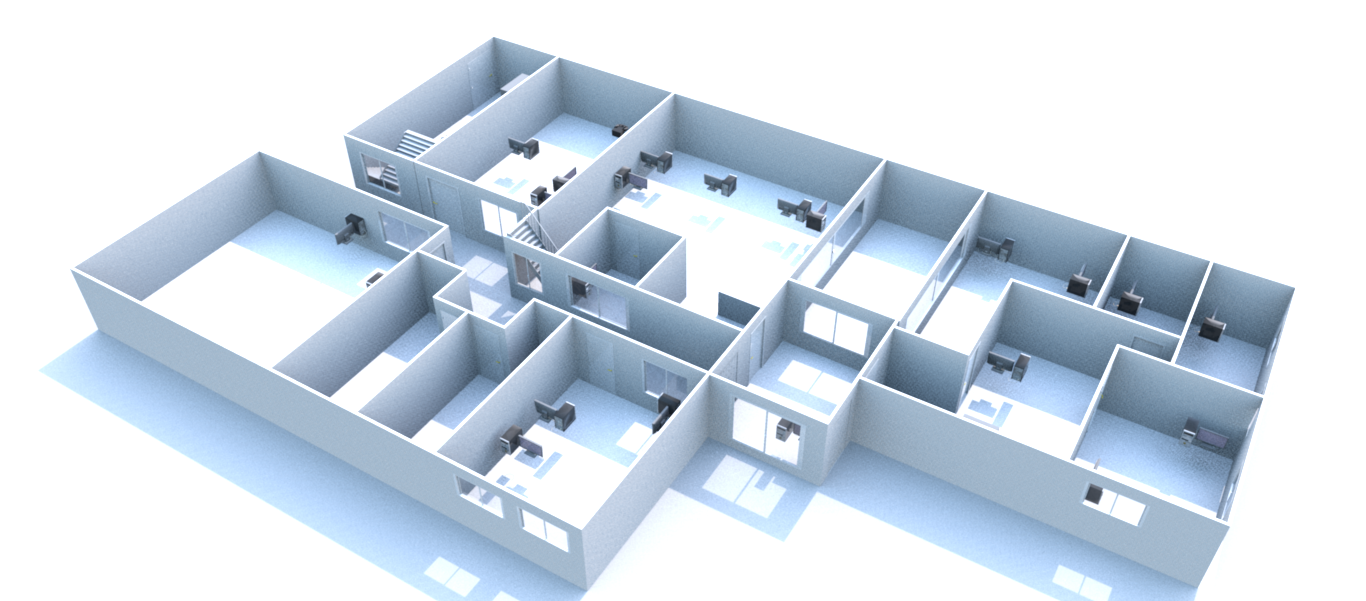
\includegraphics[width=\textwidth]{IAP_terreo}
	}
	\caption[Planta Baixa Térreo SH3D]{Planta Baixa Térreo SH3D}
	\label{figura22}
\end{figure}

%REVERTER

\clearpage
\KOMAoptions{paper=a4, paper=portrait, DIV=15}
\recalctypearea
%==============================A3 FIM=========================== 
\iffalse
\begin{figure}[h!]
	\centering
	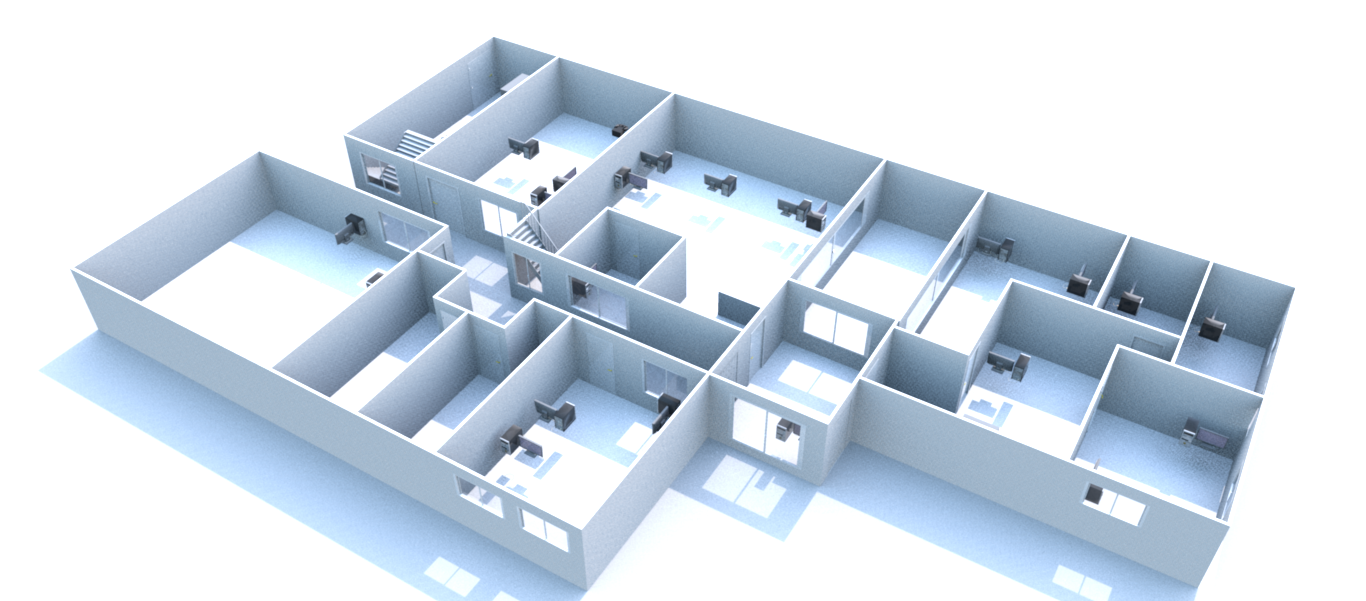
\includegraphics[width=\textwidth]{IAP_terreo.png}
	\caption[Planta Baixa Térreo SH3D]{Planta Baixa Térreo SH3D}
	\label{figura22}
\end{figure}
\fi
%==============================A3 INICIO===========================
\clearpage 
\thispagestyle{plain}
\KOMAoptions{paper=a3, paper=landscape, DIV=20}
\recalctypearea
\begin{figure}
	\noindent\makebox[\textwidth][c]{
		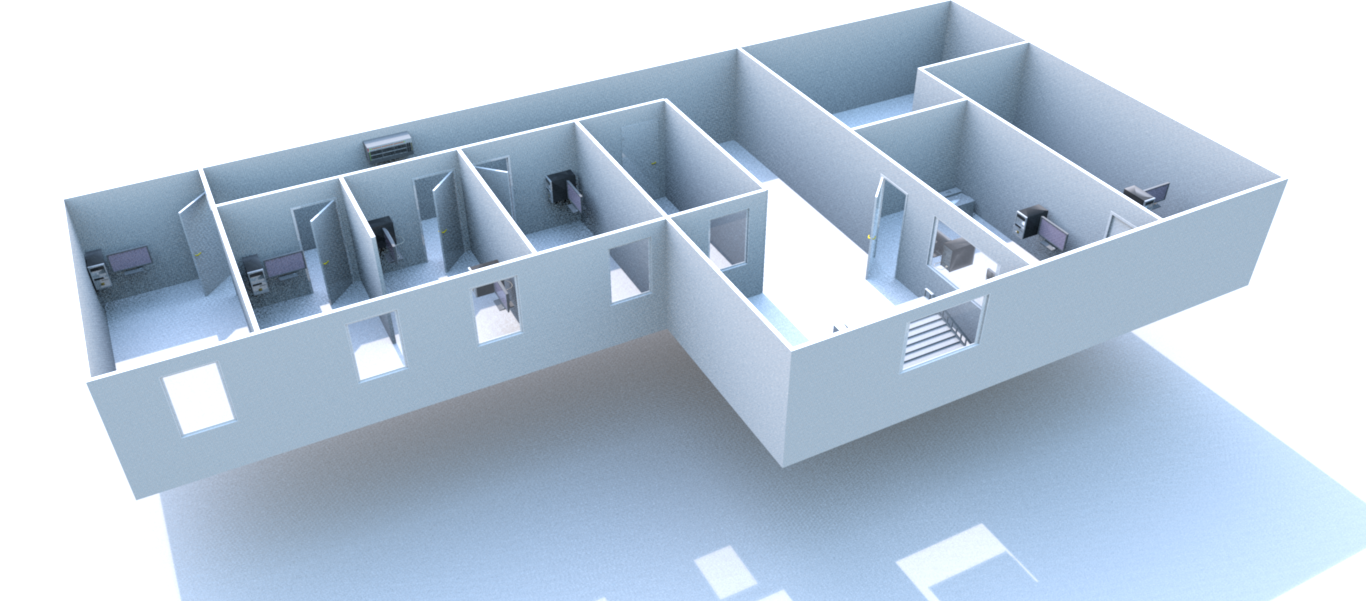
\includegraphics[width=\textwidth]{IAP_1andar}
	}
	\caption[Planta Baixa 1º Andar SH3D]{Planta Baixa 1º Andar SH3D}
	\label{figura23}
\end{figure}

%REVERTER

\clearpage
\KOMAoptions{paper=a4, paper=portrait, DIV=15}
\recalctypearea
%==============================A3 FIM=========================== 

%==============================A3 INICIO===========================
\clearpage 
\thispagestyle{plain}
\KOMAoptions{paper=a3, paper=landscape, DIV=20}
\recalctypearea
\begin{figure}
	\noindent\makebox[\textwidth][c]{
		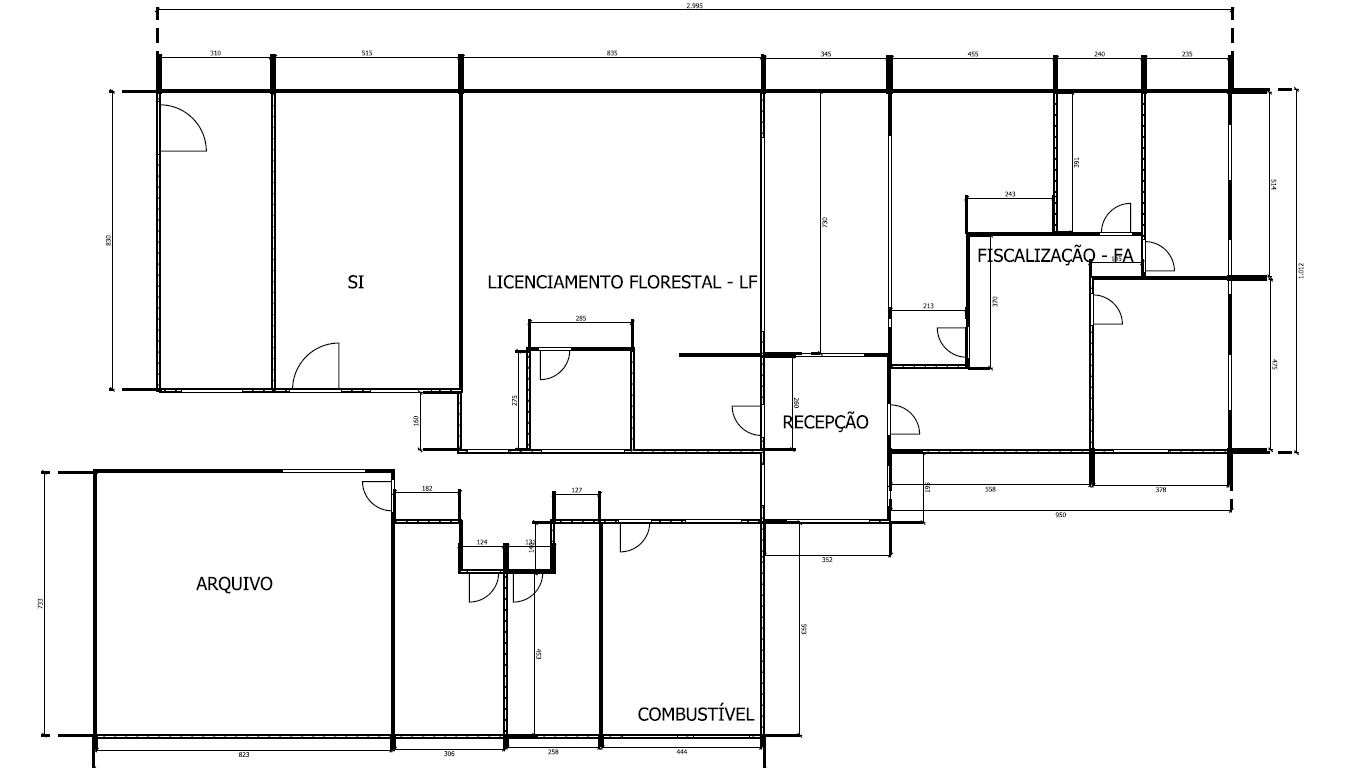
\includegraphics[width=\textwidth]{figura1}
	}
	\caption[Planta Baixa Térreo]{Planta Baixa Térreo}
	\label{figura1}
\end{figure}

%REVERTER

\clearpage
\KOMAoptions{paper=a4, paper=portrait, DIV=15}
\recalctypearea
%==============================A3 FIM=========================== 
\iffalse
\begin{figure}[h!]
	\centering
	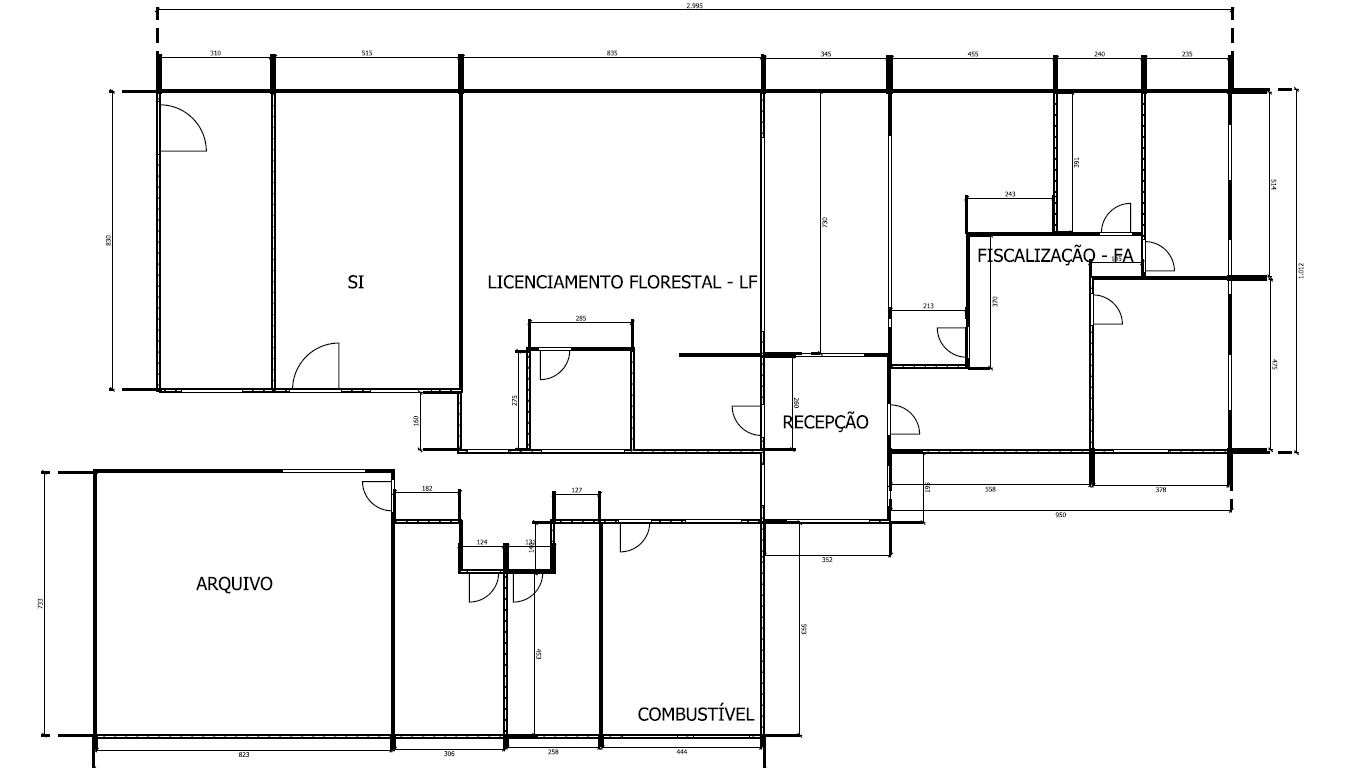
\includegraphics[width=\textwidth]{figura1.png}
	\caption[Planta Baixa Térreo]{Planta Baixa Térreo}
	\label{figura1}
\end{figure}
\fi
%==============================A3 INICIO===========================
\clearpage 
\thispagestyle{plain}
\KOMAoptions{paper=a3, paper=landscape, DIV=20}
\recalctypearea
\begin{figure}
	\noindent\makebox[\textwidth][c]{
		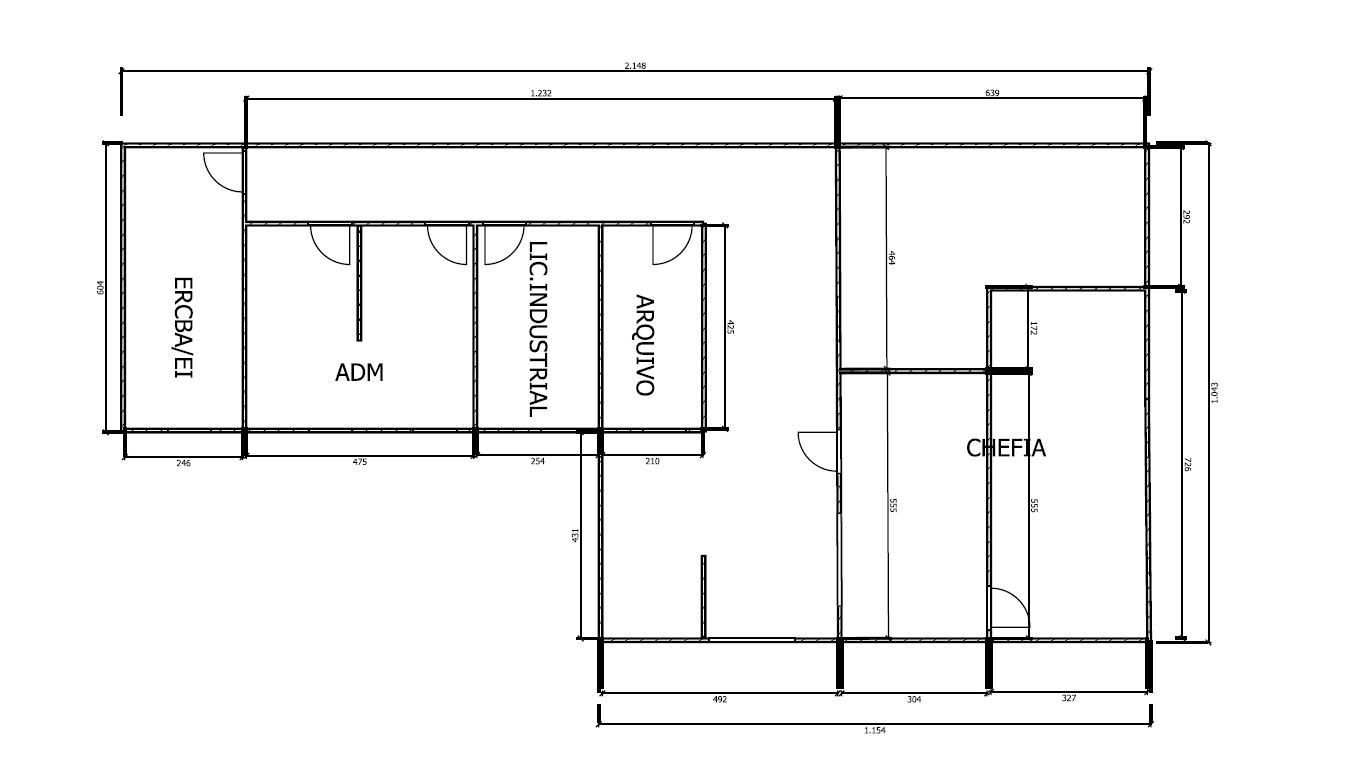
\includegraphics[width=\textwidth]{figura2}
	}
	\caption[Planta baixa 1º andar IAP]{Planta baixa 1º andar IAP}
	\label{figura2}
\end{figure}

%REVERTER

\clearpage
\KOMAoptions{paper=a4, paper=portrait, DIV=15}
\recalctypearea
%==============================A3 FIM=========================== 
\begin{figure}[h!]
	\centering
	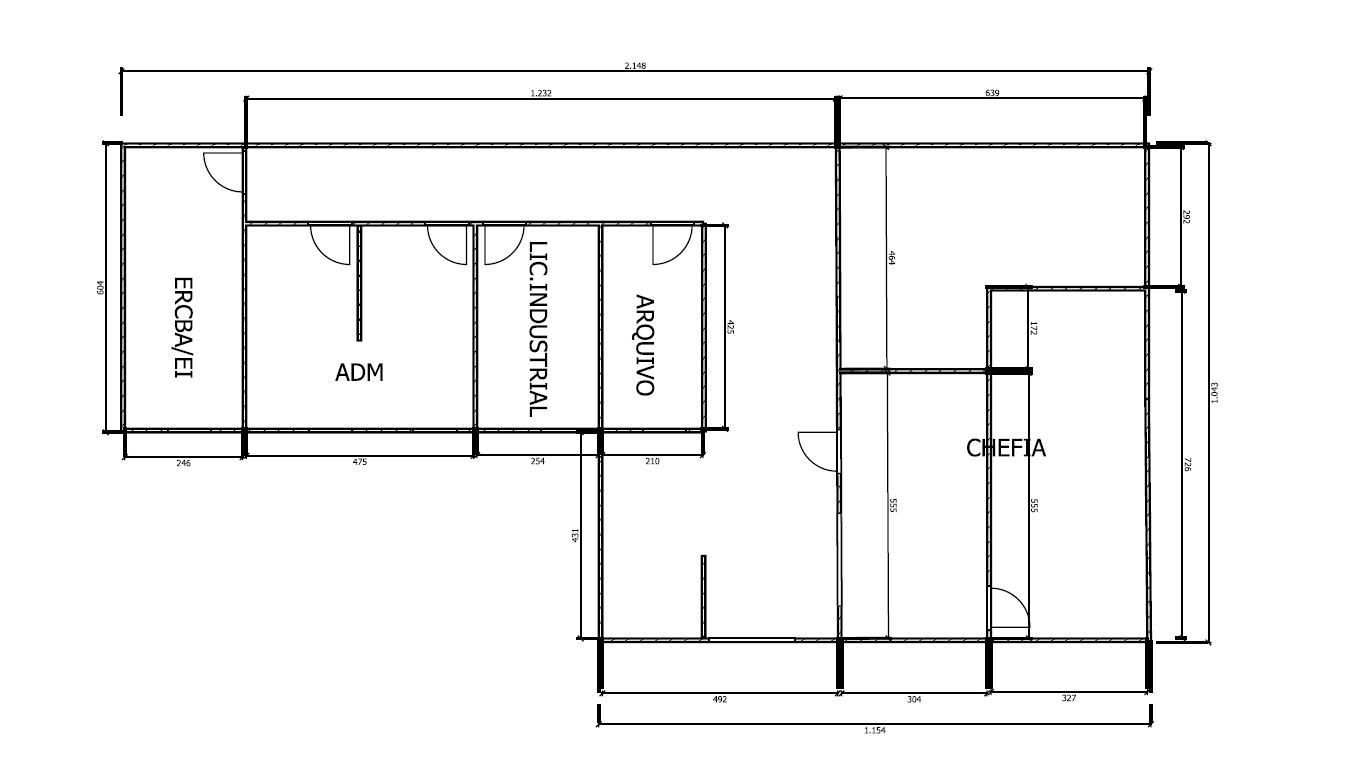
\includegraphics[width=\textwidth]{figura2.png}
	\caption[Planta baixa 1º andar IAP]{Planta baixa 1º andar IAP}
	\label{fig:figura2}
\end{figure}
\section{Planta Lógica - Elementos estruturados}

\subsection{Estado atual}
%Deve ter a planta atual, se for o caso

O estado atual está demonstrada pelas plantas das figuras \ref{figura3}, \ref{figura4}\, \ref{figura5}, e \ref{figura6}.\par
Para o desenvolvimento das plantas, foi utilizado o software Visio da Microsoft, com base nas plantas baixas criadas anteriormente no Sweet Home 3D.\par
A partir do Distribuidor Geral de Telecomunicações, figura \ref{figura4}, cada ambiente possui um ponto de conexão primário, no propósito de redução e flexibilização da comunicação interna.\par
No térreo estão distribuídos 23 estações de trabalho e uma impressora de rede.\par
O cabeamento é efetuado pelo forro do teto, evitando perfuração nas paredes (visto que a construção é antiga), e estendidos por calhas de PVC no cabeamento nas paredes e rodapés.\par
No primeiro andar, figura \ref{figura6}, a topologia é similar ao térreo, onde a conexão de entrada é pelo AT (sendo este possuindo dois switches) distribuindo o sinal cabeado pelos ambientes.\par
No primeiro andar, consta dez estações de trabalho e uma impressora conectada diretamente a rede.
%
%\
%\textbf{A T E N Ç Ã O - A C H T U N G !}
%\\
%Daqui está faltando uma pequena explicação para "encher linguiça"... Digam aqui, literalmente, como se dão as 4 figuras seguintes. Façam 1 parágrafo para cada, explicando que software foi usado, e algumas coisas técnicas: Exemplo: vemos na figura 4 que do switch, saem os cabos para elevações e canaletas, etc, etc.

%==============================A3 INICIO===========================
\clearpage 
\thispagestyle{plain}
\KOMAoptions{paper=a3, paper=landscape, DIV=20}
\recalctypearea
\begin{figure}
	\noindent\makebox[\textwidth][c]{
		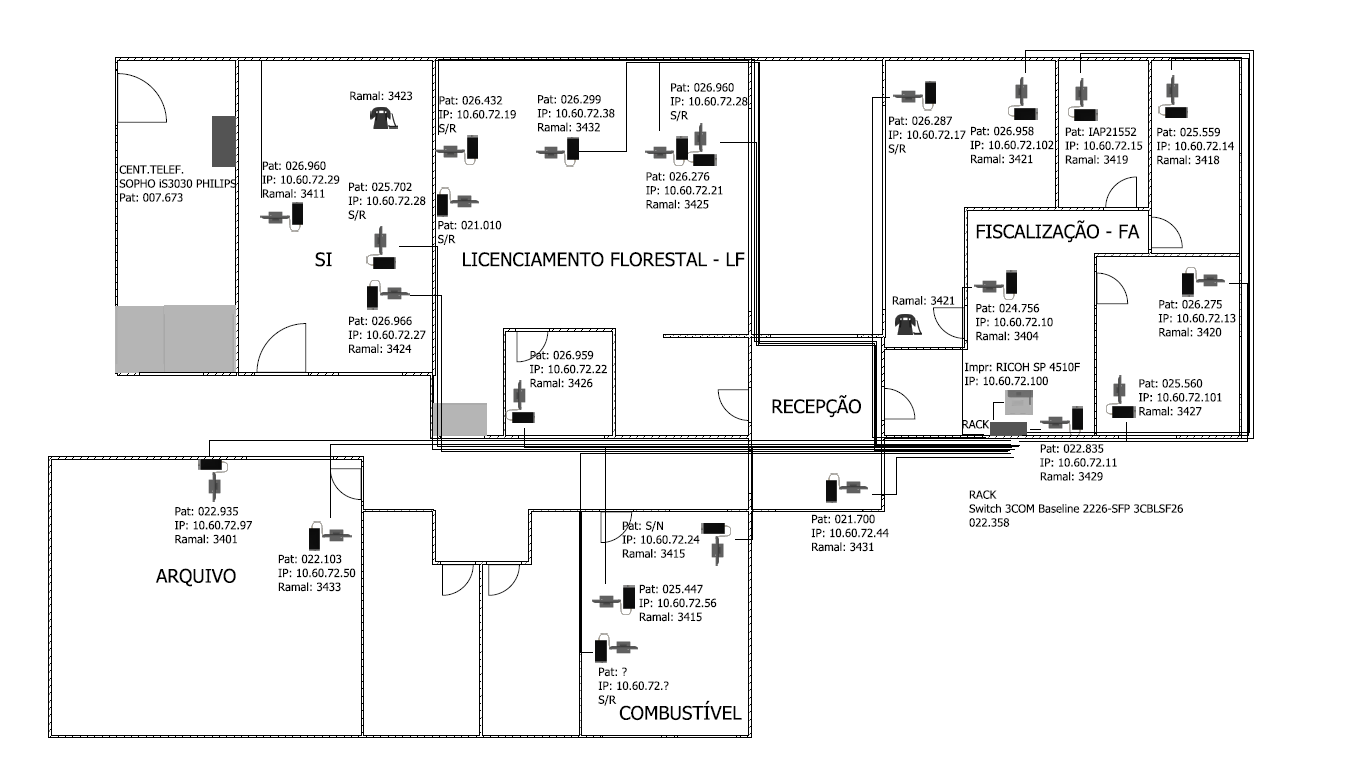
\includegraphics[width=\textwidth]{figura3}
	}
		\caption[Estado Atual - Posições das Áreas de Trabalho - Térreo]{Estado Atual - Posições das Áreas de Trabalho - Térreo}
	\label{figura3}
\end{figure}

%REVERTER

\clearpage
\KOMAoptions{paper=a4, paper=portrait, DIV=15}
\recalctypearea
%==============================A3 FIM===========================
\iffalse
\begin{figure}[h!]
	\centering
	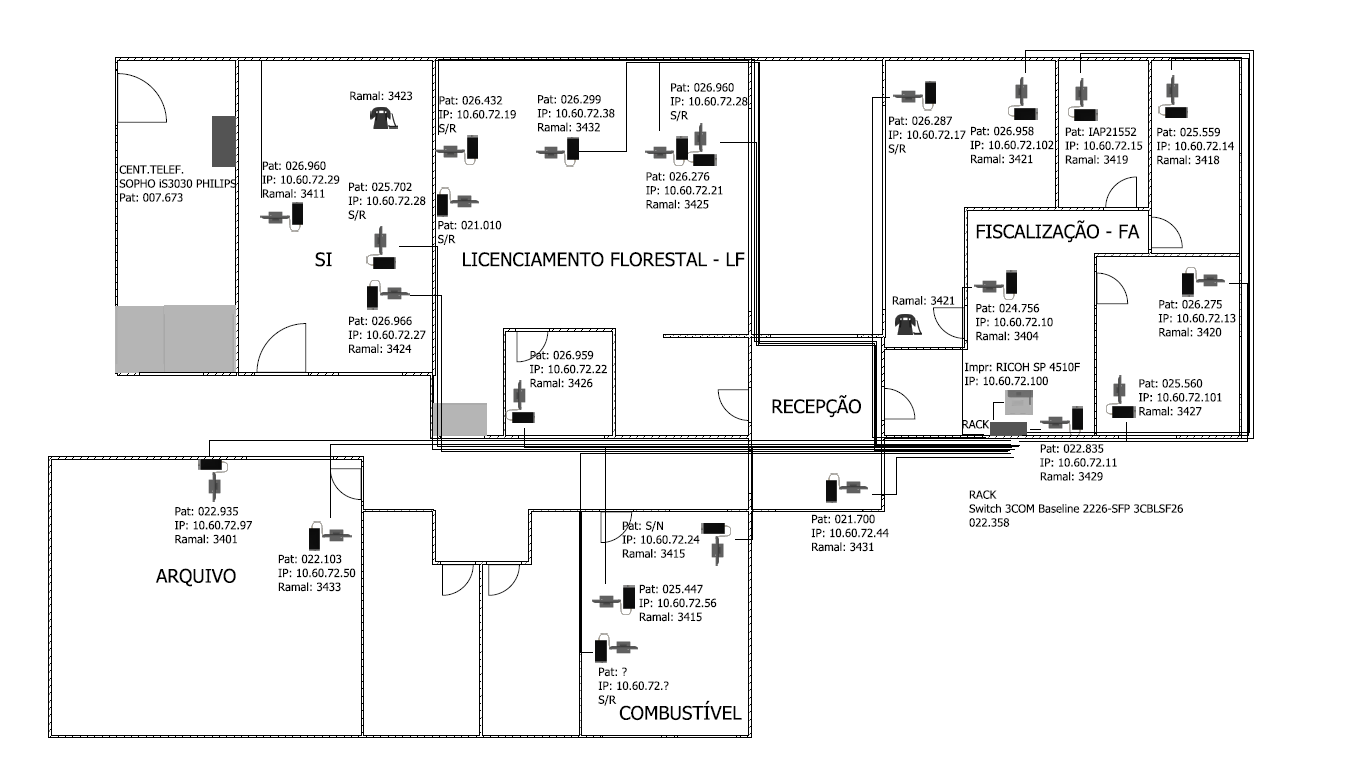
\includegraphics[width=\textwidth]{figura3.png}
	\caption[Estado Atual - Posições das Áreas de Trabalho - Térreo]{Estado Atual - Posições das Áreas de Trabalho - Térreo}
	\label{figura3}
\end{figure}
\fi
%==============================A3 INICIO===========================
\clearpage 
\thispagestyle{plain}
\KOMAoptions{paper=a3, paper=landscape, DIV=20}
\recalctypearea
\begin{figure}
	\noindent\makebox[\textwidth][c]{
		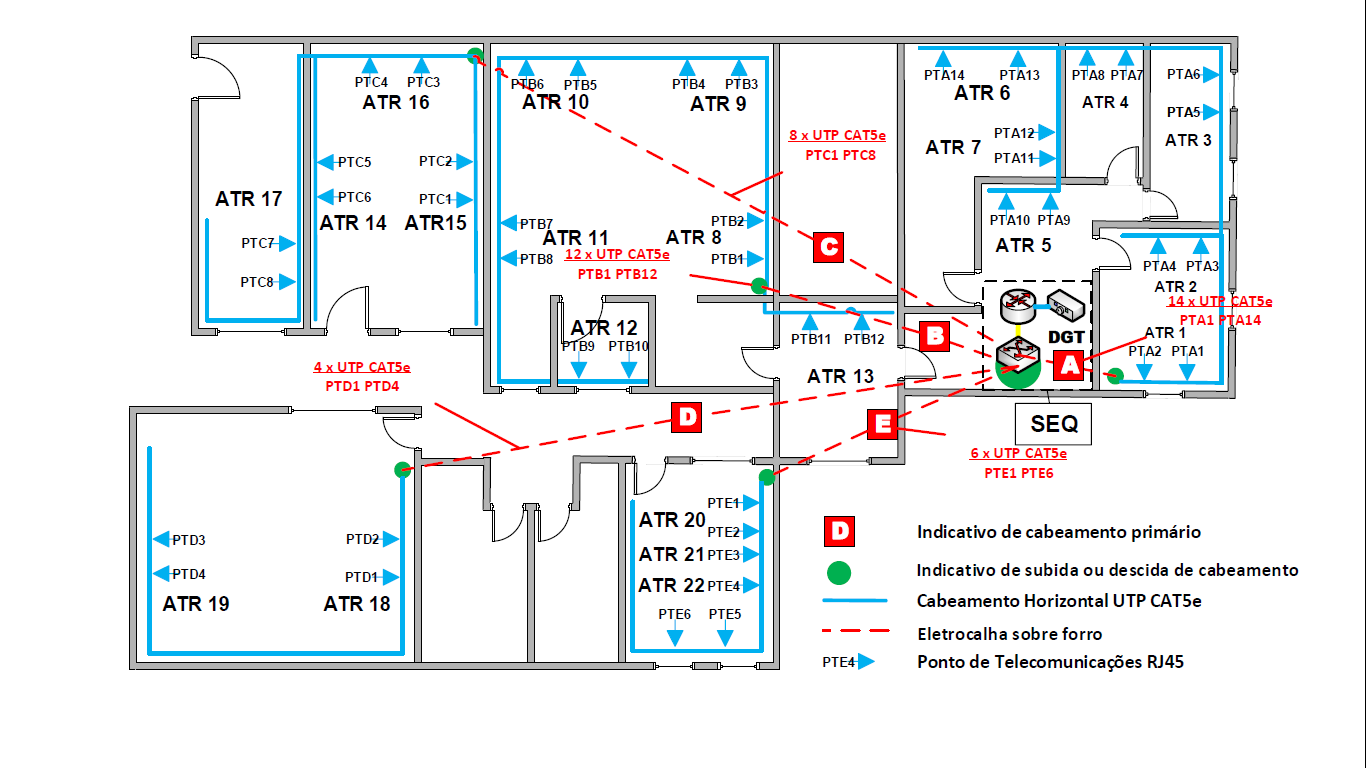
\includegraphics[width=\textwidth]{figura4}
	}
\caption[Estado Atual - Distribuição Cabeamento Horizontal/Backbone - Térreo]{Estado Atual - Distribuição Cabeamento Horizontal/Backbone - Térreo}
	\label{figura4}
\end{figure}

%REVERTER

\clearpage
\KOMAoptions{paper=a4, paper=portrait, DIV=15}
\recalctypearea
%==============================A3 FIM===========================
\iffalse
\begin{figure}[h!]
	\centering
	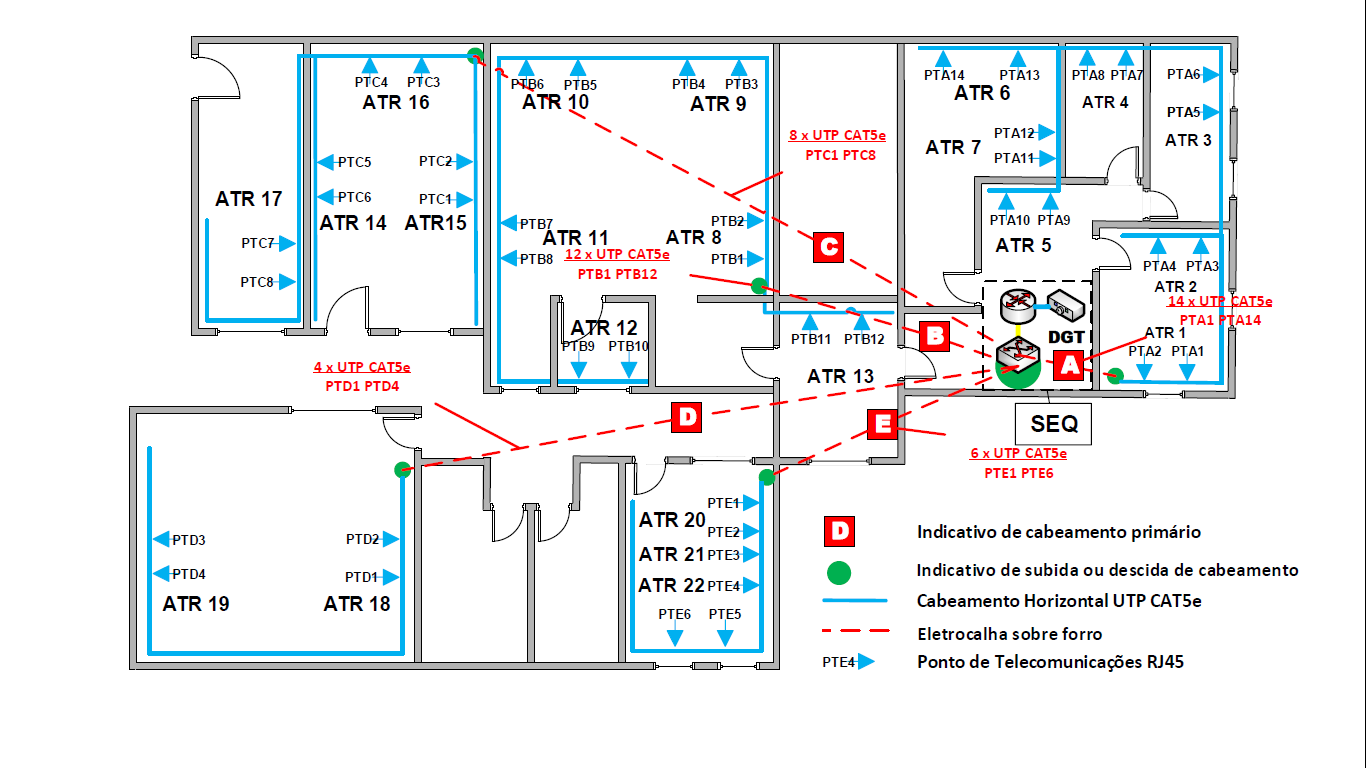
\includegraphics[width=\textwidth]{figura4.png}
	\caption[Estado Atual - Distribuição Cabeamento Horizontal/Backbone - Térreo]{Estado Atual - Distribuição Cabeamento Horizontal/Backbone - Térreo}
	\label{figura4}
\end{figure}
\fi
%==============================A3 INICIO===========================
\clearpage 
\thispagestyle{plain}
\KOMAoptions{paper=a3, paper=landscape, DIV=20}
\recalctypearea
\begin{figure}
	\noindent\makebox[\textwidth][c]{
		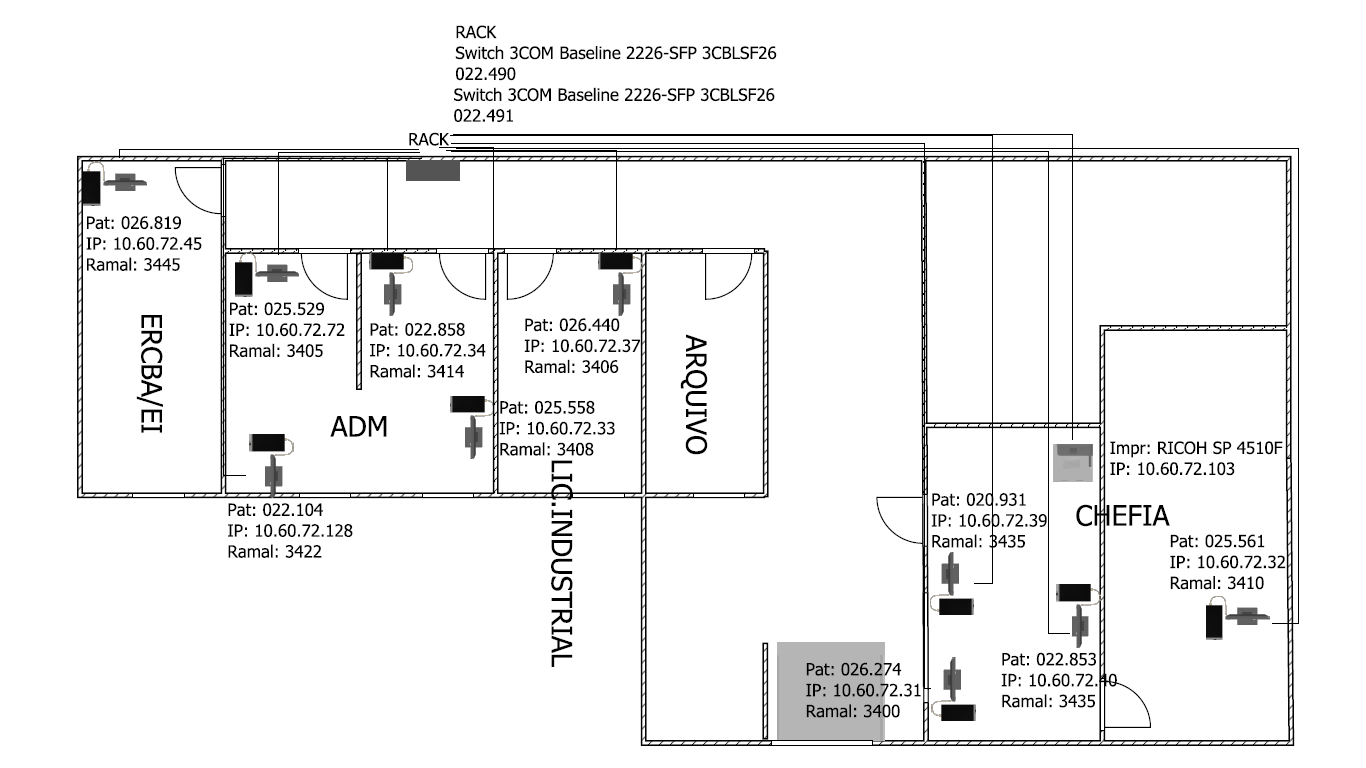
\includegraphics[width=\textwidth]{figura5}
	}
\caption[Trabalho - Térreo]{Estado Atual - Posições das Áreas de Trabalho - Térreo}
	\label{figura5}
\end{figure}

%REVERTER

\clearpage
\KOMAoptions{paper=a4, paper=portrait, DIV=15}
\recalctypearea
%==============================A3 FIM===========================
\iffalse
\begin{figure}[h!]
	\centering
	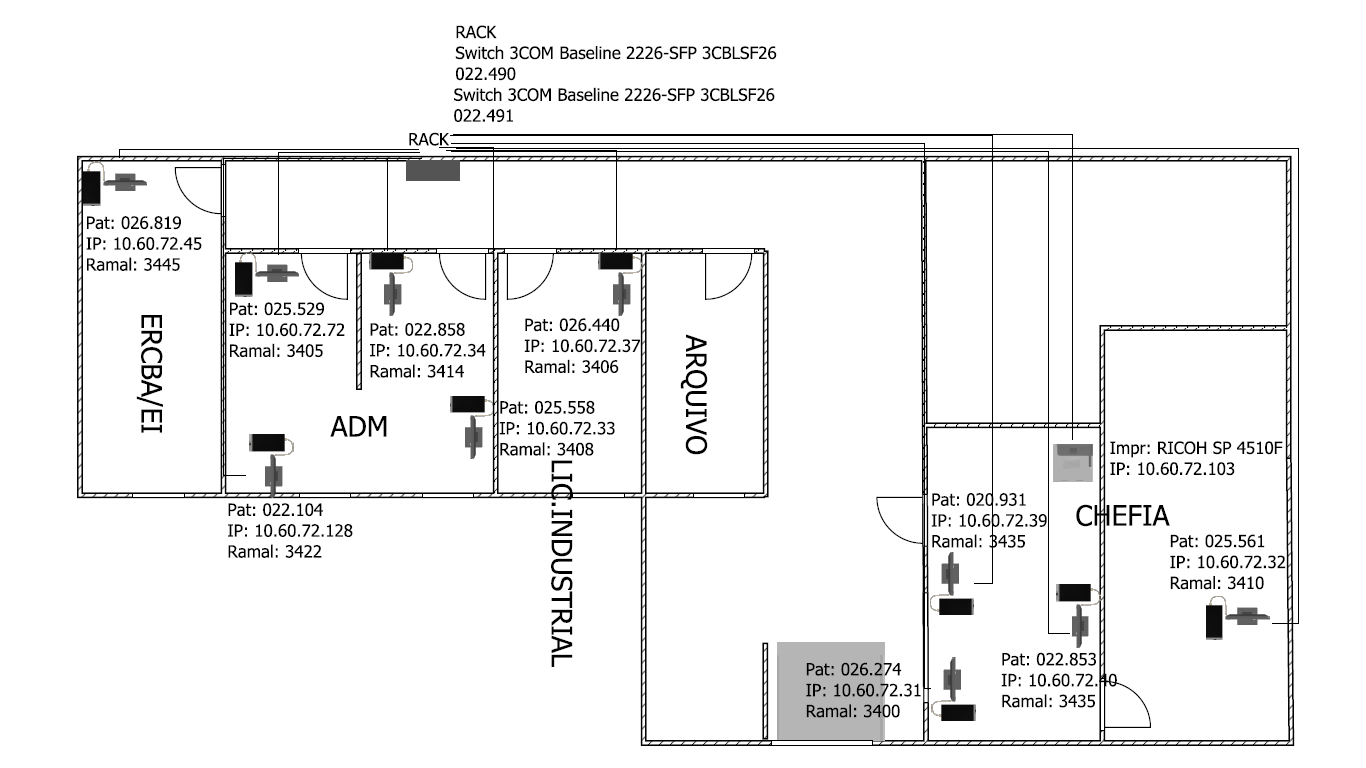
\includegraphics[width=\textwidth]{figura5.png}
	\caption[Trabalho - Térreo]{Estado Atual - Posições das Áreas de Trabalho - Térreo}
	\label{figura5}
\end{figure}
\fi
%==============================A3 INICIO===========================
\clearpage 
\thispagestyle{plain}
\KOMAoptions{paper=a3, paper=landscape, DIV=20}
\recalctypearea
\begin{figure}
	\noindent\makebox[\textwidth][c]{
		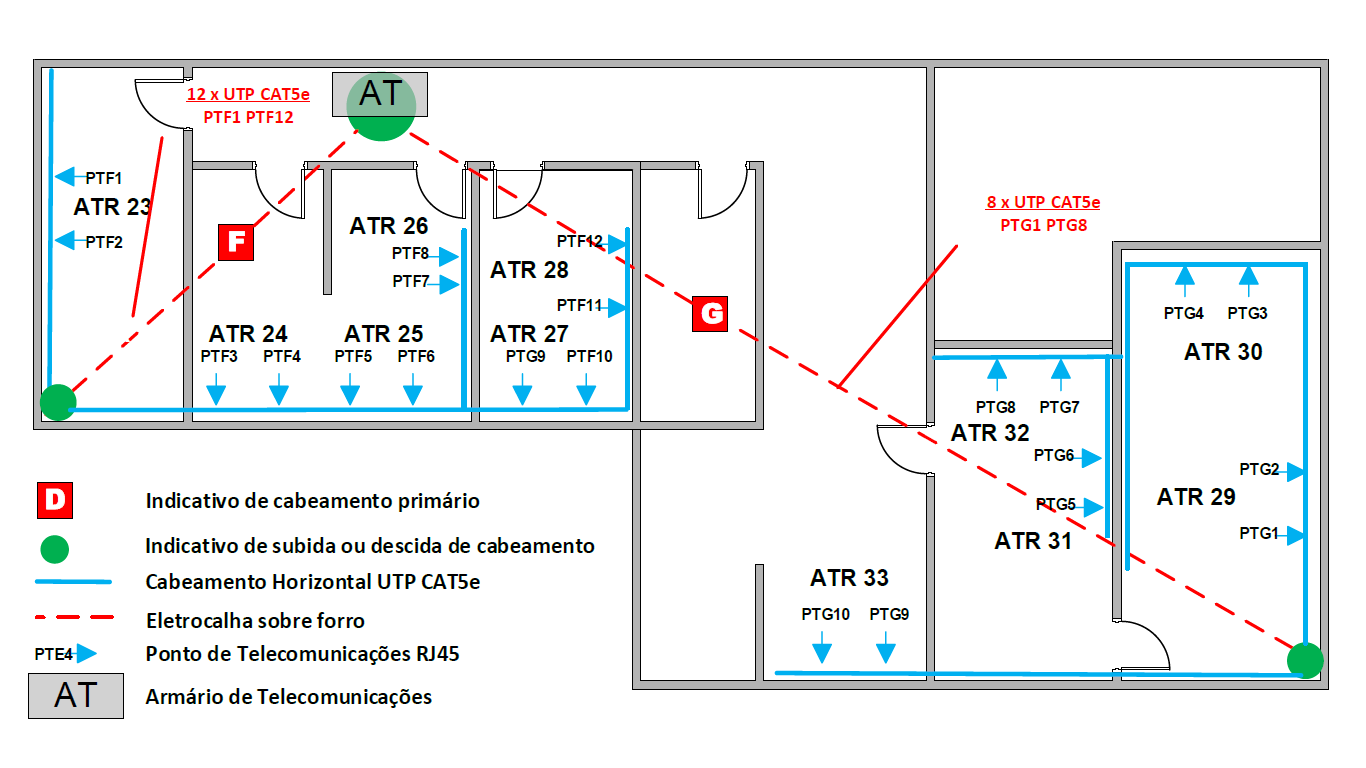
\includegraphics[width=\textwidth]{figura6}
	}
	\caption[Estado Atual - Distribuição Cabeamento Horizontal/Backbone – 1º andar]{Estado Atual - Distribuição Cabeamento Horizontal/Backbone – 1º andar}
		\label{figura6}
\end{figure}

%REVERTER

\clearpage
\KOMAoptions{paper=a4, paper=portrait, DIV=15}
\recalctypearea
%==============================A3 FIM===========================
\iffalse
\begin{figure}[h!]
	\centering
	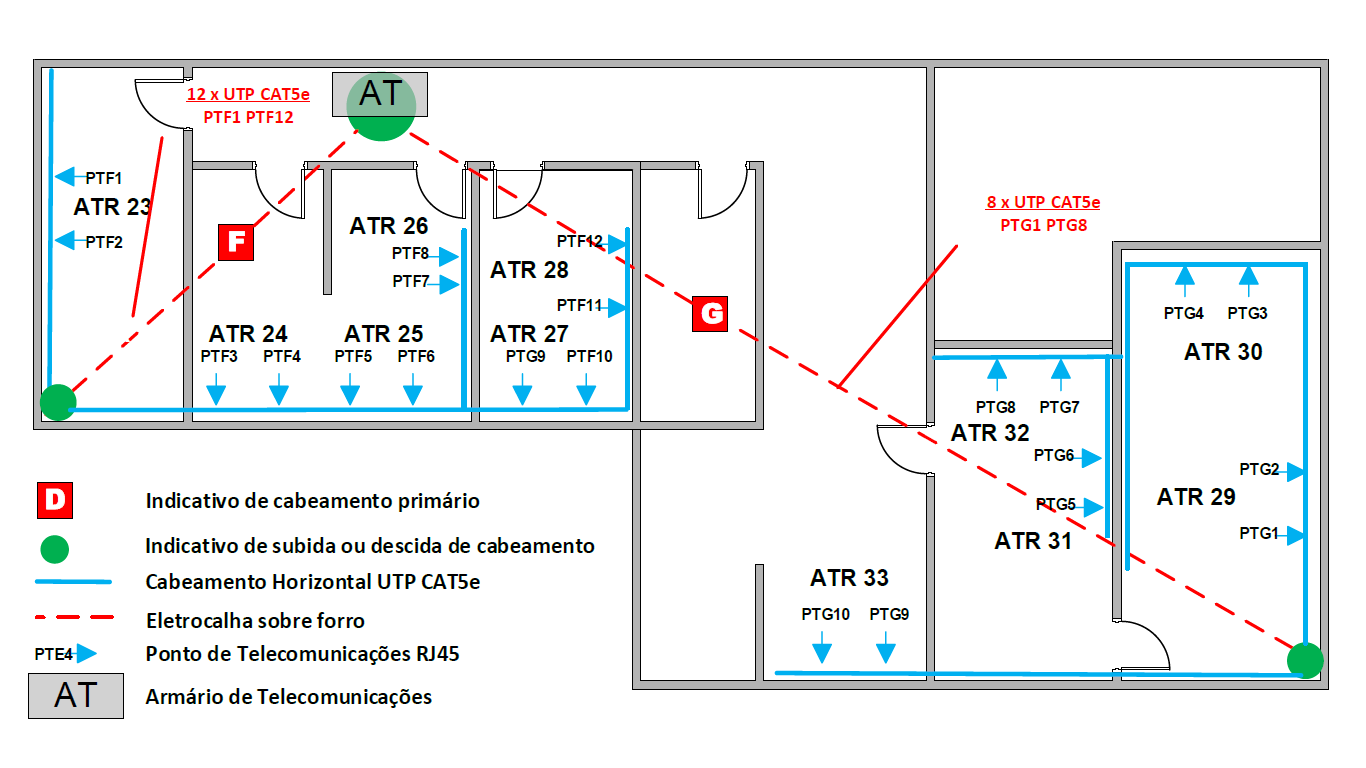
\includegraphics[width=\textwidth]{figura6.png}
	\caption[Estado Atual - Distribuição Cabeamento Horizontal/Backbone – 1º andar]{Estado Atual - Distribuição Cabeamento Horizontal/Backbone – 1º andar}
	\label{figura6}
\end{figure}
\fi
\subsection{Topologia}
%Proposta futura, proposta após implantação.
%Deve conter o diagrama da rede. Atente-se a redundância  e ligações truncadas.
%Deve explicar todos termos e componentes utilizados nestas plantas. Por exemplo: entrance facility, work area, horizontal cabling, etc..

%Todos os elementos das figuras devem ser explicados. 
%Crie esboço da configuração dos racks e brackets. Explique cada um dos componentes. Você pode criar uma tabela contendo figuras dentro, ou criar uma tabela e incluí-la como imagem. Por exemplo, verifique a tabela \ref{tab1}.
No diagrama abaixo é possível contemplar de maneira visual como se organizam e interagem todos os elementos que compõem a estrutura do projeto.\par
Em primeiro lugar temos o DGT (Distribuidor Geral de Telecomunicações) o qual também podemos chamar de \textit{entrance facility}. É no nosso DGT que entram os serviços externos de telecomunicações que serão distribuídos para toda a edificação por meio do nosso sistema de cabeamento estruturado.\par
Advindos do DGT (baseado no diagrama descrito por COMER \cite{COMER}), tais links entram em nossa SEQ (Sala de Equipamentos), onde alimentarão nossos ativos de rede como o roteador e os \textit{switches} e a conexão será distribuída para todas as áreas de trabalho por meio dos cabeamentos principais, representados no diagrama pelas letras de A a G, assim sendo, somando sete troncos principais de cabeamento principal. De cada um desses troncos principais derivam as áreas de trabalho, nomeadas de ATR1 até ATR33, sendo que de cada uma delas saem os pontos de rede que alimentarão as MUTO’s, tomadas multiusuários.

\begin{table}[h!]
	\onehalfspacing
	\caption{Tabela Explicativa dos Elementos Constituintes da Rede}
	\vspace{0.5cm}
	\centering
	\renewcommand{\arraystretch}{1.4}
	\label{tab3}
	\resizebox{\textwidth}{!}{%
	\begin{tabular}{|l|l|}
		\hline
		\multicolumn{1}{|c|}{\textbf{Elemento}} & \multicolumn{1}{c|}{{\color[HTML]{000000} \textbf{Função}}}                                                                                                                                                                                                        \\ \hline
		DGT                                     & {\color[HTML]{000000} Distribuidor Geral de Telecomunicações}                                                                                                                                                                                                      \\ \hline
		{\color[HTML]{000000} SEQ}              & {\color[HTML]{000000} Sala de Equipamentos}                                                                                                                                                                                                                        \\ \hline
		A, B, C, D, E, F, G                     & {\color[HTML]{000000} Cabeamento Horizontal Sobre Forro}                                                                                                                                                                                                           \\ \hline
		ART                                     & {\color[HTML]{000000} \begin{tabular}[c]{@{}l@{}}Cabeamento Horizontal Baixo, encaminhado via calhas de rodapé, os \\ quais atendem cada uma das áreas de trabalho. Sua identificação é composta \\ por: ART+”Nº da área de trabalho correspondente”\end{tabular}} \\ \hline
		PTXN                                    & {\color[HTML]{000000} \begin{tabular}[c]{@{}l@{}}Pontos de Rede RJ45 com sua devida identificação, composta pelo padrão: \\ PT+”Letra do Cabeamento Horizontal Sobre Forro”+”Nº do Ponto”\end{tabular}}                                                            \\ \hline
	\end{tabular}
}
\end{table}

%==============================A3 INICIO===========================
\clearpage 
\thispagestyle{plain}
\KOMAoptions{paper=a3, paper=landscape, DIV=20}
\recalctypearea
\begin{figure}
	\noindent\makebox[\textwidth][c]{
		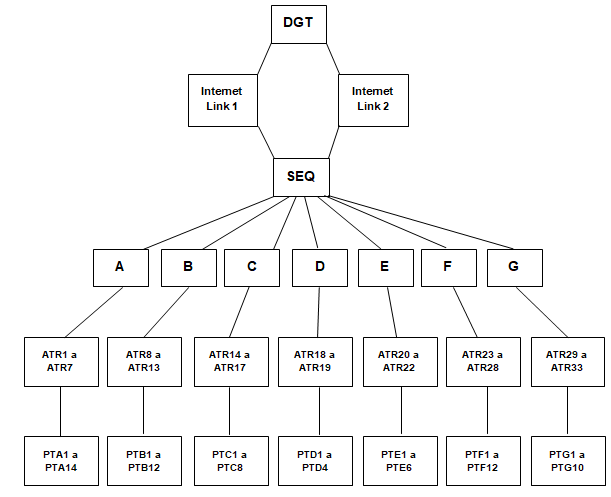
\includegraphics[width=\textwidth]{figura7}
	}
	\caption[Diagrama da Topologia da Rede]{Diagrama da Topologia da Rede}
	\label{figura7}
\end{figure}

%REVERTER

\clearpage
\KOMAoptions{paper=a4, paper=portrait, DIV=15}
\recalctypearea
%==============================A3 FIM===========================
%\iffalse
%\begin{figure}[h!]
%	\centering
%	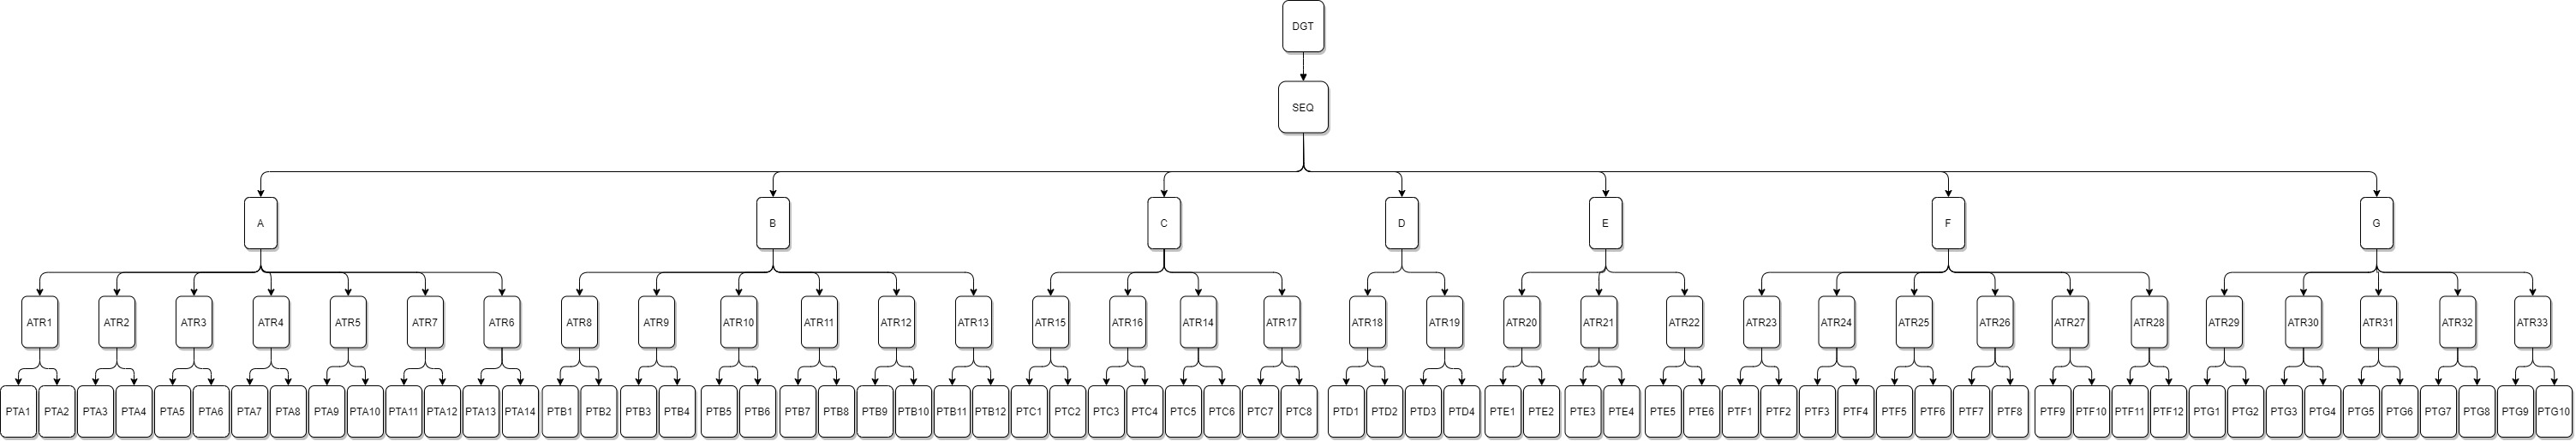
\includegraphics[width=\textwidth]{figura7.jpg}
%	\caption[Diagrama da Topologia da Rede]{Diagrama da Topologia da Rede}
%	\label{figura7}
%\end{figure}
%\fi
\clearpage
\subsection{Encaminhamento}
%Eletrodutos, calhas, e qualquer material em que os cabos serão alojados/alocados.
\begin{itemize}
\item Condulete E de 1”: condulete de alumínio, sem rosca, para eletroduto de 1“:
\begin{figure}[h!]
	\centering
	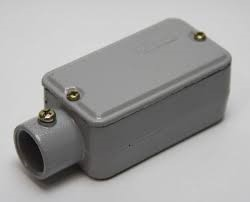
\includegraphics[width=0.2\textwidth]{figura16.jpg}
	\label{figura16}
	\caption{Condulete E de 1"}
\end{figure}
\item Condulete C de 1”: condulete de alumínio, sem tampa, sem rosca, para eletroduto de 1”:
\begin{figure}[h!]
	\centering
	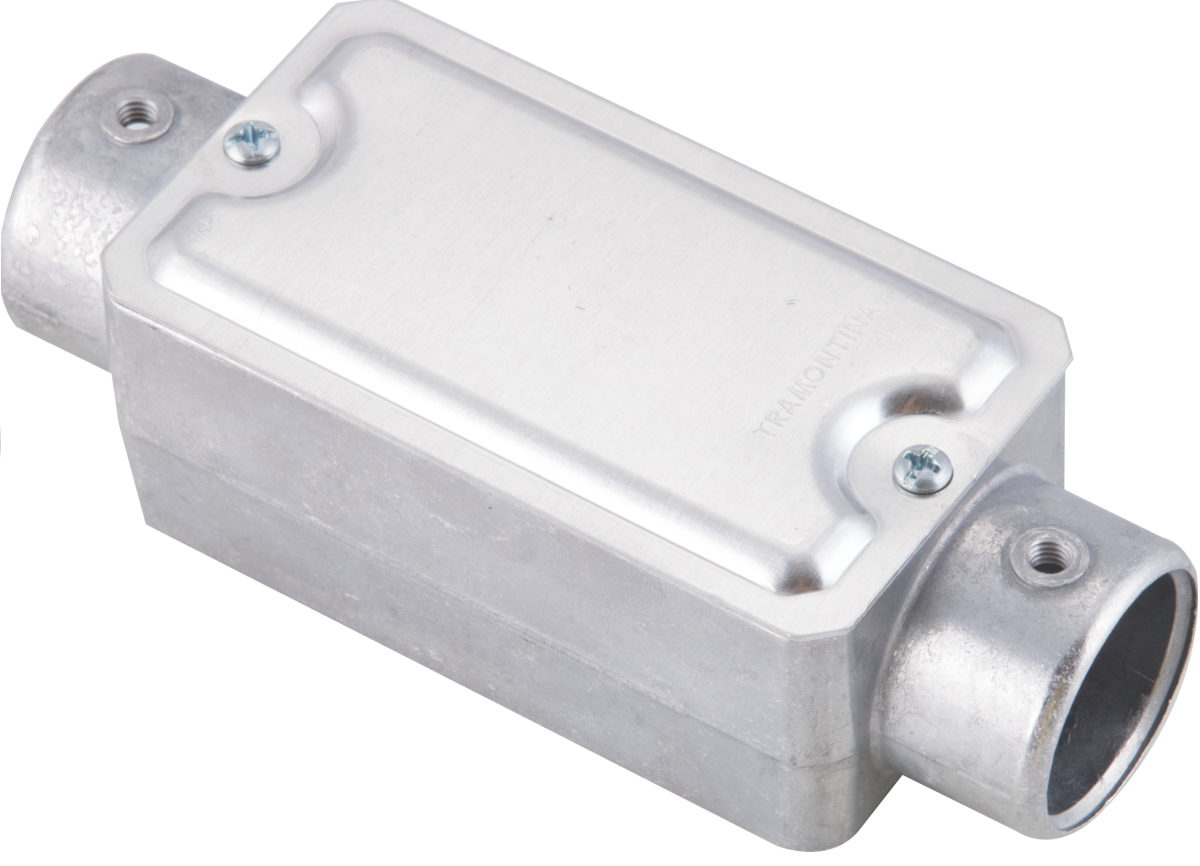
\includegraphics[width=0.2\textwidth]{figura15.png}
	\label{figura15}
	\caption{Condulete C de 1"}
\end{figure}
\item Condulete para eletroduto múltiplo 1’’ em aço galvanizado curva, com diâmetro de 1”:
\begin{figure}[h!]
	\centering
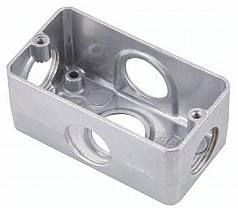
\includegraphics[width=0.2\textwidth]{figura17.jpeg}
	\label{figura17}
	\caption{Condulete para eletroduto múltiplo 1’’}
\end{figure}
\item Curva para eletroduto de 1” em aço galvanizado curva para eletroduto em aço galvanizado, com diâmetro de 1” e parede com espessura mínima de 1,0mm:
\begin{figure}[h!]
	\centering
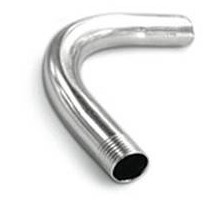
\includegraphics[width=0.2\textwidth]{figura18.jpg}
	\label{figura18}
	\caption{Curva para eletroduto de 1” em aço galvanizado}
\end{figure}
\newpage
\item Eletroduto de 1” em aço galvanizado eletroduto em aço galvanizado, com diâmetro de 1”, parede com espessura mínima de 1,0mm e comprimento da barra de 3m:
\begin{figure}[h!]
	\centering
	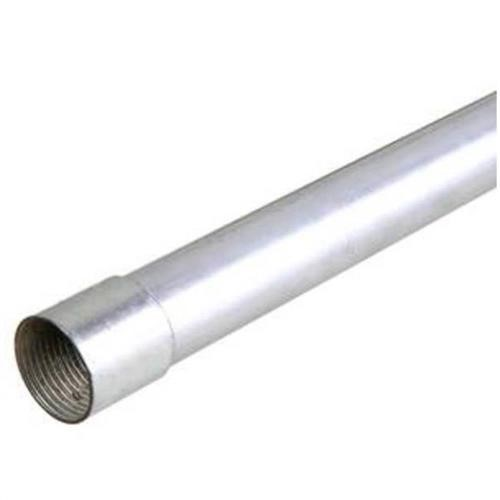
\includegraphics[width=0.2\textwidth]{figura19.jpg}
	\label{figura19}
	\caption{Eletroduto de 1” em aço galvanizado eletroduto em aço galvanizado}
\end{figure}
\item Luva para eletroduto de 1” em aço galvanizado luva para eletroduto em aço galvanizado, com diâmetro de 1”:
\begin{figure}[h!]
	\centering
	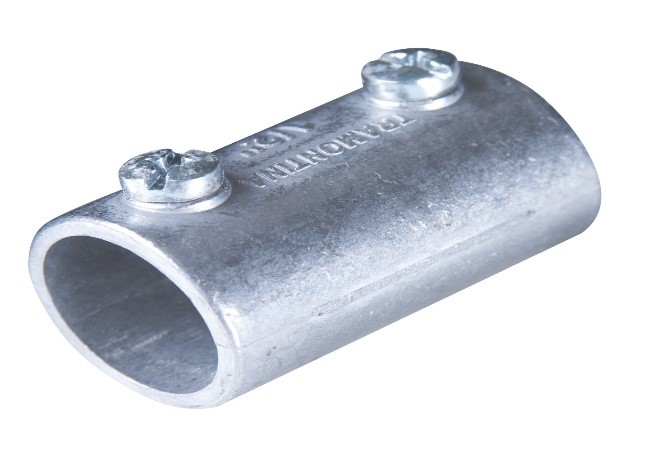
\includegraphics[width=0.2\textwidth]{figura20.jpg}
	\label{figura20}
	\caption{Luva para eletroduto de 1” em aço galvanizado}
\end{figure}
\item Abraçadeira galvanizada "D" para eletroduto 3/4":
\begin{figure}[h!]
	\centering
	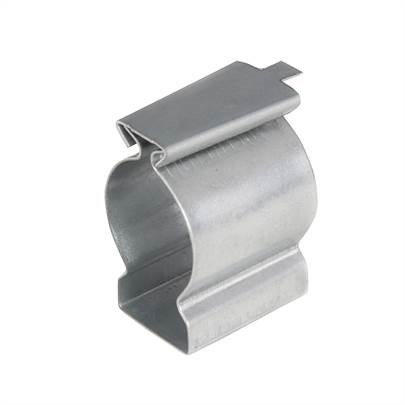
\includegraphics[width=0.2\textwidth]{figura21.jpg}
	\label{figura21}
	\caption{Abraçadeira galvanizada "D" para eletroduto 3/4"}
\end{figure}
\end{itemize}
\newpage
\subsection{Memorial descritivo}
\begin{table}[h!]
	\onehalfspacing
	\caption{Memorial descritivo}
	\vspace{0.5cm}
	\centering
	\renewcommand{\arraystretch}{1.4}
	\label{tab4}
	\resizebox{\textwidth}{!}{%
	\begin{tabular}{|l|l|}
		\hline
		\multicolumn{1}{|c|}{\textbf{Componente}}                           & \multicolumn{1}{c|}{\textbf{Quantidade}} \\ \hline
		Patch Panel Cat5e 24 Portas SohoPlus - 1666                         & 03 und                                   \\ \hline
		NoBreak 1500VA Net4+ Monovolt 115v 27297 - 6150                     & 02 und                                   \\ \hline
		Conjunto Montado Aria 4x2 1 Tomada De Rede/internet Rj45 Tramontina & 66 und                                   \\ \hline
		Régua de Tomada Novo Padrăo de 10A com 12 Tomadas - 1487            & 02 und                                   \\ \hline
		Patch Cord Cat5e Importado Azul                                     & 140 und                                  \\ \hline
		Mini Rack de Parede 16U por 570mm Preto                             & 01 und                                   \\ \hline
		Mini Rack de Parede 7U                                              & 01 und                                   \\ \hline
		Cabo de Rede Cat5e SohoPlus Azul                                    & 1350 mts                                 \\ \hline
		Condulete C de 1"                                                   & 47 und                                   \\ \hline
		Condulete E de 1"                                                   & 08 und                                   \\ \hline
		Condulete para eletroduto múltiplo 1"                               & 11 und                                   \\ \hline
		Curva para eletroduto de 1"                                         & 14 und                                   \\ \hline
		Eletroduto de 1" em aço galvanizado 3 metros                        & 45 und                                   \\ \hline
		Luva para eletroduto de 1"                                          & 15 und                                   \\ \hline
		Abraçadeira galvanizada "D"                                         & 130 und                                  \\ \hline
		\end{tabular}
	}
\end{table}
%Relacione todos os equipamentos passivos que serão utilizados, tipo, fabricante, quantidade.
\subsection{Identificação dos cabos}
%Explique como os cabos serão identificados em seu projeto. Coloque uma relação dos cabos instalados e identificados.
Seguindo a orientação da norma ABNT NBR14565, bem como o que nos diz \cite[Marin]{Marin}, sobre a identificação de cabos, de tal maneira desenvolvemos um padrão para as etiquetas capaz de identificar e rastrear cada cabo, relacionando-o com sua localização de acordo com a ATR (Área de Trabalho) a qual pertence, bem como com o cabeamento primário de onde se originou.
Como exemplo temos a etiqueta de identificação com o código ATR25-PTF6, onde: 
\begin{itemize}
\item ATR25: corresponde a área de trabalho de número 25;
\item PTF6: corresponde ao ponto de rede 6, proveniente do cabeamento primário “F”;
\end{itemize}
\begin{figure}[h!]
	\centering
	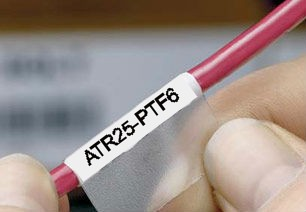
\includegraphics[width=0.4\textwidth, height=1\textheight, keepaspectratio=true]{figura8.jpg}
	\caption[Etiqueta de identificação dos cabos]{Etiqueta de identificação dos cabos}
	\label{figura8}
\end{figure}

\section{Implantação}
%Estabeleça um cronograma de implantação:
%Remoção de equipamentos existentes (destino para descarte), instalação dos condutores, instalação dos cabos, 
%identificação dos cabos, montagem dos racks, certificação, etc... Crie atividades e estabeleça o tempo de execução. Se for um projeto real, indique também quais os responsáveis pela execução do projeto e de cada uma das etapas.

%Defina marcas (e padrões) e fornecedores se for o caso. Atenção a contratados e subcontratados para a realização das atividades. Estabeleça a responsabilidade de execução da atividade e também da validação dela.

%Utilize algum software para gerear o cronograma. Excel,etc. O fundamental é dividir em etapas, descrever e estimar o tempo de cada uma delas.

%Segue uma relação de ferramentas:
%http://asana.com/, \\
%https://trello.com/, \\
%http://www.ganttproject.biz/, \\
%http://www.orangescrum.org/.
Abaixo segue o cronograma de implantação da rede projetada para o Instituto Ambiental do Paraná, nele é possível observar todas as etapas rastreadas, desde o levantamento de requisitos até a entrega do serviço e da documentação final produzida durante a execução de todo o projeto.
Para desenvolvimento desse cronograma e seu respectivo gráfico de Gantt, foi utilizada a ferramenta online: \href{https://app.instagantt.com/}{https://app.instagantt.com/} 

\clearpage 
\thispagestyle{plain}
\KOMAoptions{paper=a3, paper=landscape, DIV=20}
\recalctypearea
\begin{figure}
	\noindent\makebox[\textwidth][c]{
		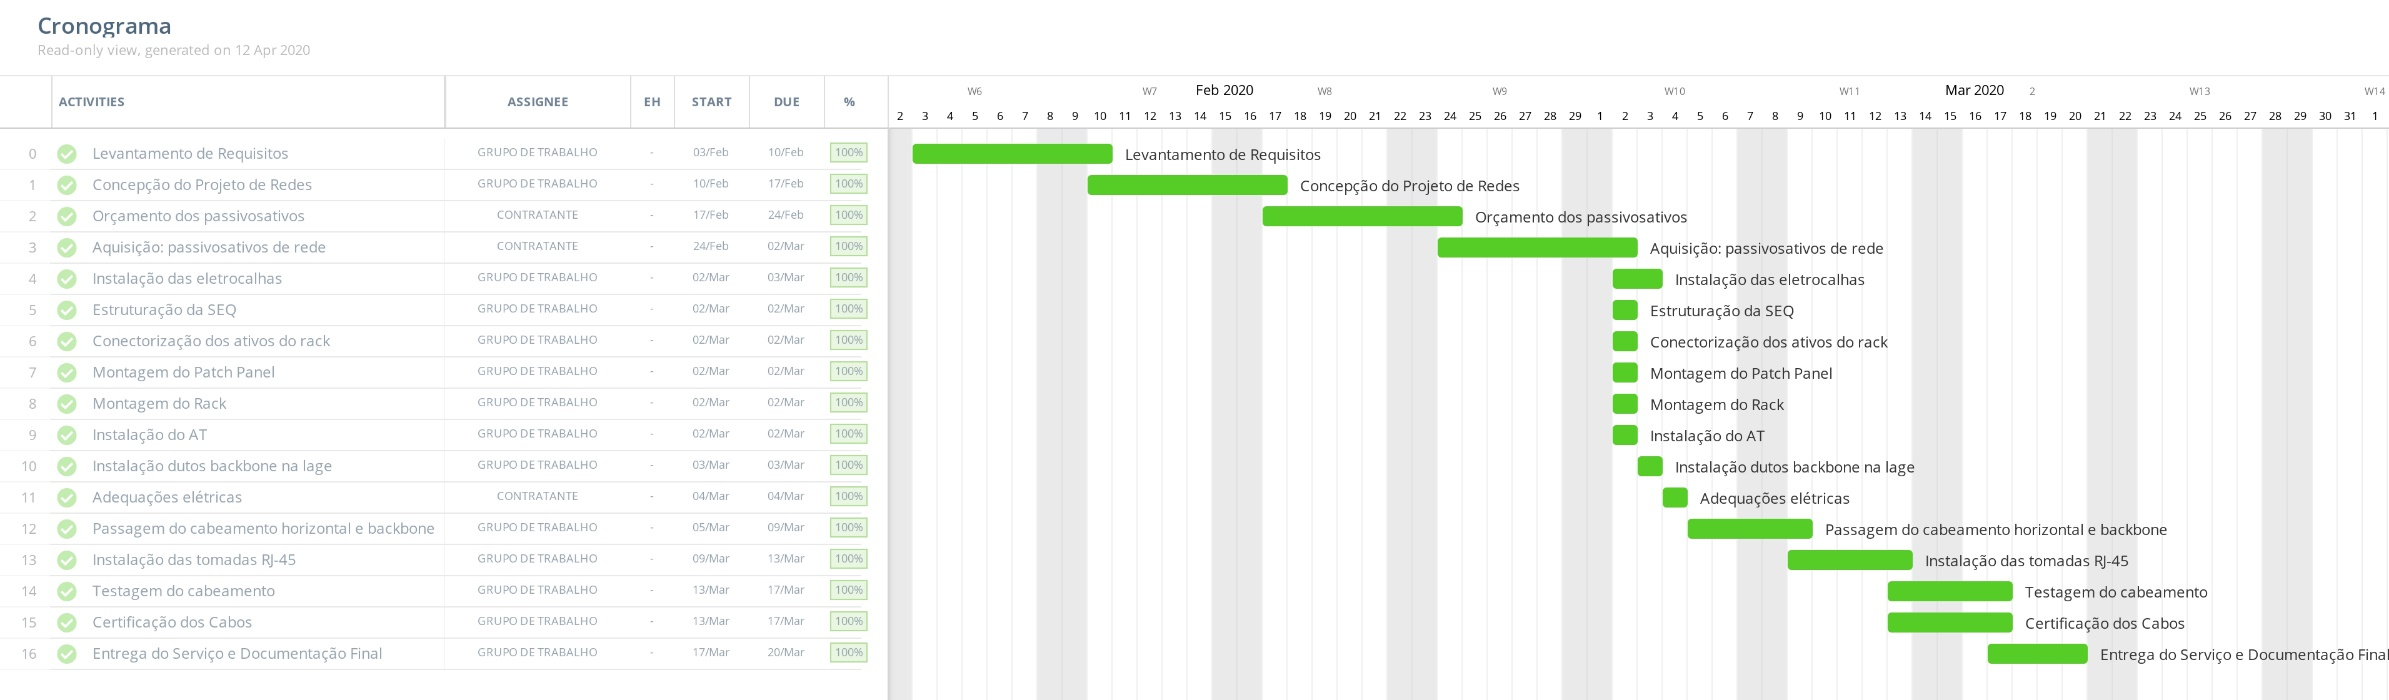
\includegraphics[width=\textwidth]{figura9}
	}
	\caption[Cronograma de atividades e Gráfico de Gantt]{Cronograma de atividades e Gráfico de Gantt}
	\label{figura9}
\end{figure}

%REVERTER

\clearpage
\KOMAoptions{paper=a4, paper=portrait, DIV=15}
\recalctypearea
%==============================A3 FIM===========================


\section{Plano de certificação}
A certificação da planta se dará após completo o processo de implantação e antes do início de operação da rede. Toda a estrutura de rede passará pelo processo de certificação.\\
Será agendada uma data e hora com o IAP-PR, para que também possam acompanhar a atividade.\\
No processo serão realizados os seguintes testes:
\begin{itemize}
\vspace{5mm}
\item Wiremap - Teste que verifica a continuidade dos fios;
\item WireLenght - Teste que verifica o comprimento dos cabos;
\item Resistance Test - Teste que verifica a resistência do circuito em cada fio;
\item NEXT/FEXT - Teste que identifica possíveis falhas nos conectores e ruídos gerados por dispositivos externos;
\item Atenuação - Teste que identifica falha de atenuação no cabo;
\item Perda de Retorno - Teste que mede a reflexão no cabo;
\item Impedância - Teste que calcula a impedância do cabo;
\item Testes Delay e Skew - Teste que mede o tempo que um sinal leva para percorrer o cabo e a diferença entre o maior e menor tempo medidos;
\item Capacitância - Teste que mede a capacitância mútua entre os dois condutores de cada par;
\item ACR e Power Sum ACR - Teste que realiza faz a subtração entre os resultados de atenuação e o teste NEXT, em um par (ACR) ou nos outros três pares do cabo (Sum ACR).
\end{itemize}
\par Conforme citado em sua publicação, TANENBAUM \cite{TANENBAUM}, os testes serão realizados a fim de alcançar a certificação Cat5E.
Caso algum teste não obtenha os resultados esperados, será identificado o cabo ou cabos com problema para que sejam efetuadas as correções necessárias para o alcance da certificação.\par
Após o fim do processo, será entregue um relatório ao IAP-PR contendo todos os resultados obtidos nos testes acima mencionados.

\section{Plano de manutenção}
A instalação possui um ano de garantia contra defeitos em cabeamento e conectores. Não está incluso o serviço de mudança de pontos e certificações de novos pontos. É possível ao IAP, dentro do período de garantia, solicitar até 3 (três) manutenções preventivas, a fim de identificar e prevenir a ocorrência de falhas na rede.\par
Como se trata de órgão público, a posterior contratação de empresa para manutenção, mudança ou criação de novos pontos dependerá de novo processo licitatório

%Revisões periódicas na rede, emissão de certificados para novos pontos.

\subsection{Plano de expansão}
%Existe um plano de expansão? Quantos novos pontos poderão ser acrecidos na rede, antes de migração de equipamentos na camada 2? Se houver expansão, quais equipamentos deverão ser direcionados para as estremidades da rede? 
Não há plano de expansão para a rede, uma vez que a infraestrutura predial não suporta mais estações de trabalho devido a limitações físicas.\par
Porém em caso de necessidade de ampliação, a margem é ínfima pois sobrarão poucos recursos de rede sem utilização. No térreo estão previstos 44 pontos de comunicação RJ45, além do cascateamento entre os dois switches do térreo e o cabeamento vertical para o switch do primeiro andar, totalizando 47 portas em uso. Ainda há a abordagem do provedor de telecomunicações, que caso ocorra em mídia elétrica consumirá a última interface RJ45 disponível dos switches. Caso essa abordagem seja óptica utilizando a interface SFP do equipamento, sobrará uma interface RJ45 no térreo.\par
Já no primeiro andar, estão previstos 22 pontos de comunicação RJ45.  Somados ao cabeamento vertical, utilizarão 23 interfaces elétricas de um total de 24 disponíveis no switch.\par
Portanto tanto no térreo quanto no primeiro andar não há margem para ampliação sem a aquisição de novos materiais, como switches e patch pannels com maior densidade de interfaces, além da criação de novos pontos de telecomunicações e cabeamento.

\section{Risco}
%Enumerar e explicar os riscos do projeto.
O objetivo do projeto de cabeamento estruturado é mitigar todas as etapas e diminuir a probabilidade de riscos inerentes ao projeto. Porém mesmo com todos os cuidados ainda há riscos que devemos considerar, baseado nos critérios descritos por GALLO \cite{GALLO}:
\begin{itemize}
\item Como a compra dos materiais utilizados se dará pela internet e de lojas de outras cidades, há o risco de atraso na entrega ou entrega de material diferente do pedido, o que gerará atraso no cronograma do projeto.

\item Devido ao fato do prédio não ser novo, há a possibilidade de encontrar passagens obstruídas, além de dificuldade na passagem das canaletas.

\item Outra questão de infraestrutura a ser considerada é a rede elétrica existente. Falhas e instabilidades nessa área podem provocar instabilidades na rede de dados em geral.

\item Outro risco que apesar de poder ser minimizado com treinamento e supervisão dos responsáveis pela instalação é a falha humana durante a execução das atividades. Estas possíveis falhar serão identificadas durante a certificação e poderão ser corrigidas, porém provocarão atraso na entrega da obra. 

\item Por fim nosso cenário atual mostra que ainda existem riscos externos que não são mensuráveis e podem ocorrer sem responsabilidade de nenhum dos entes do projeto. Como exemplo podemos citar a pandemia do novo Coronavírus que afetaria de sobremaneira o andamento do projeto.
\end{itemize}

\section{Orçamento}
%Crie uma relação de orçamentos baseado na seções anteriores.
Com base nos itens descritos, abaixo a tabela com o orçamento de cada componente:
\begin{table}[h!]
	\onehalfspacing
	\caption{Orçamento}
	\vspace{0.5cm}
	\centering
	\renewcommand{\arraystretch}{1.4}
	\label{tab5}
	\resizebox{\textwidth}{!}{%
	\begin{tabular}{lll|l|}
		\hline
		\multicolumn{1}{|c|}{\textbf{Componente}}                                                 & \multicolumn{1}{c|}{\textbf{Quantidade}} & \multicolumn{1}{c|}{\textbf{Custo Unitário}} & \multicolumn{1}{c|}{\textbf{Custo Total}} \\ \hline
		\multicolumn{1}{|l|}{Switch 24 Portas Fast Ethernet Intelbras SF 2400 QR+}                & \multicolumn{1}{l|}{03 und}              & R\$ 511,90                                   & R\$ 1.535,70                              \\ \hline
		\multicolumn{1}{|l|}{Patch Panel Cat5e 24 Portas SohoPlus - 1666}                         & \multicolumn{1}{l|}{03 und}              & R\$ 155,00                                   & R\$ 465,00                                \\ \hline
		\multicolumn{1}{|l|}{NoBreak 1500VA Net4+ Monovolt 115v 27297 - 6150}                     & \multicolumn{1}{l|}{02 und}              & R\$ 828,45                                   & R\$ 1.656,90                              \\ \hline
		\multicolumn{1}{|l|}{Conjunto Montado Aria 4x2 1 Tomada De Rede/internet Rj45 Tramontina} & \multicolumn{1}{l|}{66 und}              & R\$ 13,10                                    & R\$ 864,60                                \\ \hline
		\multicolumn{1}{|l|}{Régua de Tomada Novo Padrăo de 10A com 12 Tomadas - 1487}            & \multicolumn{1}{l|}{02 und}              & R\$ 59,00                                    & R\$ 118,00                                \\ \hline
		\multicolumn{1}{|l|}{Patch Cord Cat5e Importado Azul}                                     & \multicolumn{1}{l|}{140 und}             & R\$ 5,50                                     & R\$ 770,00                                \\ \hline
		\multicolumn{1}{|l|}{Mini Rack de Parede 16U por 570mm Preto}                             & \multicolumn{1}{l|}{01 und}              & R\$ 470,00                                   & R\$ 470,00                                \\ \hline
		\multicolumn{1}{|l|}{Mini Rack de Parede 7U}                                              & \multicolumn{1}{l|}{01 und}              & R\$ 289,00                                   & R\$ 289,00                                \\ \hline
		\multicolumn{1}{|l|}{Cabo de Rede Cat5e SohoPlus Azul}                                    & \multicolumn{1}{l|}{1350 mts}            & R\$ 1,20                                     & R\$ 1.620,00                              \\ \hline
		\multicolumn{1}{|l|}{Condulete C de 1"}                                                   & \multicolumn{1}{l|}{47 und}              & R\$ 8,50                                     & R\$ 399,50                                \\ \hline
		\multicolumn{1}{|l|}{Condulete E de 1"}                                                   & \multicolumn{1}{l|}{08 und}              & R\$ 7,49                                     & R\$ 59,92                                 \\ \hline
		\multicolumn{1}{|l|}{Condulete para Eletroduto múltiplo 1"}                               & \multicolumn{1}{l|}{11 und}              & R\$ 5,50                                     & R\$ 60,50                                 \\ \hline
		\multicolumn{1}{|l|}{Curva para Eletroduto de 1"}                                         & \multicolumn{1}{l|}{14 und}              & R\$ 5,00                                     & R\$ 70,00                                 \\ \hline
		\multicolumn{1}{|l|}{Eletroduto de 1" em Aço}                                             & \multicolumn{1}{l|}{45 und}              & R\$ 14,50                                    & R\$ 652,50                                \\ \hline
		\multicolumn{1}{|l|}{Luva para Eletroduto de 1"}                                          & \multicolumn{1}{l|}{15 und}              & R\$ 1,50                                     & R\$ 22,50                                 \\ \hline
		\multicolumn{1}{|l|}{Abraçadeira galvanizada "D"}                                         & \multicolumn{1}{l|}{130 und}             & R\$ 3,50                                     & R\$ 455,00                                \\ \hline
		\multicolumn{1}{|l|}{Măo de Obra}                                                         & \multicolumn{1}{l|}{}                    &                                              & R\$ 5.000,00                              \\ \hline
		&                                          &                                              & \textbf{Total: 14.509,12}                          \\ \cline{4-4} 
	\end{tabular}
}
\end{table}

\section{Recomendações}
%Observações e recomendações para o cliente.
Visto o agravamento da qualidade do material da infraestrutura encontrado principalmente no ambiente da Fiscalização, segundo TORRES \cite{TORRES}, as intempéries precisam de cuidado, sendo a recomendação que a manutenção cuide do telhado da edificação, evitando infiltrações e demais prejuízos a solidez do material.\par
A rede será entregue totalmente funcional e pronta para uso. Recomendamos ao cliente evitar fazer qualquer alteração sem o devido acompanhamento na rede pois poderá provocar interrupções e falha em suas conexões.\par
Antes de qualquer alteração em sua estrutura predial, deverão ser observados os mapas de encaminhamentos de cabos e conexões, evitando que alguma obra ou manutenção possa provocar danos no cabeamento estruturado.\par
Está previsto no plano de manutenção até três visitas técnicas que poderão ser utilizadas pelo cliente para dirimir dúvidas e procurar orientações sobre o funcionamento da rede.
\clearpage
\section{Referências} %CONFORME ABNT, SÓ SE ESCREVE 'REFERÊNCIAS'

%%Estão faltando os apontamentos de referências. Geralmente insere-se a referência no arquivo \textbf{referencias.bib} e aqui, somente, faz a citação com barra invertida e cite com o comando \verb\'cite'\ e entre as chaves a variável da referência apontada.

%\cite{Marin}	
%Utilize o mendley, o jabref ou diretamente o bibtex para gerenciar suas referências biliográficas. As referências são criadas automaticamente de acordo com o uso no texto.

%Exemplo: Redes de computadores, segundo \cite{t2013} é considerada..... Já \cite{kurose2010} apresenta uma versão...

%Analisando os pressupostos de \cite{ref3} e \cite{ref4} concluimos que....


\renewcommand\refname{} %%Referências bibliográficas}  
\bibliographystyle{ieeetr}
\bibliography{referencias}  

%% ***********************************************************************
%% === remover daqui =====================================================
%% ***********************************************************************

%%\section{Elementos textuais - Alguns exemplos}

%%Esta seção apresenta exemplos de elementos textuais. \textbf{Remova-a da versão final do texto}.


%%\subsection{Colocar elementos em itens}

%%Texto antes da lista

%%\begin{itemize}
%%	\item First item in a list 
%%	\item Second item in a list 
%%	\item Third item in a list
%%\end{itemize}

%%\subsubsection{Uma subseção de terceiro nivel}

%%Exemplo de uma subseção Tabela \ref{tab1}

%%\subsection{Tabelas}

%%Utilize o site http://www.tablesgenerator.com/ para elaborar as tabelas de seu trabalho.
%%Para adicionar uma tabela utilize: a tag input, passando o arquivo da tabela como parametro
%%\begin{table}[h!]
	\onehalfspacing
	\caption{Tabela Explicativa dos Elementos Constituintes da Rede}
	\vspace{0.5cm}
	\centering
	\renewcommand{\arraystretch}{1.4}
	\label{tab3}
	\resizebox{\textwidth}{!}{%
	\begin{tabular}{|l|l|}
		\hline
		\multicolumn{1}{|c|}{\textbf{Elemento}} & \multicolumn{1}{c|}{{\color[HTML]{000000} \textbf{Função}}}                                                                                                                                                                                                        \\ \hline
		DGT                                     & {\color[HTML]{000000} Distribuidor Geral de Telecomunicações}                                                                                                                                                                                                      \\ \hline
		{\color[HTML]{000000} SEQ}              & {\color[HTML]{000000} Sala de Equipamentos}                                                                                                                                                                                                                        \\ \hline
		A, B, C, D, E, F, G                     & {\color[HTML]{000000} Cabeamento Horizontal Sobre Forro}                                                                                                                                                                                                           \\ \hline
		ART                                     & {\color[HTML]{000000} \begin{tabular}[c]{@{}l@{}}Cabeamento Horizontal Baixo, encaminhado via calhas de rodapé, os \\ quais atendem cada uma das áreas de trabalho. Sua identificação é composta \\ por: ART+”Nº da área de trabalho correspondente”\end{tabular}} \\ \hline
		PTXN                                    & {\color[HTML]{000000} \begin{tabular}[c]{@{}l@{}}Pontos de Rede RJ45 com sua devida identificação, composta pelo padrão: \\ PT+”Letra do Cabeamento Horizontal Sobre Forro”+”Nº do Ponto”\end{tabular}}                                                            \\ \hline
	\end{tabular}
}
\end{table}

%%Dentro do arquivo você deve definir o label e pode utilizá-lo para referenciar. Exemplo:
%%Na tab \ref{tab2} temos a relação de ....


%%Você também pode modificar a tabela manualmente, incluindo, por exemplo h! dentro de sua definição. Veja no exemplo tab2.tex

%%\subsection{Figuras}

%%As figuras podem ser no formato PDF, JPG, PNG. Você pode referenciá-las da mesma maneira que tabelas. Exemplo: A figura \ref{fig1} apresenta.....

%%Não se preocupe o local em que a figura será renderizada em seu texto. Preocupe-se em criar referência para ela, ou seja, toda figura e tabela deve conter pelo menos uma referência no texto.

%%\begin{figure}
%%\centering
%%\includegraphics[width=\textwidth]{fig1}
%%\caption{Exemplo de figura com escala horizontal}
%%\label{fig1}
%%\end{figure}


%%\begin{figure}
%%	\centering
%%	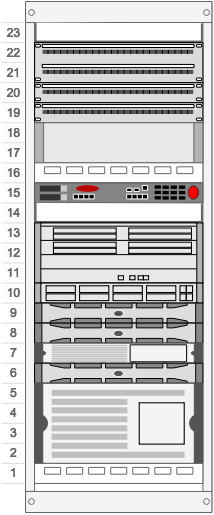
\includegraphics[]{fig2}
%%	\caption{Exemplo de figura sem escala}
%%	\label{fig2}
%%\end{figure}

%%Você pode rotacionar figuras também. Para isso utilize o parâmetro angle=-90. Repare que a escala da figura foi modificada pelo parametro height. Você também pode utilizar scale

%%\begin{figure}
%%	\centering
%%	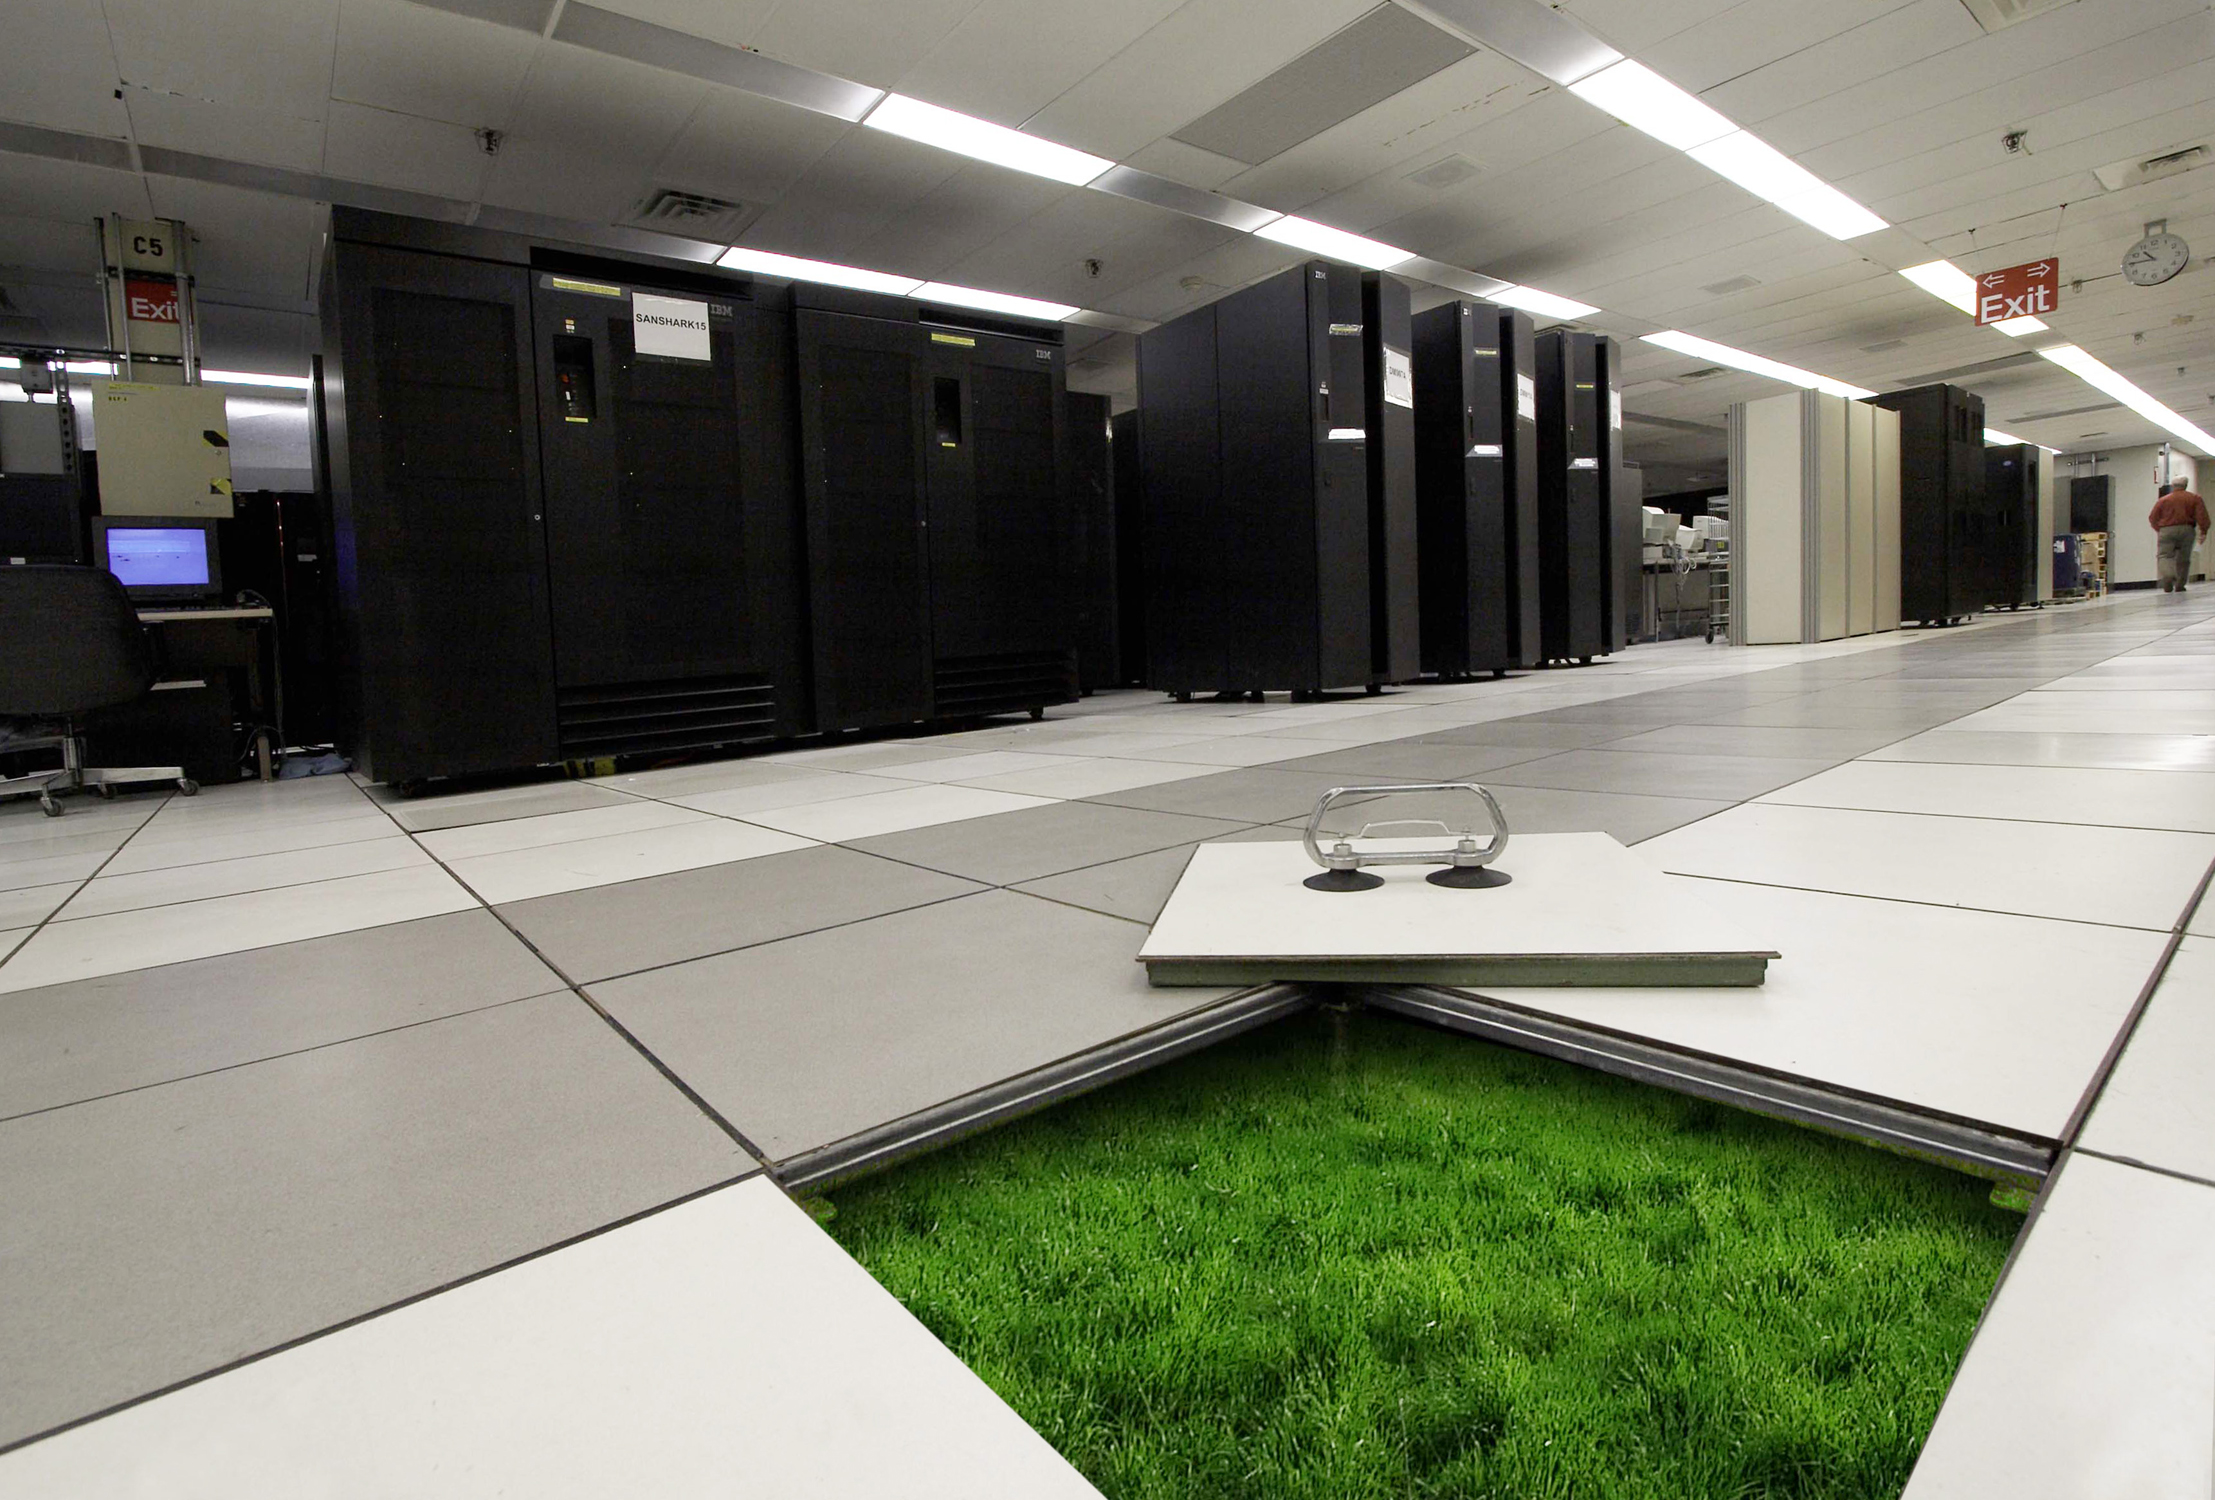
\includegraphics[height=\textwidth,angle=-90]{fig3}
%%	\caption{Exemplo de figura rotacionada}
%%	\label{fig3}
%%\end{figure}

%%Você também pode inserir páginas de outro tamanho em seu texto. Isto irá ajudar a inserir imagens maiores, como as desenvolvidas em CAD. Segue um exemplo na figura \ref{fig4} e figura \ref{fig5}.


%inicio dos comandos para criar uma nova pagina A3
%%\clearpage
%%\KOMAoptions{paper=a3, pagesize}
%%\recalctypearea

%%\begin{figure}
%%	\centering
%%	\makebox[\textwidth][c]{
%%		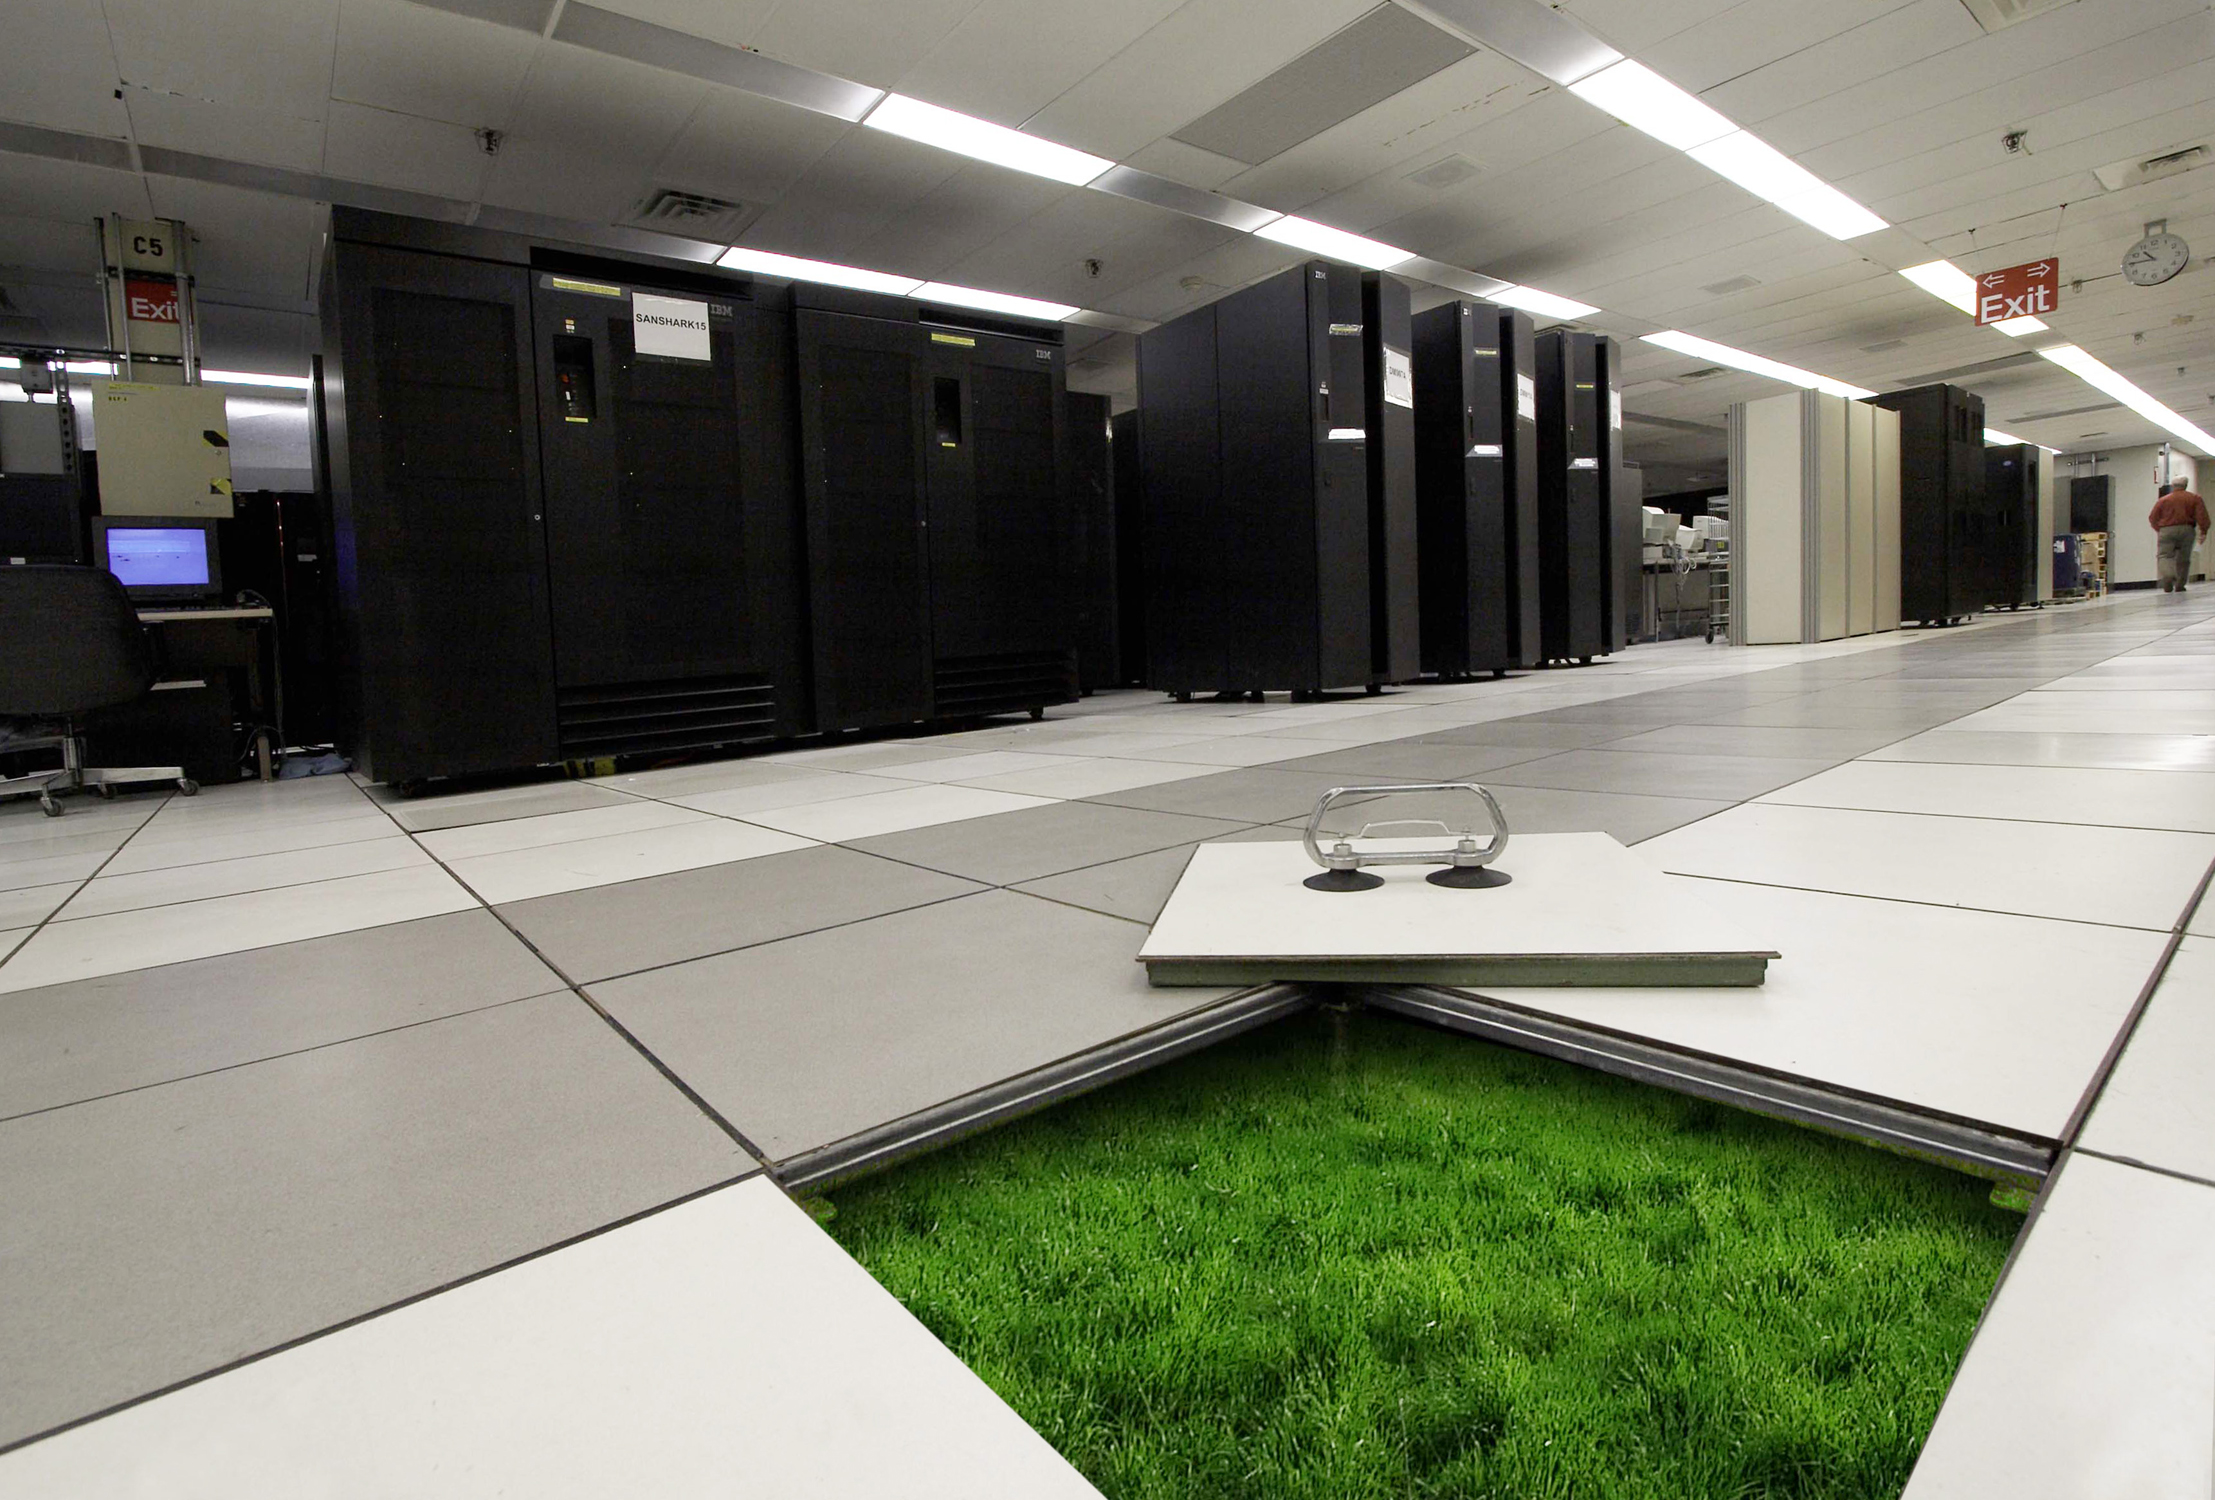
\includegraphics[height=\textheight]{fig3}}
%%	\caption{Exemplo de figura inserida em uma página A3}
%%	\label{fig4}
%%\end{figure}

%Retornar ao formato A4
%%\clearpage
%%\KOMAoptions{paper=a4, pagesize}
%%\recalctypearea
%-- reinicio em A4 


%inicio dos comandos para criar uma nova pagina A3 horizontal
%%\clearpage
%%\KOMAoptions{paper=a3, paper=landscape, DIV=20}
%%\recalctypearea

	
%%\begin{figure}
%%	\centering
%%	\noindent\makebox[\textwidth][c]{
%%		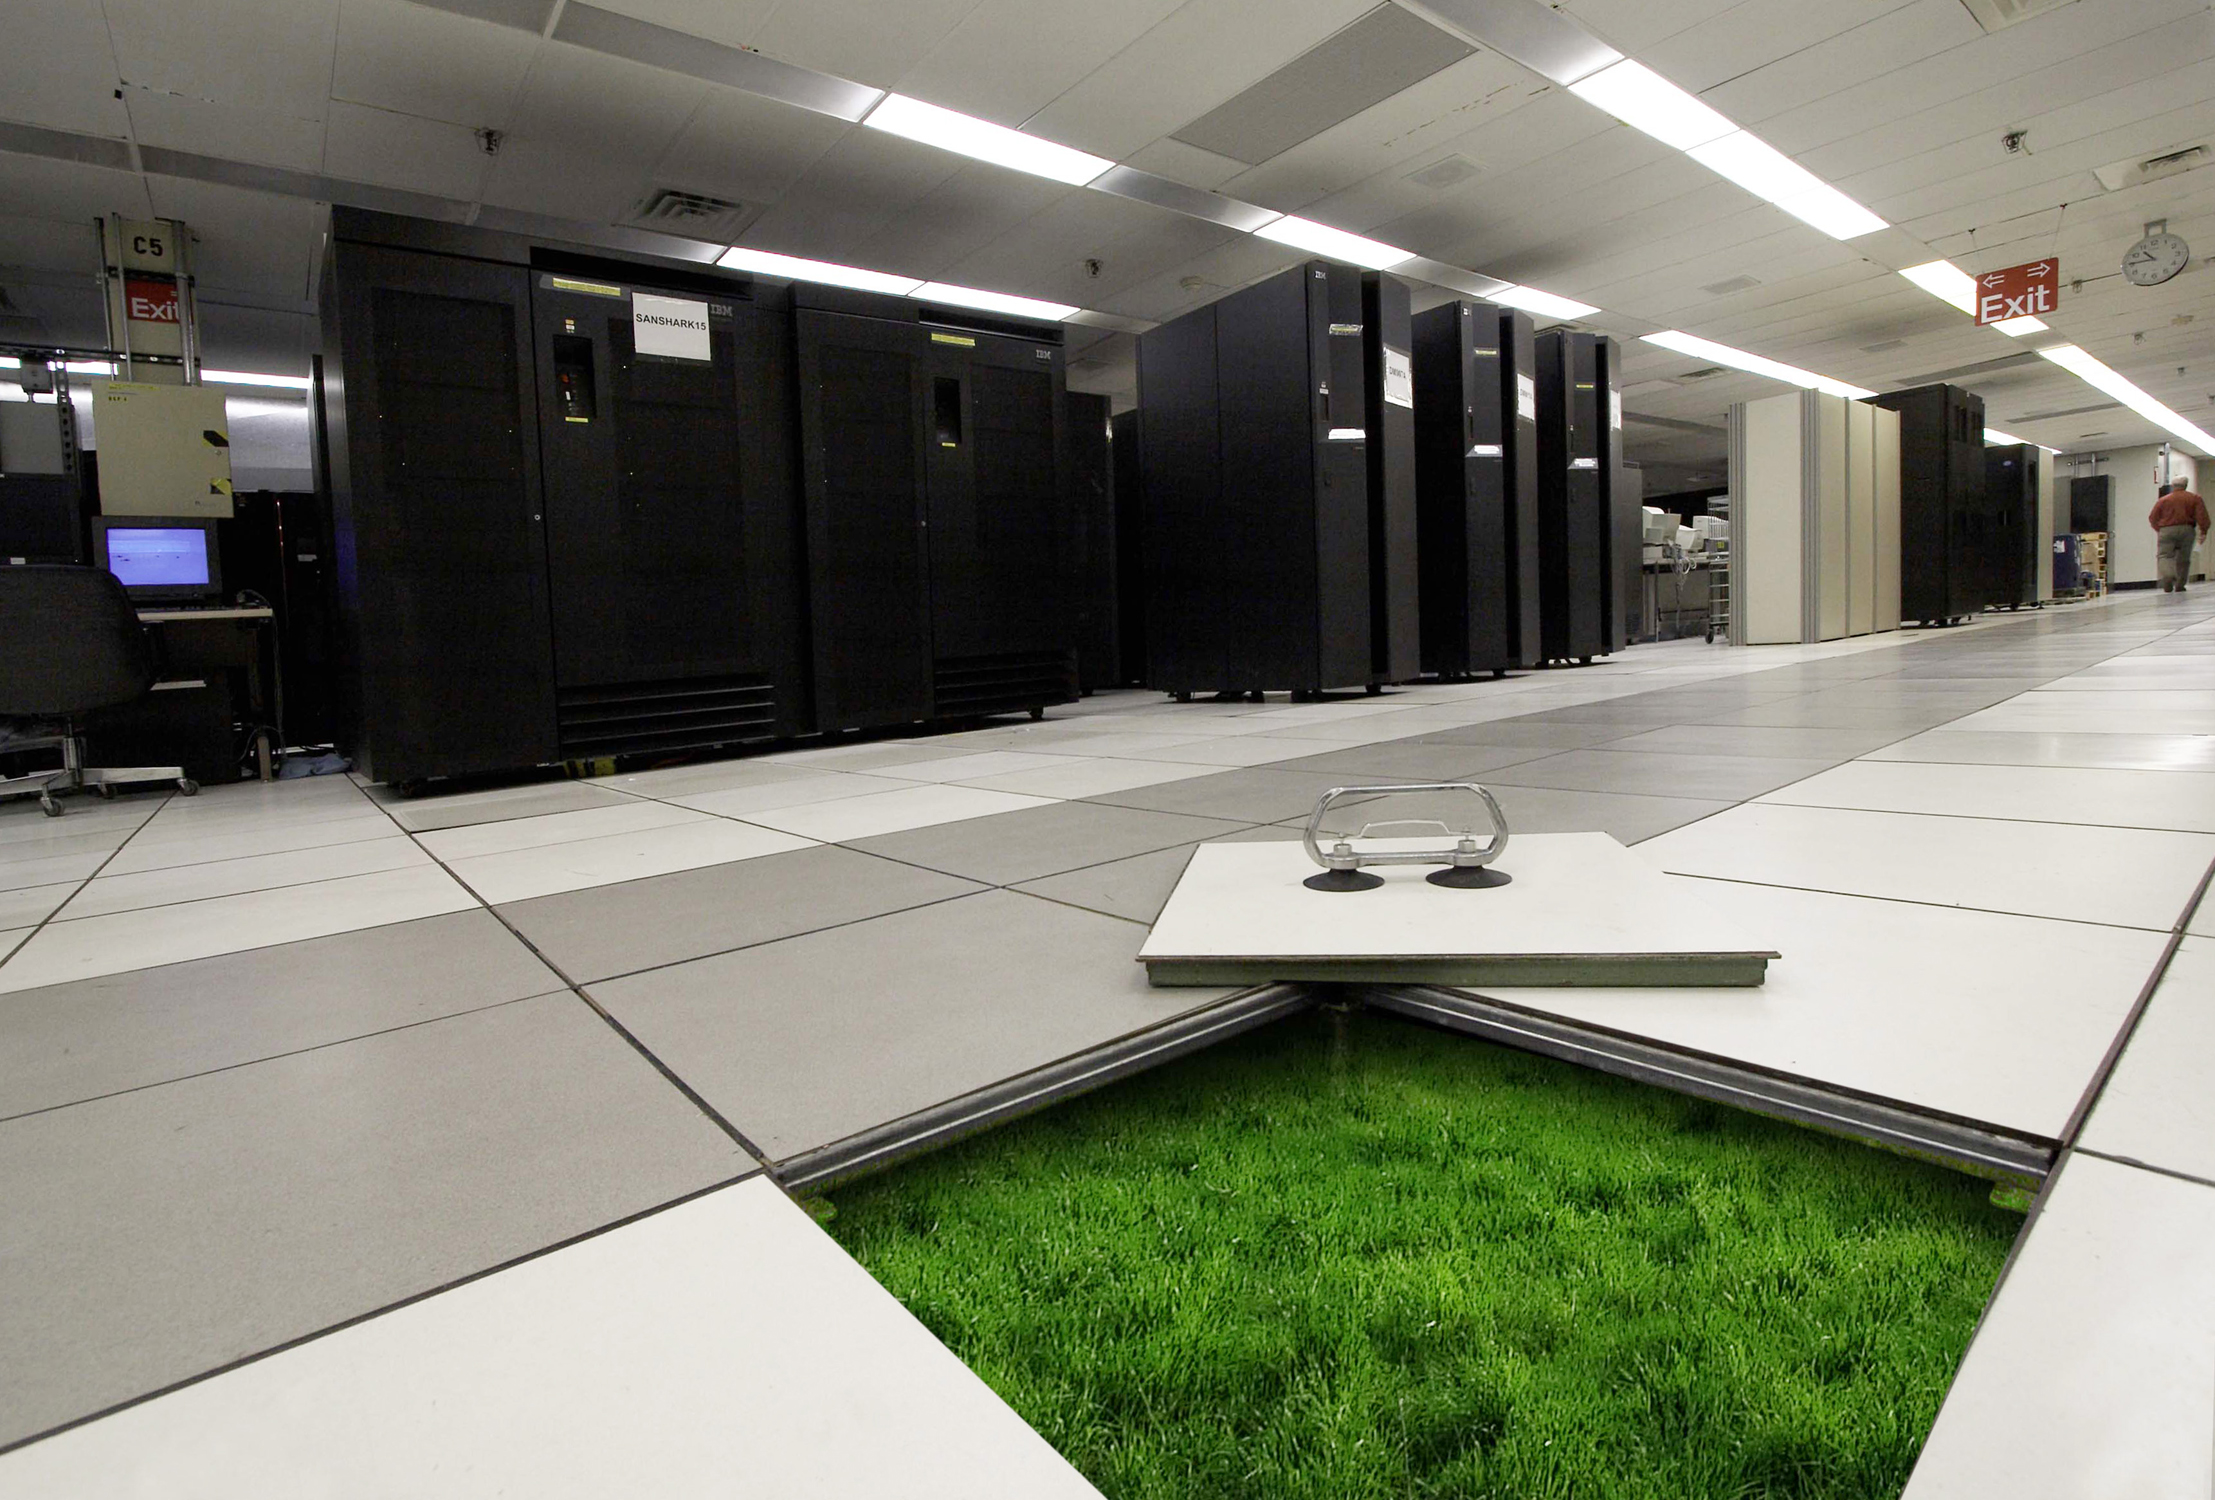
\includegraphics[width=\textwidth]{fig3}
%%	}
%%	\caption{Exemplo de figura inserida em uma página A3 no formato horizontal}
%%	\label{fig5}
%%\end{figure}

%Retornar ao formato A4
%%\clearpage
%%\KOMAoptions{paper=a4, paper=portrait, DIV=15}
%%\recalctypearea
%-- reinicio em A4 


%%\subsubsection{Resumo gráfico}

%%Você pode optar por fazer um resumo no formato de mapa mental/conceitual. 
%%Aqui foi utilizado o site https://app.mindmup.com para gerar o mapa.

%%Para utilizar o resumo gráfico, remova o texto da seção resumo (linha 137) e inclua o código para inserir a figura, conforme figura \ref{fig6}

%%\begin{figure}[h]
%%	\centering
%%	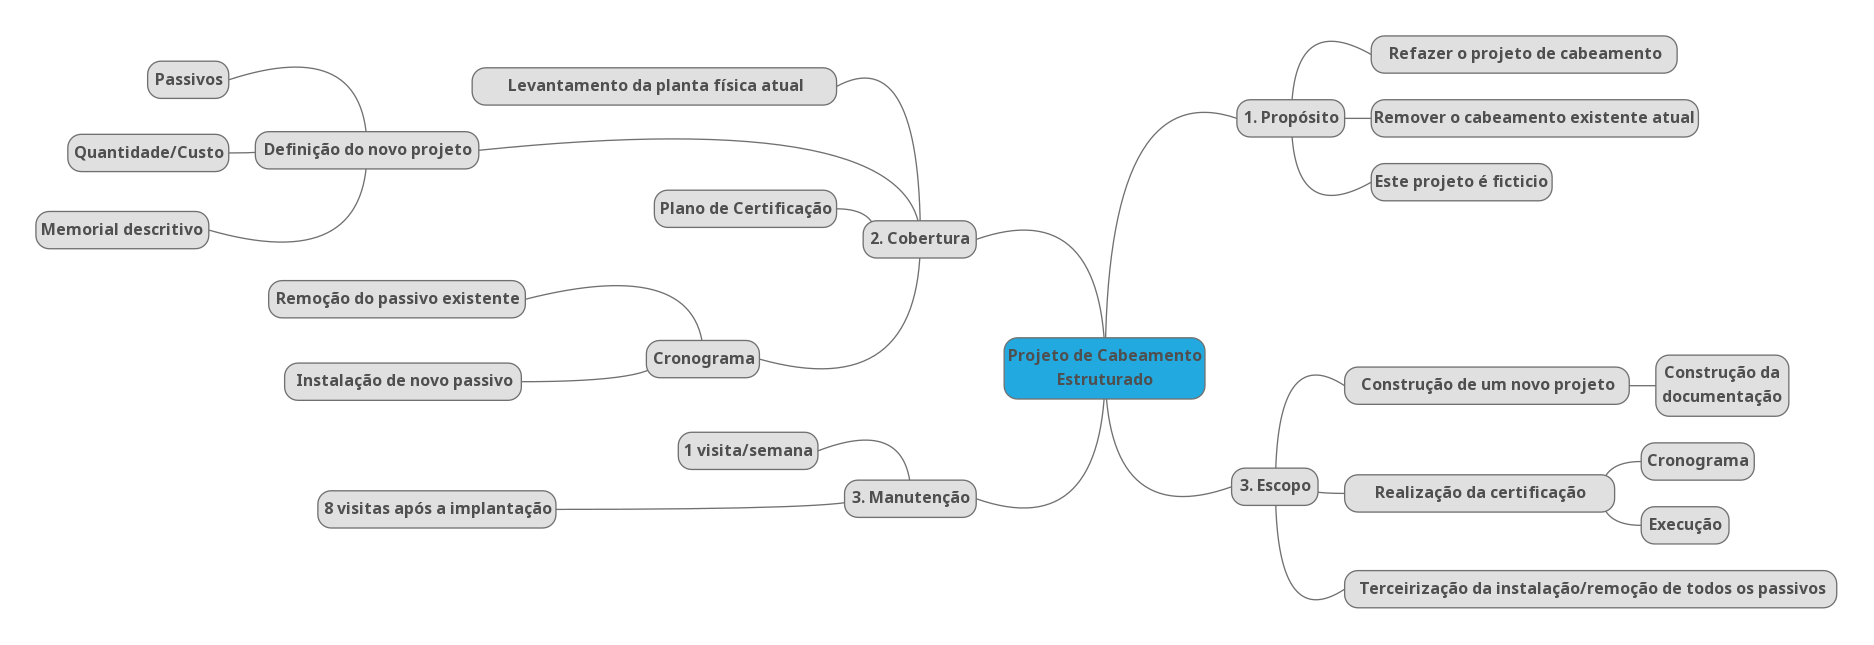
\includegraphics[width=\textwidth,height=5cm,keepaspectratio]{fig4}
%%	\caption{Exemplo de resumo gráfico}
%%	\label{fig6}	
%%\end{figure}

%%\subsubsection{Inserir PDF}

%%Para inserir um arquivo pdf em seu texto utilize o comando includepdf. O arquivo será mapeado no layout corrente.

%%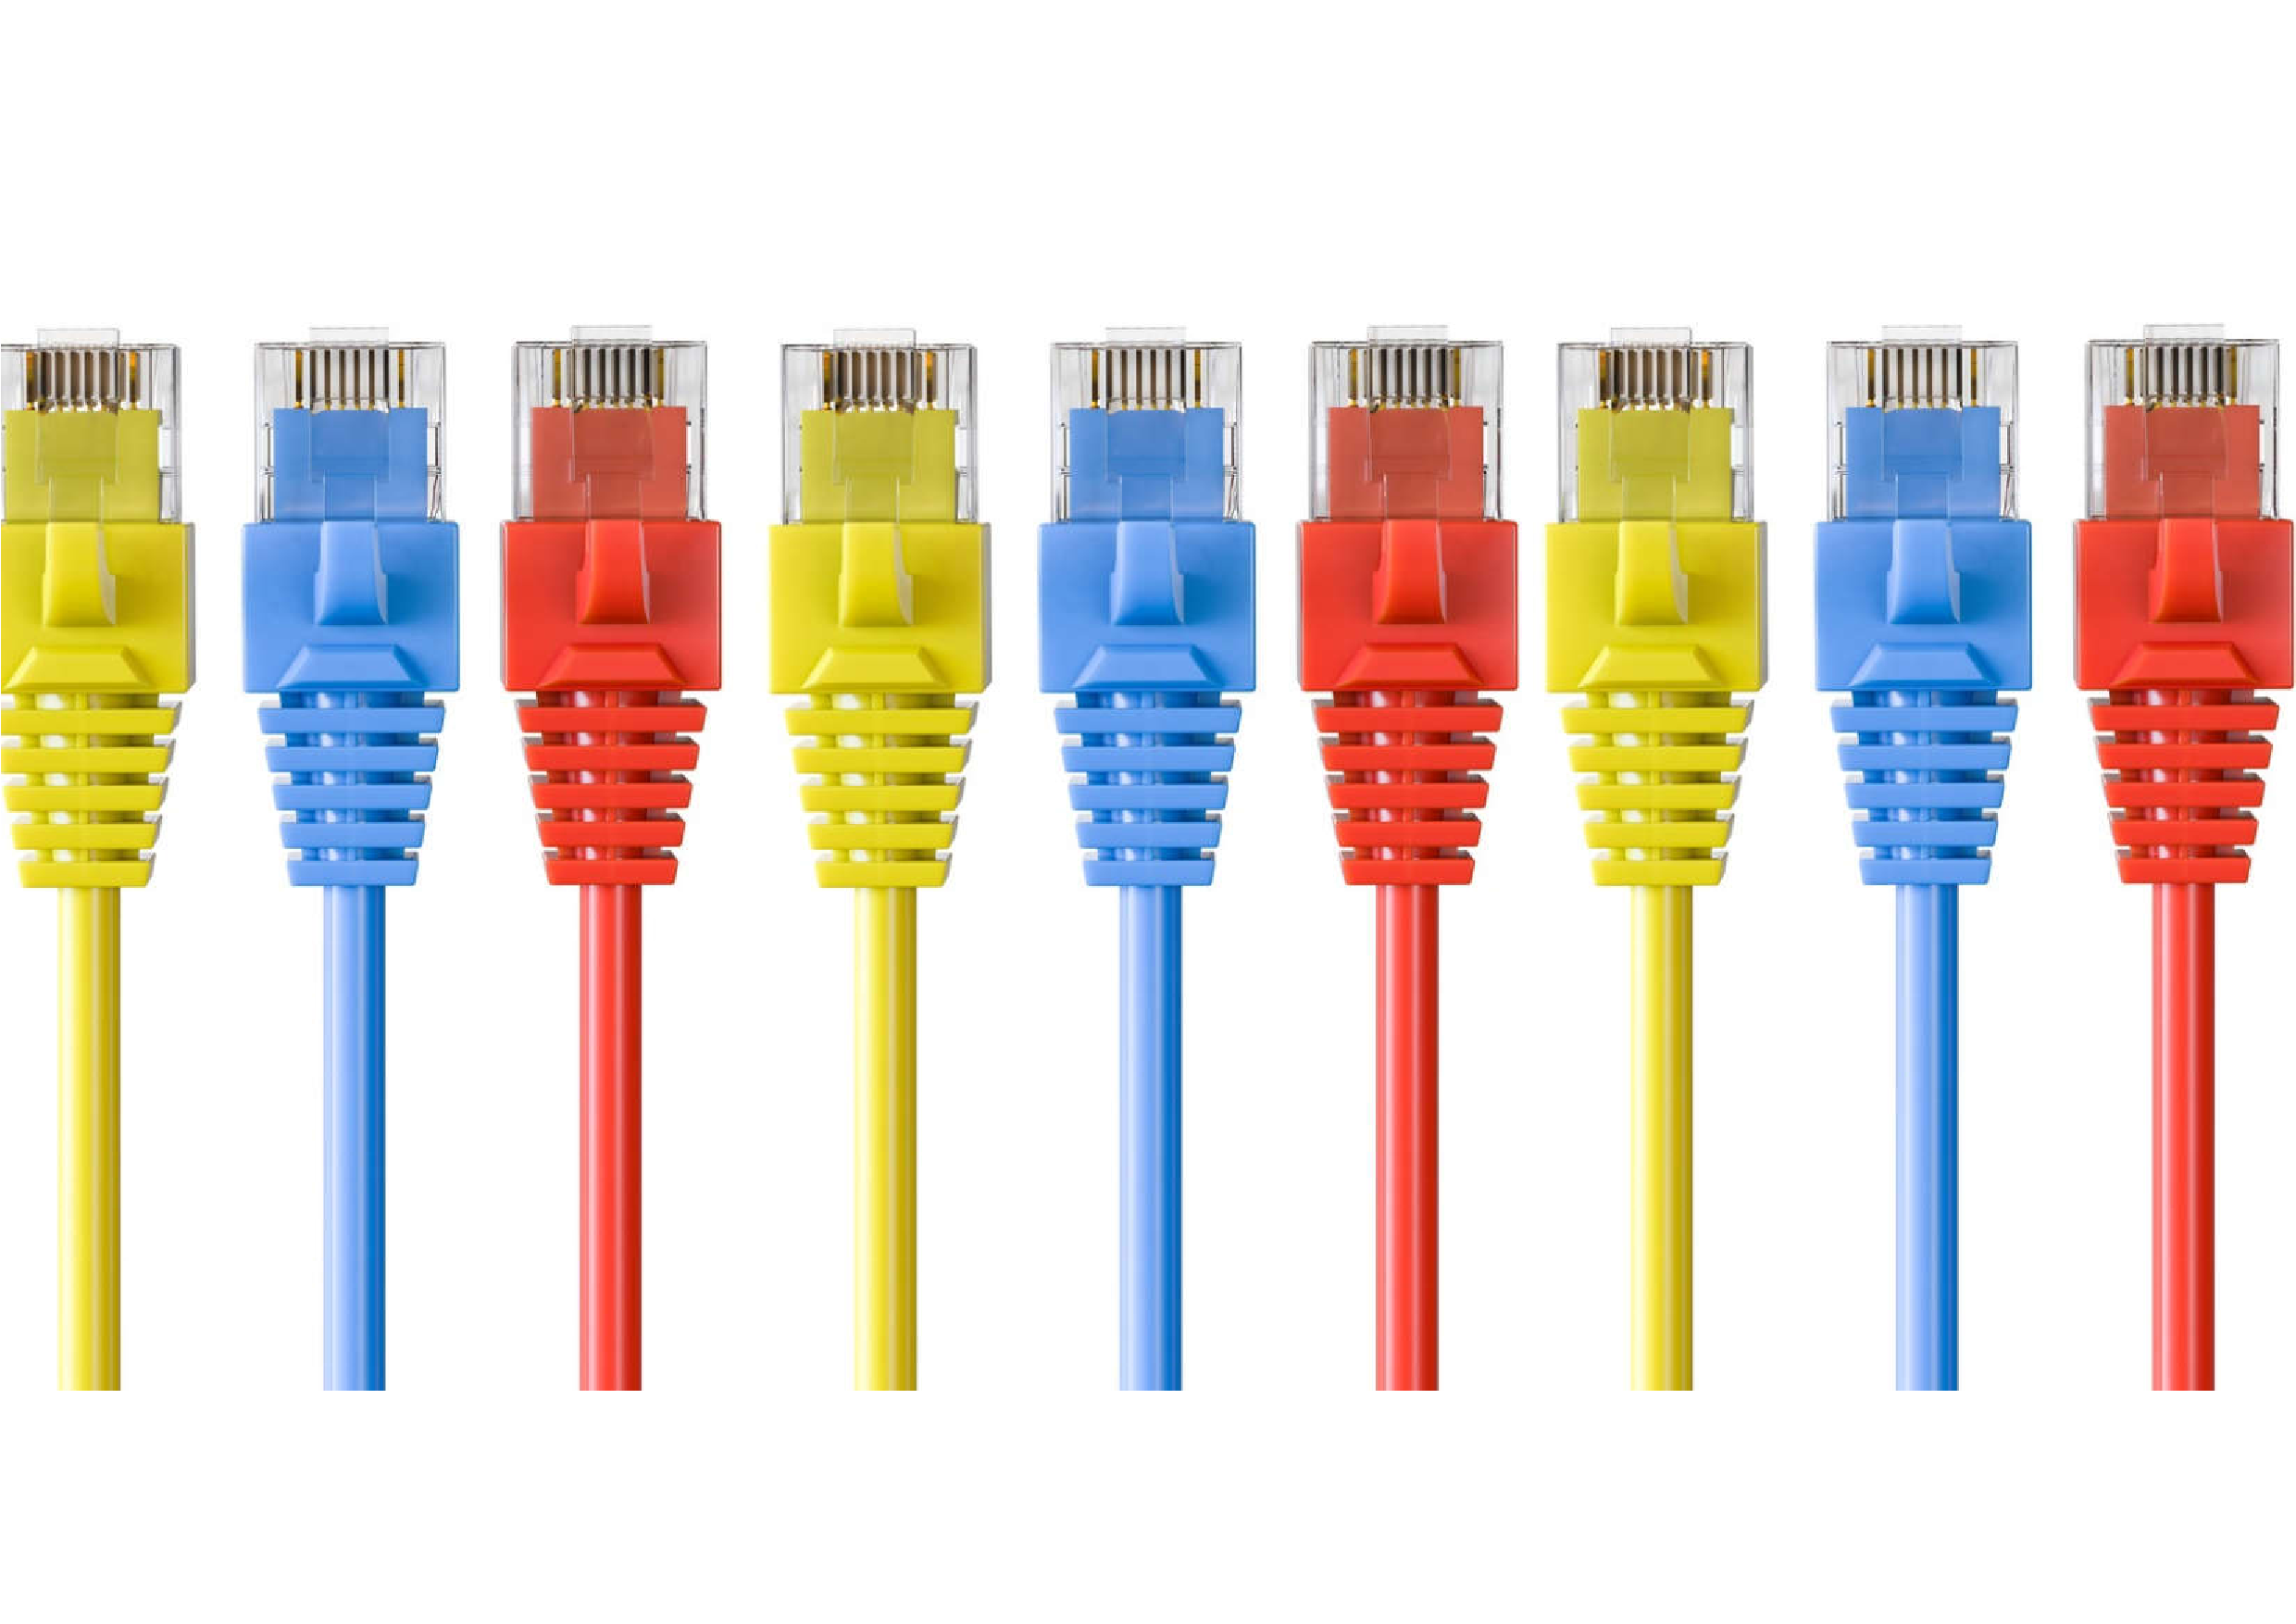
\includepdf{cabling.pdf}
%% ***********************************************************************
%% === ate aqui    =====  ================================================
%% ***********************************************************************

\end{document}